%%%%%%%% ICML 2024 EXAMPLE LATEX SUBMISSION FILE %%%%%%%%%%%%%%%%%

\documentclass{article}

% Recommended, but optional, packages for figures and better typesetting:
\usepackage{microtype}
\usepackage{graphicx}
\usepackage{booktabs} % for professional tables
\usepackage{pgfplots}
\usepackage{pgfplotstable}
\usepackage{hyperref}
\usepackage{tabularray}


% hyperref makes hyperlinks in the resulting PDF.
% If your build breaks (sometimes temporarily if a hyperlink spans a page)
% please comment out the following usepackage line and replace
% \usepackage{icml2024} with \usepackage[nohyperref]{icml2024} above.
\usepackage{hyperref}


% Attempt to make hyperref and algorithmic work together better:
\newcommand{\theHalgorithm}{\arabic{algorithm}}

% Use the following line for the initial blind version submitted for review:
% \usepackage{icml2024}

% If accepted, instead use the following line for the camera-ready submission:
\usepackage[accepted]{icml2024}

% For theorems and such
\usepackage{amsmath}
\usepackage{amssymb}
\usepackage{mathtools}
\usepackage{amsthm}
\usepackage{xspace}
\usepackage{multirow}
\usepackage{tcolorbox}
\usepackage{adjustbox}
\usepackage{makecell}
\usepackage{subfig}
% if you use cleveref..
\usepackage[capitalize,noabbrev]{cleveref}

\usepackage{balance}

\captionsetup[subfloat]{labelformat=simple, labelsep=colon}
\renewcommand{\thesubfigure}{\thefigure.\arabic{subfigure}}

%%%%%%%%%%%%%%%%%%%%%%%%%%%%%%%%
% THEOREMS
%%%%%%%%%%%%%%%%%%%%%%%%%%%%%%%%
\theoremstyle{plain}
\newtheorem{theorem}{Theorem}[section]
\newtheorem{proposition}[theorem]{Proposition}
\newtheorem{lemma}[theorem]{Lemma}
\newtheorem{corollary}[theorem]{Corollary}
\theoremstyle{definition}
\newtheorem{definition}[theorem]{Definition}
\newtheorem{assumption}[theorem]{Assumption}
\theoremstyle{remark}
\newtheorem{remark}[theorem]{Remark}
\pgfplotsset{compat=1.17}

% Todonotes is useful during development; simply uncomment the next line
%    and comment out the line below the next line to turn off comments
%\usepackage[disable,textsize=tiny]{todonotes}
\usepackage[textsize=tiny]{todonotes}
% The \icmltitle you define below is probably too long as a header.
% Therefore, a short form for the running title is supplied here:

\newcommand{\q}[1]{``{#1}''}
\newcommand{\tool}{Deep-Bench\xspace}
\newcommand*\circled[1]{\tikz[baseline=(char.base)]{
            \node[shape=circle,draw,inner sep=2pt] (char) {#1};}}

\icmltitlerunning{\tool: Deep Learning Benchmark Dataset for Code Generation}

\begin{document}


%
\setlength\unitlength{1mm}
\newcommand{\twodots}{\mathinner {\ldotp \ldotp}}
% bb font symbols
\newcommand{\Rho}{\mathrm{P}}
\newcommand{\Tau}{\mathrm{T}}

\newfont{\bbb}{msbm10 scaled 700}
\newcommand{\CCC}{\mbox{\bbb C}}

\newfont{\bb}{msbm10 scaled 1100}
\newcommand{\CC}{\mbox{\bb C}}
\newcommand{\PP}{\mbox{\bb P}}
\newcommand{\RR}{\mbox{\bb R}}
\newcommand{\QQ}{\mbox{\bb Q}}
\newcommand{\ZZ}{\mbox{\bb Z}}
\newcommand{\FF}{\mbox{\bb F}}
\newcommand{\GG}{\mbox{\bb G}}
\newcommand{\EE}{\mbox{\bb E}}
\newcommand{\NN}{\mbox{\bb N}}
\newcommand{\KK}{\mbox{\bb K}}
\newcommand{\HH}{\mbox{\bb H}}
\newcommand{\SSS}{\mbox{\bb S}}
\newcommand{\UU}{\mbox{\bb U}}
\newcommand{\VV}{\mbox{\bb V}}


\newcommand{\yy}{\mathbbm{y}}
\newcommand{\xx}{\mathbbm{x}}
\newcommand{\zz}{\mathbbm{z}}
\newcommand{\sss}{\mathbbm{s}}
\newcommand{\rr}{\mathbbm{r}}
\newcommand{\pp}{\mathbbm{p}}
\newcommand{\qq}{\mathbbm{q}}
\newcommand{\ww}{\mathbbm{w}}
\newcommand{\hh}{\mathbbm{h}}
\newcommand{\vvv}{\mathbbm{v}}

% Vectors

\newcommand{\av}{{\bf a}}
\newcommand{\bv}{{\bf b}}
\newcommand{\cv}{{\bf c}}
\newcommand{\dv}{{\bf d}}
\newcommand{\ev}{{\bf e}}
\newcommand{\fv}{{\bf f}}
\newcommand{\gv}{{\bf g}}
\newcommand{\hv}{{\bf h}}
\newcommand{\iv}{{\bf i}}
\newcommand{\jv}{{\bf j}}
\newcommand{\kv}{{\bf k}}
\newcommand{\lv}{{\bf l}}
\newcommand{\mv}{{\bf m}}
\newcommand{\nv}{{\bf n}}
\newcommand{\ov}{{\bf o}}
\newcommand{\pv}{{\bf p}}
\newcommand{\qv}{{\bf q}}
\newcommand{\rv}{{\bf r}}
\newcommand{\sv}{{\bf s}}
\newcommand{\tv}{{\bf t}}
\newcommand{\uv}{{\bf u}}
\newcommand{\wv}{{\bf w}}
\newcommand{\vv}{{\bf v}}
\newcommand{\xv}{{\bf x}}
\newcommand{\yv}{{\bf y}}
\newcommand{\zv}{{\bf z}}
\newcommand{\zerov}{{\bf 0}}
\newcommand{\onev}{{\bf 1}}

% Matrices

\newcommand{\Am}{{\bf A}}
\newcommand{\Bm}{{\bf B}}
\newcommand{\Cm}{{\bf C}}
\newcommand{\Dm}{{\bf D}}
\newcommand{\Em}{{\bf E}}
\newcommand{\Fm}{{\bf F}}
\newcommand{\Gm}{{\bf G}}
\newcommand{\Hm}{{\bf H}}
\newcommand{\Id}{{\bf I}}
\newcommand{\Jm}{{\bf J}}
\newcommand{\Km}{{\bf K}}
\newcommand{\Lm}{{\bf L}}
\newcommand{\Mm}{{\bf M}}
\newcommand{\Nm}{{\bf N}}
\newcommand{\Om}{{\bf O}}
\newcommand{\Pm}{{\bf P}}
\newcommand{\Qm}{{\bf Q}}
\newcommand{\Rm}{{\bf R}}
\newcommand{\Sm}{{\bf S}}
\newcommand{\Tm}{{\bf T}}
\newcommand{\Um}{{\bf U}}
\newcommand{\Wm}{{\bf W}}
\newcommand{\Vm}{{\bf V}}
\newcommand{\Xm}{{\bf X}}
\newcommand{\Ym}{{\bf Y}}
\newcommand{\Zm}{{\bf Z}}

% Calligraphic

\newcommand{\Ac}{{\cal A}}
\newcommand{\Bc}{{\cal B}}
\newcommand{\Cc}{{\cal C}}
\newcommand{\Dc}{{\cal D}}
\newcommand{\Ec}{{\cal E}}
\newcommand{\Fc}{{\cal F}}
\newcommand{\Gc}{{\cal G}}
\newcommand{\Hc}{{\cal H}}
\newcommand{\Ic}{{\cal I}}
\newcommand{\Jc}{{\cal J}}
\newcommand{\Kc}{{\cal K}}
\newcommand{\Lc}{{\cal L}}
\newcommand{\Mc}{{\cal M}}
\newcommand{\Nc}{{\cal N}}
\newcommand{\nc}{{\cal n}}
\newcommand{\Oc}{{\cal O}}
\newcommand{\Pc}{{\cal P}}
\newcommand{\Qc}{{\cal Q}}
\newcommand{\Rc}{{\cal R}}
\newcommand{\Sc}{{\cal S}}
\newcommand{\Tc}{{\cal T}}
\newcommand{\Uc}{{\cal U}}
\newcommand{\Wc}{{\cal W}}
\newcommand{\Vc}{{\cal V}}
\newcommand{\Xc}{{\cal X}}
\newcommand{\Yc}{{\cal Y}}
\newcommand{\Zc}{{\cal Z}}

% Bold greek letters

\newcommand{\alphav}{\hbox{\boldmath$\alpha$}}
\newcommand{\betav}{\hbox{\boldmath$\beta$}}
\newcommand{\gammav}{\hbox{\boldmath$\gamma$}}
\newcommand{\deltav}{\hbox{\boldmath$\delta$}}
\newcommand{\etav}{\hbox{\boldmath$\eta$}}
\newcommand{\lambdav}{\hbox{\boldmath$\lambda$}}
\newcommand{\epsilonv}{\hbox{\boldmath$\epsilon$}}
\newcommand{\nuv}{\hbox{\boldmath$\nu$}}
\newcommand{\muv}{\hbox{\boldmath$\mu$}}
\newcommand{\zetav}{\hbox{\boldmath$\zeta$}}
\newcommand{\phiv}{\hbox{\boldmath$\phi$}}
\newcommand{\psiv}{\hbox{\boldmath$\psi$}}
\newcommand{\thetav}{\hbox{\boldmath$\theta$}}
\newcommand{\tauv}{\hbox{\boldmath$\tau$}}
\newcommand{\omegav}{\hbox{\boldmath$\omega$}}
\newcommand{\xiv}{\hbox{\boldmath$\xi$}}
\newcommand{\sigmav}{\hbox{\boldmath$\sigma$}}
\newcommand{\piv}{\hbox{\boldmath$\pi$}}
\newcommand{\rhov}{\hbox{\boldmath$\rho$}}
\newcommand{\upsilonv}{\hbox{\boldmath$\upsilon$}}

\newcommand{\Gammam}{\hbox{\boldmath$\Gamma$}}
\newcommand{\Lambdam}{\hbox{\boldmath$\Lambda$}}
\newcommand{\Deltam}{\hbox{\boldmath$\Delta$}}
\newcommand{\Sigmam}{\hbox{\boldmath$\Sigma$}}
\newcommand{\Phim}{\hbox{\boldmath$\Phi$}}
\newcommand{\Pim}{\hbox{\boldmath$\Pi$}}
\newcommand{\Psim}{\hbox{\boldmath$\Psi$}}
\newcommand{\Thetam}{\hbox{\boldmath$\Theta$}}
\newcommand{\Omegam}{\hbox{\boldmath$\Omega$}}
\newcommand{\Xim}{\hbox{\boldmath$\Xi$}}


% Sans Serif small case

\newcommand{\Gsf}{{\sf G}}

\newcommand{\asf}{{\sf a}}
\newcommand{\bsf}{{\sf b}}
\newcommand{\csf}{{\sf c}}
\newcommand{\dsf}{{\sf d}}
\newcommand{\esf}{{\sf e}}
\newcommand{\fsf}{{\sf f}}
\newcommand{\gsf}{{\sf g}}
\newcommand{\hsf}{{\sf h}}
\newcommand{\isf}{{\sf i}}
\newcommand{\jsf}{{\sf j}}
\newcommand{\ksf}{{\sf k}}
\newcommand{\lsf}{{\sf l}}
\newcommand{\msf}{{\sf m}}
\newcommand{\nsf}{{\sf n}}
\newcommand{\osf}{{\sf o}}
\newcommand{\psf}{{\sf p}}
\newcommand{\qsf}{{\sf q}}
\newcommand{\rsf}{{\sf r}}
\newcommand{\ssf}{{\sf s}}
\newcommand{\tsf}{{\sf t}}
\newcommand{\usf}{{\sf u}}
\newcommand{\wsf}{{\sf w}}
\newcommand{\vsf}{{\sf v}}
\newcommand{\xsf}{{\sf x}}
\newcommand{\ysf}{{\sf y}}
\newcommand{\zsf}{{\sf z}}


% mixed symbols

\newcommand{\sinc}{{\hbox{sinc}}}
\newcommand{\diag}{{\hbox{diag}}}
\renewcommand{\det}{{\hbox{det}}}
\newcommand{\trace}{{\hbox{tr}}}
\newcommand{\sign}{{\hbox{sign}}}
\renewcommand{\arg}{{\hbox{arg}}}
\newcommand{\var}{{\hbox{var}}}
\newcommand{\cov}{{\hbox{cov}}}
\newcommand{\Ei}{{\rm E}_{\rm i}}
\renewcommand{\Re}{{\rm Re}}
\renewcommand{\Im}{{\rm Im}}
\newcommand{\eqdef}{\stackrel{\Delta}{=}}
\newcommand{\defines}{{\,\,\stackrel{\scriptscriptstyle \bigtriangleup}{=}\,\,}}
\newcommand{\<}{\left\langle}
\renewcommand{\>}{\right\rangle}
\newcommand{\herm}{{\sf H}}
\newcommand{\trasp}{{\sf T}}
\newcommand{\transp}{{\sf T}}
\renewcommand{\vec}{{\rm vec}}
\newcommand{\Psf}{{\sf P}}
\newcommand{\SINR}{{\sf SINR}}
\newcommand{\SNR}{{\sf SNR}}
\newcommand{\MMSE}{{\sf MMSE}}
\newcommand{\REF}{{\RED [REF]}}

% Markov chain
\usepackage{stmaryrd} % for \mkv 
\newcommand{\mkv}{-\!\!\!\!\minuso\!\!\!\!-}

% Colors

\newcommand{\RED}{\color[rgb]{1.00,0.10,0.10}}
\newcommand{\BLUE}{\color[rgb]{0,0,0.90}}
\newcommand{\GREEN}{\color[rgb]{0,0.80,0.20}}

%%%%%%%%%%%%%%%%%%%%%%%%%%%%%%%%%%%%%%%%%%
\usepackage{hyperref}
\hypersetup{
    bookmarks=true,         % show bookmarks bar?
    unicode=false,          % non-Latin characters in AcrobatÕs bookmarks
    pdftoolbar=true,        % show AcrobatÕs toolbar?
    pdfmenubar=true,        % show AcrobatÕs menu?
    pdffitwindow=false,     % window fit to page when opened
    pdfstartview={FitH},    % fits the width of the page to the window
%    pdftitle={My title},    % title
%    pdfauthor={Author},     % author
%    pdfsubject={Subject},   % subject of the document
%    pdfcreator={Creator},   % creator of the document
%    pdfproducer={Producer}, % producer of the document
%    pdfkeywords={keyword1} {key2} {key3}, % list of keywords
    pdfnewwindow=true,      % links in new window
    colorlinks=true,       % false: boxed links; true: colored links
    linkcolor=red,          % color of internal links (change box color with linkbordercolor)
    citecolor=green,        % color of links to bibliography
    filecolor=blue,      % color of file links
    urlcolor=blue           % color of external links
}
%%%%%%%%%%%%%%%%%%%%%%%%%%%%%%%%%%%%%%%%%%%



\twocolumn[
    \icmltitle{\tool: Deep Learning Benchmark Dataset for Code Generation}

    % You may provide any keywords that you
    % find helpful for describing your paper; these are used to populate
    % the "keywords" metadata in the PDF but will not be shown in the document
    % It is OKAY to include author information, even for blind
% submissions: the style file will automatically remove it for you
% unless you've provided the [accepted] option to the icml2024
% package.

% List of affiliations: The first argument should be a (short)
% identifier you will use later to specify author affiliations
% Academic affiliations should list Department, University, City, Region, Country
% Industry affiliations should list Company, City, Region, Country

% You can specify symbols, otherwise they are numbered in order.
% Ideally, you should not use this facility. Affiliations will be numbered
% in order of appearance and this is the preferred way.
\icmlsetsymbol{equal}{*}

\begin{icmlauthorlist}
\icmlauthor{Alireza Daghighfarsoodeh}{yyy}
\icmlauthor{Chung-Yu Wang}{yyy}
\icmlauthor{Hamed Taherkhani}{yyy}
\icmlauthor{Melika Sepidband}{yyy}
\icmlauthor{Mohammad Abdollahi}{yyy}
\icmlauthor{Hadi Hemmati}{yyy}
\icmlauthor{Hung Viet Pham}{yyy}
%\icmlauthor{}{sch}
%\icmlauthor{}{sch}
%\icmlauthor{}{sch}
\end{icmlauthorlist}

\icmlaffiliation{yyy}{Department of EECS, York University, Toronto, Canada}

    \icmlkeywords{Benchmark, Large Language Model, ICML}
    
\vskip 0.3in
]



\begin{abstract}
\begin{abstract}


The choice of representation for geographic location significantly impacts the accuracy of models for a broad range of geospatial tasks, including fine-grained species classification, population density estimation, and biome classification. Recent works like SatCLIP and GeoCLIP learn such representations by contrastively aligning geolocation with co-located images. While these methods work exceptionally well, in this paper, we posit that the current training strategies fail to fully capture the important visual features. We provide an information theoretic perspective on why the resulting embeddings from these methods discard crucial visual information that is important for many downstream tasks. To solve this problem, we propose a novel retrieval-augmented strategy called RANGE. We build our method on the intuition that the visual features of a location can be estimated by combining the visual features from multiple similar-looking locations. We evaluate our method across a wide variety of tasks. Our results show that RANGE outperforms the existing state-of-the-art models with significant margins in most tasks. We show gains of up to 13.1\% on classification tasks and 0.145 $R^2$ on regression tasks. All our code and models will be made available at: \href{https://github.com/mvrl/RANGE}{https://github.com/mvrl/RANGE}.

\end{abstract}


\end{abstract}

\section{Introduction}
Backdoor attacks pose a concealed yet profound security risk to machine learning (ML) models, for which the adversaries can inject a stealth backdoor into the model during training, enabling them to illicitly control the model's output upon encountering predefined inputs. These attacks can even occur without the knowledge of developers or end-users, thereby undermining the trust in ML systems. As ML becomes more deeply embedded in critical sectors like finance, healthcare, and autonomous driving \citep{he2016deep, liu2020computing, tournier2019mrtrix3, adjabi2020past}, the potential damage from backdoor attacks grows, underscoring the emergency for developing robust defense mechanisms against backdoor attacks.

To address the threat of backdoor attacks, researchers have developed a variety of strategies \cite{liu2018fine,wu2021adversarial,wang2019neural,zeng2022adversarial,zhu2023neural,Zhu_2023_ICCV, wei2024shared,wei2024d3}, aimed at purifying backdoors within victim models. These methods are designed to integrate with current deployment workflows seamlessly and have demonstrated significant success in mitigating the effects of backdoor triggers \cite{wubackdoorbench, wu2023defenses, wu2024backdoorbench,dunnett2024countering}.  However, most state-of-the-art (SOTA) backdoor purification methods operate under the assumption that a small clean dataset, often referred to as \textbf{auxiliary dataset}, is available for purification. Such an assumption poses practical challenges, especially in scenarios where data is scarce. To tackle this challenge, efforts have been made to reduce the size of the required auxiliary dataset~\cite{chai2022oneshot,li2023reconstructive, Zhu_2023_ICCV} and even explore dataset-free purification techniques~\cite{zheng2022data,hong2023revisiting,lin2024fusing}. Although these approaches offer some improvements, recent evaluations \cite{dunnett2024countering, wu2024backdoorbench} continue to highlight the importance of sufficient auxiliary data for achieving robust defenses against backdoor attacks.

While significant progress has been made in reducing the size of auxiliary datasets, an equally critical yet underexplored question remains: \emph{how does the nature of the auxiliary dataset affect purification effectiveness?} In  real-world  applications, auxiliary datasets can vary widely, encompassing in-distribution data, synthetic data, or external data from different sources. Understanding how each type of auxiliary dataset influences the purification effectiveness is vital for selecting or constructing the most suitable auxiliary dataset and the corresponding technique. For instance, when multiple datasets are available, understanding how different datasets contribute to purification can guide defenders in selecting or crafting the most appropriate dataset. Conversely, when only limited auxiliary data is accessible, knowing which purification technique works best under those constraints is critical. Therefore, there is an urgent need for a thorough investigation into the impact of auxiliary datasets on purification effectiveness to guide defenders in  enhancing the security of ML systems. 

In this paper, we systematically investigate the critical role of auxiliary datasets in backdoor purification, aiming to bridge the gap between idealized and practical purification scenarios.  Specifically, we first construct a diverse set of auxiliary datasets to emulate real-world conditions, as summarized in Table~\ref{overall}. These datasets include in-distribution data, synthetic data, and external data from other sources. Through an evaluation of SOTA backdoor purification methods across these datasets, we uncover several critical insights: \textbf{1)} In-distribution datasets, particularly those carefully filtered from the original training data of the victim model, effectively preserve the model’s utility for its intended tasks but may fall short in eliminating backdoors. \textbf{2)} Incorporating OOD datasets can help the model forget backdoors but also bring the risk of forgetting critical learned knowledge, significantly degrading its overall performance. Building on these findings, we propose Guided Input Calibration (GIC), a novel technique that enhances backdoor purification by adaptively transforming auxiliary data to better align with the victim model’s learned representations. By leveraging the victim model itself to guide this transformation, GIC optimizes the purification process, striking a balance between preserving model utility and mitigating backdoor threats. Extensive experiments demonstrate that GIC significantly improves the effectiveness of backdoor purification across diverse auxiliary datasets, providing a practical and robust defense solution.

Our main contributions are threefold:
\textbf{1) Impact analysis of auxiliary datasets:} We take the \textbf{first step}  in systematically investigating how different types of auxiliary datasets influence backdoor purification effectiveness. Our findings provide novel insights and serve as a foundation for future research on optimizing dataset selection and construction for enhanced backdoor defense.
%
\textbf{2) Compilation and evaluation of diverse auxiliary datasets:}  We have compiled and rigorously evaluated a diverse set of auxiliary datasets using SOTA purification methods, making our datasets and code publicly available to facilitate and support future research on practical backdoor defense strategies.
%
\textbf{3) Introduction of GIC:} We introduce GIC, the \textbf{first} dedicated solution designed to align auxiliary datasets with the model’s learned representations, significantly enhancing backdoor mitigation across various dataset types. Our approach sets a new benchmark for practical and effective backdoor defense.



\section{Related Work}
\label{sec:related-works}
\subsection{Novel View Synthesis}
Novel view synthesis is a foundational task in the computer vision and graphics, which aims to generate unseen views of a scene from a given set of images.
% Many methods have been designed to solve this problem by posing it as 3D geometry based rendering, where point clouds~\cite{point_differentiable,point_nfs}, mesh~\cite{worldsheet,FVS,SVS}, planes~\cite{automatci_photo_pop_up,tour_into_the_picture} and multi-plane images~\cite{MINE,single_view_mpi,stereo_magnification}, \etal
Numerous methods have been developed to address this problem by approaching it as 3D geometry-based rendering, such as using meshes~\cite{worldsheet,FVS,SVS}, MPI~\cite{MINE,single_view_mpi,stereo_magnification}, point clouds~\cite{point_differentiable,point_nfs}, etc.
% planes~\cite{automatci_photo_pop_up,tour_into_the_picture}, 


\begin{figure*}[!t]
    \centering
    \includegraphics[width=1.0\linewidth]{figures/overview-v7.png}
    %\caption{\textbf{Overview.} Given a set of images, our method obtains both camera intrinsics and extrinsics, as well as a 3DGS model. First, we obtain the initial camera parameters, global track points from image correspondences and monodepth with reprojection loss. Then we incorporate the global track information and select Gaussian kernels associated with track points. We jointly optimize the parameters $K$, $T_{cw}$, 3DGS through multi-view geometric consistency $L_{t2d}$, $L_{t3d}$, $L_{scale}$ and photometric consistency $L_1$, $L_{D-SSIM}$.}
    \caption{\textbf{Overview.} Given a set of images, our method obtains both camera intrinsics and extrinsics, as well as a 3DGS model. During the initialization, we extract the global tracks, and initialize camera parameters and Gaussians from image correspondences and monodepth with reprojection loss. We determine Gaussian kernels with recovered 3D track points, and then jointly optimize the parameters $K$, $T_{cw}$, 3DGS through the proposed global track constraints (i.e., $L_{t2d}$, $L_{t3d}$, and $L_{scale}$) and original photometric losses (i.e., $L_1$ and $L_{D-SSIM}$).}
    \label{fig:overview}
\end{figure*}

Recently, Neural Radiance Fields (NeRF)~\cite{2020NeRF} provide a novel solution to this problem by representing scenes as implicit radiance fields using neural networks, achieving photo-realistic rendering quality. Although having some works in improving efficiency~\cite{instant_nerf2022, lin2022enerf}, the time-consuming training and rendering still limit its practicality.
Alternatively, 3D Gaussian Splatting (3DGS)~\cite{3DGS2023} models the scene as explicit Gaussian kernels, with differentiable splatting for rendering. Its improved real-time rendering performance, lower storage and efficiency, quickly attract more attentions.
% Different from NeRF-based methods which need MLPs to model the scene and huge computational cost for rendering, 3DGS has stronger real-time performance, higher storage and computational efficiency, benefits from its explicit representation and gradient backpropagation.

\subsection{Optimizing Camera Poses in NeRFs and 3DGS}
Although NeRF and 3DGS can provide impressive scene representation, these methods all need accurate camera parameters (both intrinsic and extrinsic) as additional inputs, which are mostly obtained by COLMAP~\cite{colmap2016}.
% This strong reliance on COLMAP significantly limits their use in real-world applications, so optimizing the camera parameters during the scene training becomes crucial.
When the prior is inaccurate or unknown, accurately estimating camera parameters and scene representations becomes crucial.

% In early works, only photometric constraints are used for scene training and camera pose estimation. 
% iNeRF~\cite{iNerf2021} optimizes the camera poses based on a pre-trained NeRF model.
% NeRFmm~\cite{wang2021nerfmm} introduce a joint optimization process, which estimates the camera poses and trains NeRF model jointly.
% BARF~\cite{barf2021} and GARF~\cite{2022GARF} provide new positional encoding strategy to handle with the gradient inconsistency issue of positional embedding and yield promising results.
% However, they achieve satisfactory optimization results when only the pose initialization is quite closed to the ground-truth, as the photometric constrains can only improve the quality of camera estimation within a small range.
% Later, more prior information of geometry and correspondence, \ie monocular depth and feature matching, are introduced into joint optimisation to enhance the capability of camera poses estimation.
% SC-NeRF~\cite{SCNeRF2021} minimizes a projected ray distance loss based on correspondence of adjacent frames.
% NoPe-NeRF~\cite{bian2022nopenerf} chooses monocular depth maps as geometric priors, and defines undistorted depth loss and relative pose constraints for joint optimization.
In earlier studies, scene training and camera pose estimation relied solely on photometric constraints. iNeRF~\cite{iNerf2021} refines the camera poses using a pre-trained NeRF model. NeRFmm~\cite{wang2021nerfmm} introduces a joint optimization approach that simultaneously estimates camera poses and trains the NeRF model. BARF~\cite{barf2021} and GARF~\cite{2022GARF} propose a new positional encoding strategy to address the gradient inconsistency issues in positional embedding, achieving promising results. However, these methods only yield satisfactory optimization when the initial pose is very close to the ground truth, as photometric constraints alone can only enhance camera estimation quality within a limited range. Subsequently, 
% additional prior information on geometry and correspondence, such as monocular depth and feature matching, has been incorporated into joint optimization to improve the accuracy of camera pose estimation. 
SC-NeRF~\cite{SCNeRF2021} minimizes a projected ray distance loss based on correspondence between adjacent frames. NoPe-NeRF~\cite{bian2022nopenerf} utilizes monocular depth maps as geometric priors and defines undistorted depth loss and relative pose constraints.

% With regard to 3D Gaussian Splatting, CF-3DGS~\cite{CF-3DGS-2024} also leverages mono-depth information to constrain the optimization of local 3DGS for relative pose estimation and later learn a global 3DGS progressively in a sequential manner.
% InstantSplat~\cite{fan2024instantsplat} focus on sparse view scenes, first use DUSt3R~\cite{dust3r2024cvpr} to generate a set of densely covered and pixel-aligned points for 3D Gaussian initialization, then introduce a parallel grid partitioning strategy in joint optimization to speed up.
% % Jiang et al.~\cite{Jiang_2024sig} proposed to build the scene continuously and progressively, to next unregistered frame, they use registration and adjustment to adjust the previous registered camera poses and align unregistered monocular depths, later refine the joint model by matching detected correspondences in screen-space coordinates.
% \gjh{Jiang et al.~\cite{Jiang_2024sig} also implemented an incremental approach for reconstructing camera poses and scenes. Initially, they perform feature matching between the current image and the image rendered by a differentiable surface renderer. They then construct matching point errors, depth errors, and photometric errors to achieve the registration and adjustment of the current image. Finally, based on the depth map, the pixels of the current image are projected as new 3D Gaussians. However, this method still exhibits limitations when dealing with complex scenes and unordered images.}
% % CG-3DGS~\cite{sun2024correspondenceguidedsfmfree3dgaussian} follows CF-3DGS, first construct a coarse point cloud from mono-depth maps to train a 3DGS model, then progressively estimate camera poses based on this pre-trained model by constraining the correspondences between rendering view and ground-truth.
% \gjh{Similarly, CG-3DGS~\cite{sun2024correspondenceguidedsfmfree3dgaussian} first utilizes monocular depth estimation and the camera parameters from the first frame to initialize a set of 3D Gaussians. It then progressively estimates camera poses based on this pre-trained model by constraining the correspondences between the rendered views and the ground truth.}
% % Free-SurGS~\cite{freesurgs2024} matches the projection flow derived from 3D Gaussians with optical flow to estimate the poses, to compensate for the limitations of photometric loss.
% \gjh{Free-SurGS~\cite{freesurgs2024} introduces the first SfM-free 3DGS approach for surgical scene reconstruction. Due to the challenges posed by weak textures and photometric inconsistencies in surgical scenes, Free-SurGS achieves pose estimation by minimizing the flow loss between the projection flow and the optical flow. Subsequently, it keeps the camera pose fixed and optimizes the scene representation by minimizing the photometric loss, depth loss and flow loss.}
% \gjh{However, most current works assume camera intrinsics are known and primarily focus on optimizing camera poses. Additionally, these methods typically rely on sequentially ordered image inputs and incrementally optimize camera parameters and scene representation. This inevitably leads to drift errors, preventing the achievement of globally consistent results. Our work aims to address these issues.}

Regarding 3D Gaussian Splatting, CF-3DGS~\cite{CF-3DGS-2024} utilizes mono-depth information to refine the optimization of local 3DGS for relative pose estimation and subsequently learns a global 3DGS in a sequential manner. InstantSplat~\cite{fan2024instantsplat} targets sparse view scenes, initially employing DUSt3R~\cite{dust3r2024cvpr} to create a densely covered, pixel-aligned point set for initializing 3D Gaussian models, and then implements a parallel grid partitioning strategy to accelerate joint optimization. Jiang \etal~\cite{Jiang_2024sig} develops an incremental method for reconstructing camera poses and scenes, but it struggles with complex scenes and unordered images. 
% Similarly, CG-3DGS~\cite{sun2024correspondenceguidedsfmfree3dgaussian} progressively estimates camera poses using a pre-trained model by aligning the correspondences between rendered views and actual scenes. Free-SurGS~\cite{freesurgs2024} pioneers an SfM-free 3DGS method for reconstructing surgical scenes, overcoming challenges such as weak textures and photometric inconsistencies by minimizing the discrepancy between projection flow and optical flow.
%\pb{SF-3DGS-HT~\cite{ji2024sfmfree3dgaussiansplatting} introduced VFI into training as additional photometric constraints. They separated the whole scene into several local 3DGS models and then merged them hierarchically, which leads to a significant improvement on simple and dense view scenes.}
HT-3DGS~\cite{ji2024sfmfree3dgaussiansplatting} interpolates frames for training and splits the scene into local clips, using a hierarchical strategy to build 3DGS model. It works well for simple scenes, but fails with dramatic motions due to unstable interpolation and low efficiency.
% {While effective for simple scenes, it struggles with dramatic motion due to unstable view interpolation and suffers from low computational efficiency.}

However, most existing methods generally depend on sequentially ordered image inputs and incrementally optimize camera parameters and 3DGS, which often leads to drift errors and hinders achieving globally consistent results. Our work seeks to overcome these limitations.

\section{Benchmark Construction}
\label{sec:BenchConstr}

\begin{figure*}[t]
    \centering
    \includegraphics[width=0.90\linewidth]{figures/pipeline.pdf}
    \vspace{-2mm}
    \caption{Overall pipeline of proposed {\ours}. An encoded low-resolution video latent is concatenated to the current noisy latent $x_t$, and it undergoes alternating denoising processes using both {\ssi} (\ssiabb) and {\tfi} (\tfiabb). At this stage, the noisy latent is split and merged before and after the denoising process, respectively. 
    After each denoising step, {\drg} ({\drgabb}) is applied to enhance the quality of the image further.}
    \vspace{-2mm}
    \Description{pipeline}
    \label{fig:main}
\end{figure*}
\begin{figure}
    \centering
    \includegraphics[width=\linewidth]{figs/last_template.pdf}
    %\vspace{-7pt}
    \caption{Template of generating prompt from code}
    
    \label{fig:code_prompt}
    \vspace{-10pt}
    
\end{figure}
%\subsection{Overview}

\tool consists of 520 instances of AI and DL data points (filtered from over 2,000 raw data points). The data is curated from 30 GitHub repositories (selected from an initial pool of 160 related repositories).

%In this section, we will discuss the step-by-step process of constructing \tool as demonstrated in Figure~\ref{fig:pipeline}. 
The construction process of \tool consists of two main phases: The Raw Data Extraction and the Labeling Procedure. The raw data extraction involves six semi-automatic steps. Since \tool is designed to have diverse and realistic code samples, the first step \circled{1} is to construct \tool from code crawled from highly rated GitHub repositories (i.e., with the most stars) filtered using 30 DL-related terms such as ``neural-networks'',  ``pytorch'', ``computer-vision''. We then manually select (step \circled{2}) 160 high quality candidate DL projects 
%that are considered DL related 
%to make DL benchmark in code generation, as they 
(i.e., involve the integration of DL and AI-related frameworks, comprehensive test cases, clear and well-written docstrings, and detailed contribution guidelines). We then employed a bespoke utility to extract the test files and then test cases from each repository (step \circled{3} and \circled{4}). By performing static analysis, we were able to track and collect all of the functions under test in step \circled{5} to form the raw data that is the base of \tool. 

Once the raw data is extracted, the labeling procedure starts. To speed up the task of constructing the prompt for each code sample, we utilize LLM (i.e., GPT-4o) as a code-explanation tool\cite{nam2024using} to generate the first prompt candidate for each function under test (step \circled{7}). Four co-authors were then tasked with manually filtering each entry to ensure that each function is highly relevant (i.e., contributes to a DL task such as image recognition, utilizes at least one recognized DL framework, and implements a relatively advanced and sophisticated algorithm).
Finally, we conduct a manual labeling process involving four co-authors (step \circled{9}) to refine the prompt and label each code sample with the appropriate category from our three chosen types of categories: DL pipeline phases, ML task types, and input types.


% (melika) It's better to explain how you generate the prompts. You just mentioned that they are generated automatically.
%In summary, the steps needed for building \tool is as follows:
%\begin{enumerate}
%    \item We gathered 30 different GitHub tags related to deep learning, like ``neural-networks'' (details in Section~\ref{sec:rs}).
%    \item We crawled GitHub and extracted related repositories with those tags, filtering for those that were more recently updated and had more than 400 stars (details in Section~\ref{sec:rs}).
%    \item We manually cherry-picked 160 repositories for more detailed data extraction and cloned them (details in Section~\ref{sec:rs}).
%    \item We extracted test cases within each repository (details in Section~\ref{sec:fe}).
%    \item We then extracted functions that are called in the test suites, ensuring they were not third-party functions (details in Section~\ref{sec:fe}).
%    \item We crawled each repository to extract the function definitions, forming the first version of our raw data (details in Section~\ref{sec:fe}).
%    \item We used code-explanation tools, such as LLMs, to generate prompts based on the function definitions (details in Section~\ref{sec:pg}).
%    \item We manually checked each function definition and rated them for relevance to deep learning, involving 2-3 people in the review process (details in Section~\ref{sec:rd}).
%    \item Finally, we manually checked and modified each prompt, integrating the generated prompts with doc-strings within each function to ensure clarity and accuracy (details in Section~\ref{sec:lp}).
%\end{enumerate}
%These steps are demonstrated in Fig.~\ref{fig:pipeline}. In the following sections, we will provide a more detailed explanation of each step.

\subsection{Raw Data Extraction}

This phase consists of six semi-automatic steps that crawl data from GitHub repositories to generate a list of function definitions and their test cases.

%\subsubsection{}
%\label{sec:rs}

%One of the characteristics of \tool is the source of its origin. 
%Unlike other datasets, which may draw from limited or outdated sources, 
%We curated our data from the most starred DL-related GitHub repositories
%~\cite{shrivastava2023repofusion, jimenez2023swe}.
%ensuring
%that our dataset contains 
%the inclusion of high-quality and widely used Dl-related functions.
%that reflect current trends and best practices in DL. To do this, we follow two steps. 

\textbf{Repository Selection:} We curated our data from the top 1000 starred DL-related GitHub repositories to include high-quality and widely used DL-related functions.

In step \circled{1}, we filtered GitHub projects with one of 30 DL-related tags such as ``neural-networks'',  ``pytorch'', and ``computer-vision'' (we provided the complete list of tags in our repository). 
%To select the most rated project, we select our candidate to be in the top 1000 projects ranked by the number of stars.
%Using this amount of tags ensures that the tags remain highly relevant and focused on popular, well-defined DL subdomains.
%Also, using too many tags can introduce excessive complexity, diluting the dataset with less significant projects~\cite{xiong2017mining}. 
Specifically, we select the tags
%selection, we 
by collecting from DL and AI-related GitHub repositories and filtering the most relevant ones to get the final 30.
%related to AI and deep learning, collect their tags, and identify common tags across projects. From these, we select 30 final tags for future use.

In step \circled{2}, we select 160 most relevant projects for \tool and
%. Specifically, from the 1000 candidates, we review each project and
retain only projects that: 1) are DL related (i.e., use DL libraries, or perform DL tasks like segmentation or detection), 2) have sufficient test cases (averaging at least three per function), and 3) include thorough documentation, such as source code docstrings or README files. 
%This ensures our selected repositories are relevant, well-documented, and actively maintained, providing reliable ground-truth code for our benchmark \cite{almarzouq2020mining}. 
%In the end, we select 160 projects, focusing on repositories updated after GPT-4o release to minimize data leakage.

%The diversity and complexity of the functions in these repositories provide a richer and more realistic testing ground for evaluating code generation models. Additionally, \tool targets function-level data. Function-level code presents a more complex and generalizable challenge for code generation models, as it requires handling the intricacies of specific ML/DL tasks without the simplicity of complete script generation. This is in contrary to other datasets (e.g., DS-1000~\cite{lai2023ds}), which focuses on testing the ability of models to generate scripts. This shift from script-level to function-level testing enables a more granular evaluation of how well models can generate individual components of DL systems, offering deeper insights into their strengths and limitations in different stages of the development of such systems.

%For gathering our data, we begin by collecting relevant GitHub repositories~\cite{kalliamvakou2016depth} related to machine learning and deep learning. Each repository is manually evaluated to ensure relevancy and quality, and to verify that they include useful test cases for our analysis~\cite{dabic2021sampling}. Through this process, we identified and filtered 160 repositories that are highly relevant to machine learning and deep learning, ensuring that they are suitable for further investigation and use in building our dataset. Next, we focused on extracting test cases from these repositories~\cite{madeja2021automating, tufano2022methods2test}. We crawled through the repositories to find all available test cases, which were then analyzed to identify the specific functions each test case was designed to test. This step allowed us to map each test case to its corresponding function, ensuring that we had clear associations between the test cases and the code they were testing. This mapping is crucial for understanding how code generation models should approach specific functions in the deep learning pipeline~\cite{tian2023test}. Once we had this mapping, we generated prompts for each function. These prompts were generated automatically by utilizing the code and the doc-strings within the code~\cite{yu2024codereval}. We manually evaluated each prompt to ensure that it provided sufficient information to cover different aspects of the corresponding function. This step involved carefully reviewing the prompts to make sure they captured key elements of the code, such as input parameters, functionality, and context. We aimed to generate prompts that would fully represent the complexities of the functions they were tied to. Following the prompt generation, four independent reviewers examined each instance and categorized them based on several key dimensions: relevancy, the specific step in the deep learning pipeline (i.e., pre-processing, training, model-construction, evaluation, and inference), data type (i.e., text, image, structured data), and task (i.e., classification, detection, segmentation, regression, recommendation, and prediction). This categorization allowed us to better understand the nature of the dataset and its relevance to different aspects of machine learning and deep learning~\cite{fredriksson2020data}.

%To establish a robust benchmark for AI, it is imperative to source high-quality ground-truth codes related to machine learning, alongside test cases that these ground-truths can successfully pass. Addressing this necessity, we propose leveraging well-known GitHub repositories as the basis for our ground truth. As referenced in step 1 of Fig.~\ref{fig:pipeline}, We utilized 30 different tags related to AI, such as``NLP'', ``convolutional-neural-networks'',and ``PyTorch''. Subsequently, we crawled GitHub and extracted repository links that met our criteria: having at least 400 stars and being recently updated. The rationale behind selecting repositories with a minimum of 400 stars is that they are more likely to be recognized for their reliable and high-quality code, widely utilized by the developer community. This ensures that we are relying on well-vetted and reputable sources for our ground-truth code. 

%Moreover, focusing on recently updated repositories helps address the concern of language models potentially memorizing existing code. By using more recent code, we reduce the likelihood that these repositories have been extensively seen or used in the training data of current LLMs. This approach not only enhances the relevance and reliability of the benchmark but also mitigates the issue of overfitting or memorization by the models being evaluated. In summary, our method involves a careful selection process to ensure that the ground-truth codes and test cases used for benchmarking deep learnin are both highly reliable and up-to-date, providing a robust foundation for evaluating in the performance of deep learning models.

%By this method, we initially extracted 1000 repositories that met our specified conditions. Subsequently, As indicated by entry 2 in Fig ~ \ref{fig:pipeline}, we manually reviewed these repositories and cherry-picked 160 different repositories As referenced by entry 3 in Fig ~ \ref{fig:pipeline}. During this process, we assessed each repository to determine how closely their projects were related to deep learning. We removed repositories that did not provide sufficient test cases or that were not directly related to using deep learning codes but rather built tools that were not sufficient for our purpose. Additionally, repositories that lacked comprehensive documentation, had sparse code comments, or showed minimal community engagement were also excluded. By rigorously filtering out such repositories, we ensured that our selected repositories are highly relevant and robust, providing a reliable source of ground-truth code for our benchmark. This careful selection process guarantees that the repositories used in our benchmark are well-documented, widely recognized, and actively maintained, thereby enhancing the credibility and utility of our benchmark for evaluating deep learning models.

%In selecting repositories for our study, we carefully applied the following criteria to ensure the relevance, quality, and utility of the dataset:
%\begin{enumerate}
%    \item \textbf{Presence of Test Cases:} 
        %We evaluated whether the repository includes test cases, as repositories with test cases are preferred due to their usefulness for applying metrics in future studies. The presence of test cases reflects a mature and robust codebase, making it a more reliable source for evaluating software metrics. Repositories with comprehensive test coverage should be prioritized to ensure more accurate assessments and benchmarks in future research.

    %\item \textbf{Use of Deep Learning or deep learning-related Libraries:}
    %We assessed whether the repository uses deep learning or deep learning-related libraries, as selecting repositories with deep learning pipelines enhances our dataset with complex, relevant examples. This approach aligns with current trends in machine learning and deep learning research. Focus on repositories that significantly utilize popular AI frameworks like TensorFlow, PyTorch,or JAX as they likely contain advanced code structures, contributing to a diverse and challenging dataset.

    %\item \textbf{Strength of Documentation for Contribution:}
        %We evaluated the quality of the repository's contribution guidelines and documentation, as strong documentation is essential for simplifying the process of rebuilding and rerunning test cases. Well-documented repositories minimize ambiguity and support smoother collaboration and experimentation. Prioritize repositories with clear, comprehensive contribution guidelines, including detailed instructions for environment setup, running tests, and understanding the codebase, ensuring they are accessible and usable for future research.

    %\item \textbf{Use of Docstrings for Functions:}
    %\begin{itemize}
     %   We checked whether functions in the repository are documented with docstrings, as they provide valuable information for prompt generation. Docstrings not only improve documentation quality but also offer contextual data that can enhance input generation for models, improving dataset usability. Prioritize repositories where functions have informative and descriptive docstrings, as this aids in understanding the code and supports better prompt generation for future research.
    %\end{itemize}
%\end{enumerate}

%\subsubsection{Function Extraction}
%\label{sec:fe}
%After compiling a list of suitable repositories, we cloned them for subsequent analysis and extraction. 

\textbf{Function Extraction:} One of the main design choices of \tool is to include a set of reliable and robust test cases for each benchmark entry. This is because programming languages are different from natural languages. Specifically, generated code can fulfill all of the functional requirements but could have a low BLEU score when compared with the ground truth code\cite{tran2019does}. This means that using text similarity metrics such as BLEU score as evaluation metrics is not the best method to evaluate code generation techniques. Instead, test cases (functional and non-functional) passing rate should be used to reliably access a new code generation approach.

In step \circled{3}, we crawled selected repositories for test files using standard test file name patterns such as tests/test\_file\_name.py~\cite{madeja2021automating}. In step \circled{4}, for each test file, we extract test cases using common patterns in Python test suites, such as the @pytest decorator.
%indicating the following function is a test case.

%to extract the functions contained therein 
% As highlighted in point \circled{5} of Fig.~\ref{fig:pipeline}. 
Once we identified all test cases, in step \circled{5}, we performed call graph analysis to track and collect all functions under test (excluding third-party function calls). The definitions of each of those functions are then extracted in step \circled{6} to form the bases for our ground-truth code samples.

%We then analyzed each function to identify the function calls they made, specifically excluding third-party function calls to focus solely on the internal functions within the repository. 

%Following this, we performed a comprehensive crawl of each repository to extract the definitions of these internal functions As show in point \circled{6} of Fig.~\ref{fig:pipeline}. Each function definition was meticulously extracted and saved for further analysis. 
%This process ensures that we have a detailed and accurate representation of the code and its functionality, which is crucial for the development of a robust deep learning benchmark.

\subsection{Labeling Procedure}

The labeling procedure involves three semi-automatic steps to generate and refine a prompt and assign categorizations for each entry in our \tool dataset. To determine the best procedure and criteria for our manual process, we perform a small trial run of the manual process on a small sample of the data points. In this trial run, we ask each reviewer to provide feedback on the labeling criteria so that when we start our full run we have
%can improve the final criteria for the full run.
%used for our manual process are 
the most comprehensive and accurate manual process possible.

\textbf{Prompt Generation:} 
%Since the \tool is designed to be a benchmark for code generation with LLM, one of the most important components is the prompts associated with the collected source code.
In step \circled{7}, we utilize two sources of data to create the code generation prompts: 1) the doc-strings provided by developers, which describe the functionality and parameters of the code, and 2) the function definitions themselves, which can be used to generate candidate prompts. Specifically, We take advantage of the function definitions to explain the code, and by combining them with their respective doc-strings (when available), we generate the initial candidate prompt by querying GPT-4o with the template as described in Fig.~\ref{fig:code_prompt}.

% ``\todo{The query to generate prompt from doc string and source code ...}''. 

%As noted in step \circled{7} of Fig.~\ref{fig:pipeline}, after extracting the function definitions, we have two sources of data to use as prompts: 1) the doc-strings provided by developers, which describe the functionality and parameters of the code, and 2) the function definitions themselves, which can be used to generate prompts. 

%We utilize the function definitions to explain the code, and by combining them with their respective doc-strings (when available), we generate initial prompts. 


However, generated prompts require manual validation to ensure accuracy and relevance. This review process is essential to refine prompts and guarantee quality for subsequent use~\cite{shrivastava2023repository}. We further refine prompts based on the following criteria: (1) contain clear, sufficient information for code generation, (2) specify input and output format, and (3) cover error handling and boundary conditions. More details are in the appendix.

%\subsection{Revising prompts}
%\label{sec:rp}
%In the final step
%After completing the initial round of data selection and labelling, we conduct a thorough review of each instance by re-examining each prompt and its corresponding ground truth. This meticulous process ensures that every prompt is capable of addressing various components of the function, including essential sub-functions, potential ``ValueError'' and other exceptions, and whether the prompt is comprehensible to an expert tasked with generating the code. Below is a detailed list of the key areas we scrutinize during this review:
%\begin{enumerate}
%    \item \textbf{Comprehensive Coverage of Code Aspects:}
%   The objective is to ensure that the prompt comprehensively addresses the various boundaries and aspects of the code. We examine whether the prompt effectively captures the critical elements of the function, such as conditional logic (e.g., ``if'' statements) that dictate execution flow based on input values. This ensures that all relevant decision points and branches are covered for accurate code generation. Reviewers should focus on control flow elements like loops, conditional statements, and function calls, confirming that these are clearly and logically integrated into the prompt.
%    \item \textbf{Handling of Errors and Exceptions:}
%    The objective is to verify that the prompt includes references to the function's error-handling mechanisms. We specifically check whether the prompt accounts for handling exceptions such as ``ValueError'', ``TypeError'', or other domain-specific exceptions that the function might raise. Including these scenarios ensures that the generated code can handle unexpected inputs and edge cases, making it robust for real-world usage. Reviewers should examine the function's error-handling logic and ensure the prompt explicitly mentions these errors, clearly describing the conditions under which they may occur for accurate code generation.
%    \item \textbf{Human Understandability:}
%        The objective is to assess the clarity and comprehensibility of the prompt for a human expert. We evaluate whether the prompt is articulated in clear, unambiguous language that provides enough detail for a subject matter expert to generate the corresponding code without needing additional context. The prompt should balance being informative and concise, allowing the expert to focus on the task without unnecessary complexity. Reviewers should ensure the prompt conveys the function’s purpose and requirements without leaving key details open to interpretation.
%\end{enumerate}

If the prompt does not meet the
%pass any of the 
mentioned criteria, the annotators propose and agree on changes that 
%to the prompt to 
bring it up to the expected quality.
%level.
This reviewing process 
%helps us to 
produces prompts that are 
not only 
technically correct 
but also include details essential to
%practically useful, fostering better outcomes in 
code generation.
%tasks.

\textbf{Data Filtering and Validation:} After compiling all the data (i.e., the ground truth, test cases, and candidate prompts), in step \circled{8}, we manually evaluate each function meticulously, reading and modifying the prompts following a set of criteria. Specifically, we discard general codes (e.g., those for reading text files) that are not DL related.
%to ensure we retain only deep learning-related codes. 
%This thorough evaluation and labelling process ensures the relevance and quality of the data for building a robust DL benchmark.
%For each instance in our dataset, a team of three reviewers thoroughly examines its usability and relevance for inclusion in our benchmark. This collaborative review process ensures that each instance meets our standards for data quality and applicability. If the instance is deemed acceptable, the reviewers then label the data according to several specific criteria. The process is broken down as follows:
%\subsubsection{Review the Applicability and Data Validation}
%\label{sec:rd}
In this step, the annotators independently assess the
%validity of the generated prompts based on whether they provide enough information to enable a successful code generation. 
%This involves a detailed evaluation of the 
prompt’s clarity, relevance to DL-related tasks, and overall usability 
%The annotators 
with the following
%provided 
criteria: (1) serving key DL tasks, (2) utilization of popular DL frameworks, and (3) algorithms' relevancy and clarity.

\textbf{Labeling:} In step \circled{9}, we assign labels for each data point based on the role of the function in the ML pipeline (e.g., pre/post-processing, model construction), the ML tasks (e.g., classification, regression) it solves, and types of data (e.g., image, text) it operates on. For each data point, three co-authors thoroughly analyze and assign appropriate labels. We use a majority vote to finalize the labels and modify the prompts accordingly. Specifically, we assign the following labels when appropriate to each data point: Stage in the ML pipeline, ML task type, and Input data type.





%\subsubsection{Consensus and final label}
%\label{sec:cfl}
Once each reviewer completes their assessments, the team meets to discuss any discrepancies and reach a consensus on the final labels. Due to our detailed instructions and guidelines, we achieve a high inter-rater reliability of 0.83 measured by Krippendorff's alpha~\cite{zapf2016measuring}(measures of more than 0.8 indicating strong agreement.
%among annotators. 
% \add{However, there are still instances of disagreement, during which the team deliberates to ensure the final labels accurately reflect the code's purpose, structure, and usability, ultimately resolving the issue through a majority vote among the reviewers.}

%\subsubsection{Documentation and Archiving}
%\label{sec:doc}
The labeled data is carefully documented, including notes on the decision-making process for transparency and future reference. Instances are organized, with labels to ensure easy retrieval and analysis in later stages of research. To enable easier benchmark utilization (i.e., running test cases), the relevant projects are set up in virtual environments along with appropriate dependencies and ready-to-run testing scripts.

This rigorous review and labeling process ensures that each instance in the dataset is not only relevant and useful but also thoroughly understood and appropriately categorized, contributing to a robust and reliable benchmark. %for DL and AI research. 
%Our dataset is available for use on GitHub.






\section{Evaluation}
% % \begin{figure}[htbp]
%     \centering
%     \begin{subfigure}[t]{0.33\textwidth}
%         \centering
%         \includegraphics[width=\linewidth]{Figure/radarChart/online_shopping.png}
%         \caption{Online Shopping}
%         \label{fig:radarsub1}
%     \end{subfigure}
%     \hfill % 添加一些水平间距
%     \begin{subfigure}[t]{0.33\textwidth}
%         \centering
%         \includegraphics[width=\linewidth]{Figure/radarChart/coq.png}
%         \caption{Coq}
%         \label{fig:radarsub2}
%     \end{subfigure}
%     \hfill
%     \begin{subfigure}[t]{0.33\textwidth}
%         \centering
%         \includegraphics[width=\linewidth]{Figure/radarChart/lean.png}
%         \caption{Lean 4}
%         \label{fig:radarsub3}
%     \end{subfigure}
%     \par\bigskip % 添加一些垂直间距
%     \begin{subfigure}[t]{0.33\textwidth}
%         \centering
%         \includegraphics[width=\linewidth]{Figure/radarChart/roco.png}
%         \caption{Algebra}
%         \label{fig:radarsub5}
%     \end{subfigure}
%     \hfill
%     \begin{subfigure}[t]{0.33\textwidth}
%         \centering
%         \includegraphics[width=\linewidth]{Figure/radarChart/OS.png}
%         \caption{Geometry}
%         \label{fig:radarsub6}
%     \end{subfigure}
%     \hfill
%     \begin{subfigure}[t]{0.33\textwidth}
%         \centering
%         \includegraphics[width=\linewidth]{Figure/radarChart/roco.png}
%         \caption{RocoBench}
%         \label{fig:radarsub7}
%     \end{subfigure}
%     \caption{Radar Charts}
%     \label{fig:radar}
% \end{figure}

\subsection{Experimental Setup}
We use the proposed framework to evaluate nine widely used language models on a fixed snapshot of 1110 randomly generated test samples. For all tests, we fixed the context length to 4k tokens, except in the Stateful Processing category, where the context length depends on the number of operation steps. We set the number of steps as 200 for quantity state and 100 for set state, corresponding to an approximate context length of 1.5k tokens. For evaluation, we use exact match accuracy for binary tasks, ROUGE-L\citep{lin-2004-rouge} for tests that require sequence overlap measurement, and Jaccard similarity \citep{jaccard1901etude} for set overlap. Further details on the number of examples, hyperparameter configurations, and evaluation metrics for the tests are provided in Appendices \ref{apd:task_detail} and \ref{apd:eval}.

The evaluated models are divided into two groups: 

\textbf{Black-box models}: GPT-4-turbo, GPT-4o, GPT-4o-mini, and Cohere-command-rplus. 

\textbf{Open-source models}: Mistral-7b-instruct-v02, Phi-3-small-128k-instruct (7B), LLaMA-3.1-8b-instruct, Gemma-2-9b, and Phi-3-medium-128k-instruct (14B).

We set the max output token to 4096, temperature to 0, and top\_p to 1 for all model inference.



\subsection{Model Performance Overview}

Figure \ref {fig:radar} summarizes the overall performance of the evaluated models on the memory test snapshot within 4k context length. Notably, this context length is usually considered short for context utilization benchmarks, and many models are expected to perform perfectly at this length. However, our evaluation reveals significant disparities in performance across the capabilities, even within this manageable context length. Overall, the GPT-4-turbo/GPT-4o models show stronger all-around performance across the capabilities. In contrast, other models excel at the search task but struggle significantly in other areas, leading to a widening performance gap compared to stronger models. This is especially evident in the \textbf{Stateful Processing} tasks, where models exhibit steep performance drops. Even within the GPT-4(o) models, there were noticeable variations in performance across different tasks, despite them being the best-performing models. This suggests that strong performance in simple retrieval tasks does not imply effective context processing, highlighting that using NIAH-like tests alone for evaluating context utilization is not sufficient to capture the full spectrum of model capabilities. Our framework instead reveals significant variability in performance across distinct capability categories, offering a more nuanced understanding of model limitations.

The following sections analyze each test type in detail, highlighting key insights from the evaluations.


\subsection{Analysis on Atomic Tests}

\newpage
\section{Search and scaling}
\label{sec:search_extended}

\subsection{Monte Carlo Tree Search (MCTS)}
\label{sec:mcts}

Monte Carlo Tree Search (MCTS) is a widely used algorithm for sequential decision-making in large search spaces, particularly in applications such as \emph{game playing, planning, and inference scaling}. The algorithm builds a search tree incrementally by simulating different sequences of actions and updating estimates of state quality. A key advantage of MCTS is its ability to balance \emph{exploration} (discovering new states) and \emph{exploitation} (refining promising ones) using a data-driven search process. The MCTS pipeline consists of four fundamental steps: \emph{selection, expansion, simulation, and backpropagation}.

\subsubsection{Selection}
Starting from the root node representing the current state $\boldsymbol{s}$, MCTS iteratively traverses the search tree by selecting child nodes based on a \emph{selection policy}. The most commonly used selection criterion is the \emph{Upper Confidence Bound for Trees (UCT)}, which balances exploration and exploitation:
\begin{equation}
    \label{eq:UCT_mcts}
    UCT(\boldsymbol{s}, \boldsymbol{d}) = \hat{Q}(\boldsymbol{s}, \boldsymbol{d}) + c \sqrt{\frac{\ln \left(\sum_{\boldsymbol{b}} n(\boldsymbol{s}, \boldsymbol{b})\right)}{n(\boldsymbol{s}, \boldsymbol{d})}},
\end{equation}
where $\hat{Q}(\boldsymbol{s}, \boldsymbol{d})$ represents the estimated value of selecting action $\boldsymbol{d}$ from state $\boldsymbol{s}$, $n(\boldsymbol{s}, \boldsymbol{d})$ is the visit count for this action, and $c$ is a hyperparameter controlling the trade-off between exploring new actions and favoring those with high past rewards.

\subsubsection{Expansion}
Once a leaf node (a previously unexplored state) is reached, the algorithm expands the tree by \emph{adding one or more new nodes}. These new nodes represent potential future states $\boldsymbol{s}'$ generated by sampling an action $\boldsymbol{d}$ from a predefined policy. This step broadens the search space and allows MCTS to evaluate new possibilities.

\subsubsection{Simulation}
Following expansion, the algorithm conducts a \emph{simulation} (or rollout) from the newly added state. This step involves generating a sequence of actions according to a predefined policy until reaching a terminal state or an evaluation horizon. The outcome of the simulation, denoted as $v(\boldsymbol{s}')$, provides an estimate of the quality of the new state. Depending on the application, this could represent a \emph{game result, an optimization score, or an inference accuracy metric}.

\subsubsection{Backpropagation}
The final step involves \emph{propagating the results of the simulation back up the search tree} to refine the estimated values of prior states and actions. Each node along the trajectory $\tau = [\boldsymbol{s}_0, \boldsymbol{d}_1, \boldsymbol{s}_2, \dots, \boldsymbol{s}_{-1}]$ is updated iteratively:
\begin{equation}
    \label{eq:backprop_mcts}
    \hat{Q}(\boldsymbol{s}_i, \boldsymbol{d}_{i+1})^{(t+1)} \leftarrow (1-\alpha_n) \hat{Q}(\boldsymbol{s}_i, \boldsymbol{d}_{i+1})^{(t)} + \alpha_n \max\{\hat{Q}(\boldsymbol{s}_i, \boldsymbol{d}_{i+1})^{(t)}, \hat{Q}(\boldsymbol{s}_{i+1}, \boldsymbol{d}_{i+2})^{(t+1)}\},
\end{equation}
where $\alpha_n$ is a learning rate that depends on the visit count, and the maximum function ensures that the best-performing trajectories are emphasized.

MCTS has been widely adopted in inference scaling techniques due to its ability to \emph{efficiently allocate computational resources}, focusing more on \emph{high-reward states} while avoiding unnecessary exploration of unpromising regions. In later sections, we explore how MCTS can be combined with \emph{dynamic decomposition} to further optimize inference scaling.

\subsubsection{Combining Dynamic Decomposition with MCTS}
MCTS can be enhanced by integrating \emph{dynamic decomposition}, where each node in the search tree represents a decomposition of the problem into steps. Instead of treating states as atomic decisions, we recursively decompose reasoning steps, dynamically adjusting granularity based on difficulty.

In this framework:
\begin{itemize}
    \item Each node in the MCTS tree represents a partial decomposition of the problem, with child nodes corresponding to alternative step partitions.
    \item Branching occurs by generating candidate next steps using dynamic decomposition, allowing finer steps for complex regions while maintaining efficiency for simpler ones.
    \item The selection step prioritizes nodes that represent more promising decompositions, dynamically refining challenging areas through recursive subdivision.
    \item The backpropagation step ensures that decompositions leading to high-quality solutions are reinforced, helping the search tree converge toward optimal inference paths.
\end{itemize}
By integrating dynamic decomposition with MCTS, we efficiently allocate compute to the most critical reasoning steps, improving inference quality while maintaining computational efficiency.


\subsection{Beam Search}
\label{sec:beam_search}

Beam search is a heuristic search algorithm commonly used in inference tasks where computational efficiency is a priority. Unlike exhaustive search methods, beam search maintains only the top $k$ best candidates at each step, making it an effective strategy for structured prediction problems and sequential decision-making.

At each iteration:
\begin{itemize}
    \item The algorithm selects the $k$ most promising partitions from the previous step based on an evaluation metric.
    \item Each selected partition is expanded by generating possible next-step samples.
    \item The newly generated partitions are ranked, and only the top $k$ candidates are retained for the next iteration.
    \item This process continues until a stopping criterion is met, such as reaching a predefined depth or finding a sufficiently high-quality solution.
\end{itemize}

Beam search provides a computationally efficient way to explore structured solution spaces while maintaining high-quality search trajectories. By integrating beam search with dynamic decomposition, we ensure that inference computation is allocated efficiently, focusing on the most promising reasoning paths at each step.














\subsection{Additional Results and Analysis}
Experiments comparing different search methods were conducted on a 100-problem subset of the APPS dataset (first 100 problems) using GPT-4o-mini. All methods used a temperature of 0.2, with $\alpha=0.15$, Q priority metric, and $\sigma=1.0$.

\textbf{Token-level comparison:} As shown in Figure \ref{fig:search_token}, MCTS scales best among the tested methods, demonstrating superior efficiency in identifying promising partitions. Greedy search follows closely, while beam search exhibits the slowest scaling.

\textbf{Partition frequency analysis:} Figure \ref{fig:search_actualpart} reveals that greedy search explores to greater depths within the same sampling budget. This suggests that greedy search prioritizes deep refinements, whereas MCTS and beam search balance depth with breadth.

\textbf{Step variance analysis:} Figure \ref{fig:search_stdstep} illustrates that all search methods display decreasing standard deviation with increasing search depth. This trend indicates that deeper searches converge towards stable, high-quality partitions, reinforcing the benefits of dynamic decomposition.

These results highlight the trade-offs between search methods: MCTS offers robust exploration-exploitation balance, greedy search favors depth-first refinement, and beam search provides a structured yet computationally constrained approach. The integration of dynamic decomposition further enhances these search strategies by adaptively allocating computational resources to critical reasoning steps.

\begin{figure}[ht]
    \centering
    \includegraphics[width=0.5\linewidth]{graphics/search_token.pdf}
    \caption{\textbf{Token level comparison of different decomposition search methods combined with \decomp on APPS with gpt-4o-mini.} MCTS scales best, followed by greedy search, followed by beam search.}
    \label{fig:search_token}
\end{figure}

\begin{figure}[ht]
    \centering
    \includegraphics[width=0.5\linewidth]{graphics/search_actualpart.pdf}
    \caption{\textbf{Actual partition frequency of different decomposition search methods combined with \decomp on APPS with gpt-4o-mini.} Greedy is able to search to higher depths given the same sampling budget.}
    \label{fig:search_actualpart}
\end{figure}

\begin{figure}[ht]
    \centering
    \includegraphics[width=0.5\linewidth]{graphics/search_stdstep.pdf}
    \caption{\textbf{Mean standard deviation of different decomposition search methods combined with \decomp on APPS with gpt-4o-mini.} All search methods display decreasing standard deviation with search depth.}
    \label{fig:search_stdstep}
\end{figure}

% \begin{figure}[ht]
%     \centering
%     \includegraphics[width=0.5\linewidth]{graphics/search_rewardstep.pdf}
%     \caption{\textbf{Mean reward per step of different decomposition methods on APPS with gpt-4o-mini and self-generated validation tests.}}
%     \label{fig:open_rewardstep}
% \end{figure}


\paragraph{Search} All models performed relatively well on \textbf{Search} tasks, which is unsurprising given the 4k context length. However, even at this length, model performance varied significantly depending on the specific search type (see Table \ref{tab:search}). For example, in the binary \textit{String Search} task, models handled individual word searches well but struggled with subsequence searches, where queries consisted of multi-word sequences. The performance drop can be attributed to two factors: (1) length of query affects the difficulty of precise memory access; (2) negative samples are created by replacing a single word in present subsequences, making absent longer subsequence more distracting.

% \begin{figure}[h!]
%     \centering
%     \includegraphics[width=0.85\columnwidth]{images/ablation_seq_search.png}
%     \caption{Analysis on \textit{String Search (with subsequence)} across increasing subsequence lengths. This figure examines the behavior of models on \textbf{pos}itive samples (where the subsequence is present) and \textbf{neg}ative samples (where the subsequence is absent). }
%     \label{fig:seq_search}
% \end{figure}

\begin{figure}
    \centering
\resizebox{0.9\columnwidth}{!}{
    \begin{tikzpicture}
        \begin{axis}[
            ybar,
            bar width=6pt,
            symbolic x coords={8, 16, 32, 64},
            xtick=data,
            ymin=0, ymax=1.02,
            legend columns=3,
            legend style={at={(0.5,1.3)}, anchor=north, draw=black},
            enlarge x limits=0.15,
            width=11cm, height=6cm
        ]
        
        % gpt-4o
        \addplot[fill={rgb,255:red,0;green,91;blue,150}, draw=none] coordinates {(8,1.000) (16,1.000) (32,1.000) (64,1.000)};
        \addlegendentry{gpt-4o (pos)}
        \addplot[fill={rgb,255:red,0;green,91;blue,150}, postaction={
        pattern=north east lines
    }, draw=none] coordinates {(8,0.900) (16,0.800) (32,0.700) (64,0.200)};
        \addlegendentry{gpt-4o (neg)}
        
        % mistral-7b-instruct-v02
        \addplot[fill={rgb,255:red,255;green,196;blue,218}, draw=none] coordinates {(8,1.000) (16,1.000) (32,1.000) (64,1.000)};
        \addlegendentry{mistral-7b (pos)}
        \addplot[fill={rgb,255:red,255;green,196;blue,218}, postaction={
        pattern=north east lines
    }, draw=none] coordinates {(8,0.300) (16,0.600) (32,0.600) (64,0.900)};
        \addlegendentry{mistral-7b (neg)}
        
        % phi-3-medium-128k-instruct
        \addplot[fill={rgb,255:red,255;green,218;blue,112}, draw=none] coordinates {(8,0.000) (16,0.100) (32,0.100) (64,0.500)};
        \addlegendentry{phi-3-medium (pos)}
        \addplot[fill={rgb,255:red,255;green,218;blue,112}, postaction={
        pattern=north east lines
    }, draw=none] coordinates {(8,1.000) (16,1.000) (32,1.000) (64,0.700)};
        \addlegendentry{phi-3-medium (neg)}
        
        \end{axis}
    \end{tikzpicture}}
    \caption{Analysis on \textit{String Search (with subsequence)} across increasing subsequence lengths. This figure examines the behavior of models on \textbf{pos}itive samples (where the subsequence is present) and \textbf{neg}ative samples (where the subsequence is absent).}
    \label{fig:seq_search}
\end{figure}

Figure \ref{fig:seq_search} further analyzes subsequence search performance for GPT-4o, Mistral, and Phi-3-medium. These models exhibit distinct error patterns as the length of the subsequence increases: GPT-4o has no false negative errors (it never misses a present subsequence) but makes more false positive errors as the subsequence length grows, suggesting it overestimates presence in more ambiguous cases.
Mistral also makes no false negative errors but exhibits a decreasing false positive rate, implying it struggles more with shorter distractors. Phi-3-medium, in contrast, makes few false positive errors (rarely identifies an absent sequence as present), but struggles more with false negatives, indicating a general tendency to deny presence. These differing patterns suggest that the models may employ different search strategies, affecting their susceptibility to different types of errors.

For \textit{Batch Search} and \textit{Key-Value Search} tasks (analogous to multi-NIAH and NIAH, respectively), models like Mistral, Phi-3, and Cohere show a notable performance drop, revealing their limitations in handling multiple memory accesses effectively.

% \begin{figure}[h]
%     \centering
%     \begin{subfigure}[t]{0.49\linewidth}
%         \includegraphics[width=\textwidth]{images/recall_black.png}
%         \caption{Black-box models.}
%         \label{fig:first_recall}
%     \end{subfigure}
%     \begin{subfigure}[t]{0.49\linewidth}
%         \includegraphics[width=\textwidth]{images/recall_white.png}
%         \caption{Open-source models.}
%         \label{fig:second_recall}
%     \end{subfigure}
%     \caption{Results for the \textbf{Recall and Edit} tasks.}
%     \label{fig:recall}
% \end{figure}

\begin{figure}[h]
    \centering
    \begin{subfigure}{0.49\columnwidth}
        \resizebox{\textwidth}{!}{
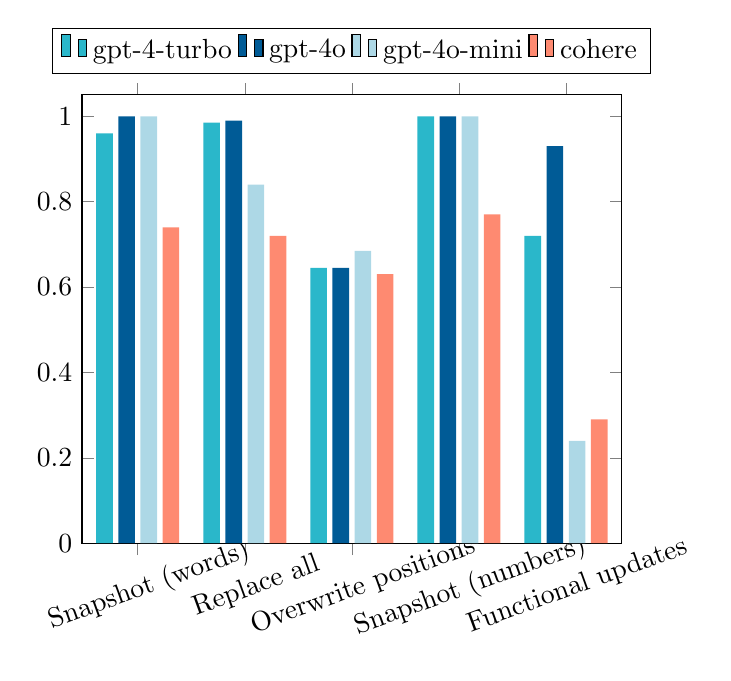
\begin{tikzpicture}
        \begin{axis}[
            ybar,
            bar width=6pt,
            symbolic x coords={Snapshot (words), Replace all, Overwrite positions, Snapshot (numbers), Functional updates},
            xtick=data,
            ymin=0, ymax=1.05,
            legend columns=4,
            legend style={at={(0.5,1.15)}, anchor=north, draw=black},
            enlarge x limits=0.13,
            xticklabel style={rotate=20, anchor=center, yshift=-12pt}
        ]
        
        \addplot[fill={rgb,255:red,42;green,183;blue,202}, draw=none] coordinates {(Snapshot (words),0.96) (Replace all,0.985) (Overwrite positions,0.645) (Snapshot (numbers),1.00) (Functional updates,0.72)};
        \addlegendentry{gpt-4-turbo}
        
        \addplot[fill={rgb,255:red,0;green,91;blue,150}, draw=none] coordinates {(Snapshot (words),1.00) (Replace all,0.99) (Overwrite positions,0.645) (Snapshot (numbers),1.00) (Functional updates,0.93)};
        \addlegendentry{gpt-4o}
        
        \addplot[fill={rgb,255:red,173;green,216;blue,230}, draw=none] coordinates {(Snapshot (words),1.00) (Replace all,0.84) (Overwrite positions,0.685) (Snapshot (numbers),1.00) (Functional updates,0.24)};
        \addlegendentry{gpt-4o-mini}
        
        \addplot[fill={rgb,255:red,254;green,138;blue,113}, draw=none] coordinates {(Snapshot (words),0.74) (Replace all,0.72) (Overwrite positions,0.63) (Snapshot (numbers),0.77) (Functional updates,0.29)};
        \addlegendentry{cohere}
        
        \end{axis}
\end{tikzpicture}}
    \end{subfigure}
    \begin{subfigure}{0.49\columnwidth}
        \resizebox{\textwidth}{!}{    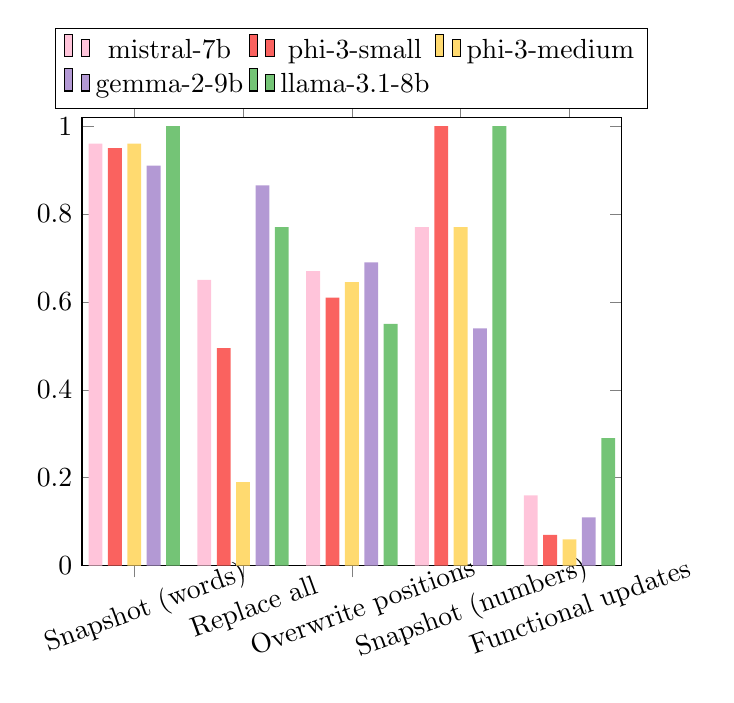
\begin{tikzpicture}
        \begin{axis}[
            ybar,
            bar width=5pt,
            symbolic x coords={Snapshot (words), Replace all, Overwrite positions, Snapshot (numbers), Functional updates},
            xtick=data,
            ymin=0, ymax=1.02,
            legend columns=3,
            legend style={at={(0.5,1.20)}, anchor=north, draw=black},
            enlarge x limits=0.12,
            xticklabel style={rotate=20, anchor=center, yshift=-12pt}
        ]
        
        \addplot[fill={rgb,255:red,255;green,196;blue,218}, draw=none] coordinates {(Snapshot (words),0.96) (Replace all,0.65) (Overwrite positions,0.67) (Snapshot (numbers),0.77) (Functional updates,0.16)};
        \addlegendentry{mistral-7b}
        
        \addplot[fill={rgb,255:red,250;green,98;blue,95}, draw=none] coordinates {(Snapshot (words),0.95) (Replace all,0.495) (Overwrite positions,0.61) (Snapshot (numbers),1.00) (Functional updates,0.07)};
        \addlegendentry{phi-3-small}
        
        \addplot[fill={rgb,255:red,255;green,218;blue,112}, draw=none] coordinates {(Snapshot (words),0.96) (Replace all,0.19) (Overwrite positions,0.645) (Snapshot (numbers),0.77) (Functional updates,0.06)};
        \addlegendentry{phi-3-medium}
        
        \addplot[fill={rgb,255:red,179;green,153;blue,212}, draw=none] coordinates {(Snapshot (words),0.91) (Replace all,0.865) (Overwrite positions,0.69) (Snapshot (numbers),0.54) (Functional updates,0.11)};
        \addlegendentry{gemma-2-9b}
        
        \addplot[fill={rgb,255:red,116;green,196;blue,118}, draw=none] coordinates {(Snapshot (words),1.00) (Replace all,0.77) (Overwrite positions,0.55) (Snapshot (numbers),1.00) (Functional updates,0.29)};
        \addlegendentry{llama-3.1-8b}
        
        \end{axis}
\end{tikzpicture}}
    \end{subfigure}
    \caption{Results for the \textbf{Recall and Edit} tasks.}
    \label{fig:recall}
\end{figure}

\paragraph{Recall and Edit} 
\begin{table}[!h]
    \centering
        \resizebox{0.8\columnwidth}{!}{%
    \begin{tabular}{lllll}
    \toprule
        \textbf{Model} & \textbf{String Search (word)} & \textbf{Snapshot} \\ \hline
gpt-4-turbo    & 1.00 \textcolor{green}{(0.06)} & 1.00 \textcolor{green}{(0.04)} \\ 
gpt-4o         & 1.00 (0.00)                   & 1.00 (0.00)                   \\ 
gpt-4o-mini    & 0.94 \textcolor{red}{(-0.04)}  & 1.00 (0.00)                   \\ 
cohere         & 1.00 (0.00)                   & 1.00 \textcolor{green}{(0.26)} \\ 
mistral-7b     & 1.00 \textcolor{green}{(0.22)} & 0.96 (0.00)                   \\ 
phi-3-small    & 1.00 \textcolor{green}{(0.06)} & 0.99 \textcolor{green}{(0.04)} \\ 
phi-3-medium   & 0.98 \textcolor{red}{(-0.02)}  & 0.87 \textcolor{red}{(-0.09)}  \\ 
gemma-2-9b     & 0.96 \textcolor{red}{(-0.04)}  & 0.96 \textcolor{green}{(0.05)} \\ 
llama-3.1-8b   & 0.98 \textcolor{red}{(-0.02)}  & 1.00 (0.00)                   \\
\bottomrule
    \end{tabular}
    }
    \caption{Ablation study with gibberish context.}
    \label{tab:ablation_gibberish}
\end{table}

Figure \ref{fig:recall} presents the results for the \textbf{Recall and Edit} tasks. While models performed well on basic recall (\textit{Snapshot}), their performance dropped sharply when tasked with making regular edits. A closer analysis of the generated outputs reveals that models struggled with maintaining coherence during edits, often getting trapped in repetitive word loops. For the \textit{Functional Update} task, we deliberately selected simple numerical updates, such as ``Subtract 1 from every number," to ensure the edits were within the models' capabilities. Nevertheless, when comparing performance on \textit{Snapshot (with numbers)} to \textit{Functional Updates}, all models exhibited a steep decline, especially for smaller ones. Analysis of generated outputs revealed that these models frequently deviated from instructions over longer sequences, suggesting difficulties in maintaining consistent rule applications over extended contexts.

Additionally, we conducted a separate ablation study on \textit{Snapshot} and \textit{String Search}. In this study, we replaced meaningful words in the context with gibberish tokens consisting of randomly generated alphabetical characters. As shown in Table \ref{tab:ablation_gibberish}, performance remained largely unchanged, suggesting that semantic meaning was not a significant distractor in these tasks.

\section{Backup: compare with previous works}

\paragraph{Comparison with Theorem 1 of \cite{srikant2024rates}.} While the framework of our proof of Theorem \ref{thm:Srikant-generalize} is mainly inspired by the proof of Theorem 1 of \cite{srikant2024rates}, there are some noteworthy differences. Most importantly, we observe that in the equation beginning from the bottom of Page 7 and continuing to the start of Page 8, the right-most side contains a term
\begin{align}\label{eq:Srikant-error}
-\frac{1}{n-k+1} \mathsf{Tr}\left(\bm{\Sigma}_{\infty}^{-\frac{1}{2}}(\bm{\Sigma}_k - \bm{\Sigma}_{\infty})\bm{\Sigma}_{\infty}^{-\frac{1}{2}}\mathbb{E}[\nabla^2 f(\tilde{\bm{Z}}_k)]\right);
\end{align}
the author argued that ``by taking an expectation to remove conditioning, and defining $\bm{A}_k$ to be $\mathbb{E}[\nabla^2 f(\tilde{\bm{Z}}_k)]$'', this term can be transformed to the term
\begin{align}\label{eq:Srikant-wrong}
-\frac{1}{n-k+1} \mathsf{Tr}\left(\bm{A}_k \left(\bm{\Sigma}_{\infty}^{-\frac{1}{2}} \mathbb{E}[\bm{\Sigma}_k]\bm{\Sigma}_{\infty}^{-\frac{1}{2}}-\bm{I}\right)\right)
\end{align}
in the expression of Theorem 1. However, we note that the function $f(\cdot)$, as defined on Page 6 as the solution to the Stein's equation with respect to $\tilde{h}(\cdot)$, is \emph{dependent on} $\mathcal{F}_{k-1}$; in fact, $f$ corresponds to the function $f_k$ in our proof. Consequently, the terms $\bm{A}_k = \mathbb{E}[\nabla^2 f(\tilde{\bm{Z}}_k)]$ (which is actually a conditional expectation with respect to $\mathcal{F}_{k-1}$), and $\bm{\Sigma}_k$ (which corresponds to $\bm{V}_k$ in our proof), are confounded by $\mathcal{F}_{k-1}$ and hence \emph{not independent}. Therefore, taking expectation, with respect to $\mathcal{F}_0$, on \eqref{eq:Srikant-error} should yield
\begin{align}\label{eq:Srikant-right}
-\frac{1}{n-k+1} \mathbb{E}\left\{\mathsf{Tr}\left(\bm{A}_k \left(\bm{\Sigma}_{\infty}^{-\frac{1}{2}} \bm{\Sigma}_k\bm{\Sigma}_{\infty}^{-\frac{1}{2}}-\bm{I}\right)\right)\right\}
\end{align}
Notice that the expectation is taken over the trace as a whole, instead of only $\bm{\Sigma}_k$. However, also due to the confounding bewteen $\bm{A}_k$ and $\bm{\Sigma}_k$, there is no guarantee that the sum of \eqref{eq:Srikant-right} is bounded as shown in the proof of Theorem 2 in \cite{srikant2024rates} on page 10. In other words, the framework of the proof needs a substantial correction to obtain a meaningful Berry-Esseen bound. 

Our solution in the proof of Theorem \ref{thm:Srikant-generalize} is to replace the matrix $\bm{Q}=\sqrt{n-k+1}\bm{\Sigma}_{\infty}$, as defined on Page 6 of \cite{srikant2024rates}, with the matrix $\bm{P}_k$, following the precedent of \cite{JMLR2019CLT}. This essentially eliminates the term \eqref{eq:Srikant-right}, but would require $\bm{P}_k$ to be measurable with respect to $\mathcal{F}_{k-1}$. For this purpose, we impose the assumption that $\bm{P}_1 = n\bm{\Sigma}_n$ almost surely, also following the precedent of \cite{JMLR2019CLT}. The relaxation of this assumption would be addressed in Theorem \ref{thm:Berry-Esseen-mtg}. 

Another important improvement we made in Theroem \ref{thm:Srikant-generalize} is to tighten the upper bound through a closer scrutiny of the smoothness of the solution to the Stein's equation, as is indicated in Proposition \ref{prop:Stein-smooth}. This paves the way for Corollary \ref{cor:Wu}, the proof of which we present in the next subsection. 


\begin{table}[!htbp] \centering
  \caption{Human Choices and Predictions About GenAI Choice in the Same Problem: Heterogeneity by Exposure and Attitudes (Pooled)}
\begin{adjustbox}{scale=0.8}
\begin{tabular}{@{\extracolsep{5pt}}lccccc}
% \\[-1.8ex]\hline
% \hline \\[-1.8ex]
\toprule
& \multicolumn{5}{c}{\textit{Dependent variable: Prediction}} \
\cr \cline{2-6}
\\[-1.8ex] & \multicolumn{1}{c}{Heavy User} & \multicolumn{1}{c}{Text-Based LLM User} & \multicolumn{1}{c}{Paid User} & \multicolumn{1}{c}{Agree AI Similar} & \multicolumn{1}{c}{Agree AI Better}  \\
\\[-1.8ex] & (1) & (2) & (3) & (4) & (5) \\
% \hline \\[-1.8ex]
\midrule
 X$\times$Heavy User & -0.056$^{}$ & & & & \\
& (0.052) & & & & \\
 X$\times$Text-Based LLM User & & 0.082$^{**}$ & & & \\
& & (0.040) & & & \\
 X$\times$Paid User & & & -0.001$^{}$ & & \\
& & & (0.072) & & \\
 X$\times$Agree AI Similar & & & & 0.033$^{}$ & \\
& & & & (0.045) & \\
 X$\times$Agree AI Better & & & & & 0.019$^{}$ \\
& & & & & (0.017) \\
 Problem FE & Yes & Yes & Yes & Yes & Yes \\
 X$\times$Problem FE & Yes & Yes & Yes & Yes & Yes \\
 G$\times$Problem FE & Yes & Yes & Yes & Yes & Yes \\
% \hline \\[-1.8ex]
\midrule
 Observations & 2700 & 2700 & 2700 & 2700 & 2700 \\
 % Residual Std. Error & 22.874 & 22.851 & 22.863 & 22.847 & 22.895 \\
% \hline
% \hline \\[-1.8ex]
\bottomrule
\textit{Note:} & \multicolumn{5}{r}{Standard errors are clustered at the problem level. $^{*}$p$<$0.1; $^{**}$p$<$0.05; $^{***}$p$<$0.01} \\
% \multicolumn{6}{r}\textit{} \\
\end{tabular}
\end{adjustbox}
\label{tab:group} \end{table}


\paragraph{Match and Compare}
 As shown in Figure \ref{fig:match}, model performance in the \textbf{Match and Compare} tasks was relatively consistent across different model sizes. Given that counting is a well-known weakness in LLMs, it is unsurprising that all models struggled significantly with the counting task, though GPT models performed slightly better than others. However, models generally succeeded in identifying the duplicates (in \textit{Find duplicates}), and primarily struggled with the counting aspect -- which requires tracking and updating an integer state, a skill that is more similar to stateful processing. This suggests that relying solely on counting-based tests \cite{song2024countingstars} could overly bias the evaluation and fail to capture broader model capabilities. The results also indicate that models exhibit some ability to recognize relative positions and group associations, but their accuracy remains limited (ranging between 0.6-0.8). A closer examination of model generations reveals an overwhelming tendency for the models to produce false positive errors -- models often answer “yes” when the correct answer is “no”, while making very few false negative errors. This means that when the relationship is correct, the models can more reliably identify it. This may stem from a combination of their inherent inclination to agree and the difficulty in recognizing relative comparisons and associations.

% \begin{figure}[h]
%     \centering
%     \includegraphics[width=0.92\columnwidth]{images/difference.png}
%     \caption{Results for \textbf{Spot the Differences }tasks.}
%     \label{fig:difference}
% \end{figure}

\begin{figure}[h]
\centering
\resizebox{0.9\columnwidth}{!}{
 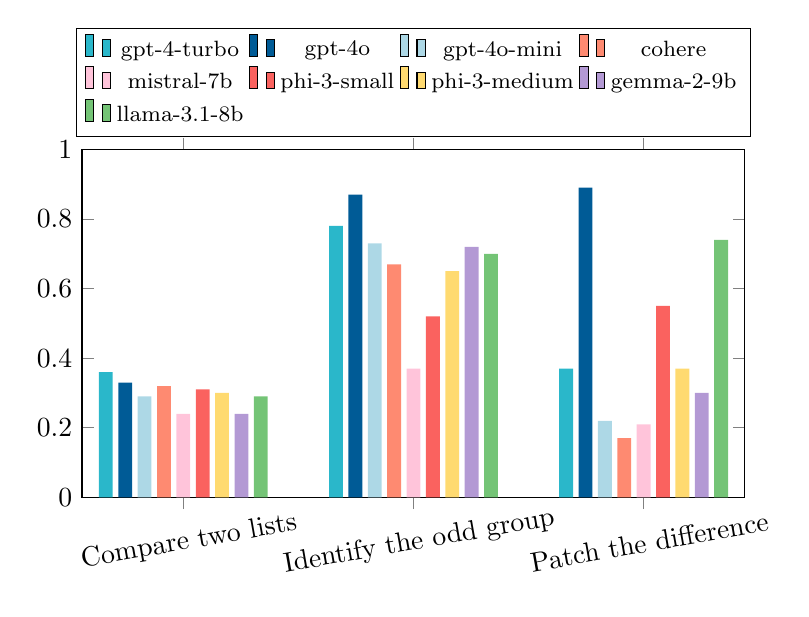
\begin{tikzpicture}
        \begin{axis}[
            ybar,
            bar width=5pt,
            symbolic x coords={Compare two lists, Identify the odd group, Patch the difference},
            xtick=data,
            ymin=0, ymax=1.0,
            legend columns=4,
            legend style={at={(0.5,1.35)}, anchor=north, draw=black, font=\footnotesize},
            enlarge x limits=0.22,
            xticklabel style={rotate=10, anchor=center, yshift=-12pt},
            width=10cm, height=6cm,
        ]
        
        \addplot[fill={rgb,255:red,42;green,183;blue,202}, draw=none] coordinates {(Compare two lists,0.36) (Identify the odd group,0.78) (Patch the difference,0.37)};
        \addlegendentry{gpt-4-turbo}
        
        \addplot[fill={rgb,255:red,0;green,91;blue,150}, draw=none] coordinates {(Compare two lists,0.33) (Identify the odd group,0.87) (Patch the difference,0.89)};
        \addlegendentry{gpt-4o}
        
        \addplot[fill={rgb,255:red,173;green,216;blue,230}, draw=none] coordinates {(Compare two lists,0.29) (Identify the odd group,0.73) (Patch the difference,0.22)};
        \addlegendentry{gpt-4o-mini}
        
        \addplot[fill={rgb,255:red,254;green,138;blue,113}, draw=none] coordinates {(Compare two lists,0.32) (Identify the odd group,0.67) (Patch the difference,0.17)};
        \addlegendentry{cohere}
        
        \addplot[fill={rgb,255:red,255;green,196;blue,218}, draw=none] coordinates {(Compare two lists,0.24) (Identify the odd group,0.37) (Patch the difference,0.21)};
        \addlegendentry{mistral-7b}
        
        \addplot[fill={rgb,255:red,250;green,98;blue,95}, draw=none] coordinates {(Compare two lists,0.31) (Identify the odd group,0.52) (Patch the difference,0.55)};
        \addlegendentry{phi-3-small}
        
        \addplot[fill={rgb,255:red,255;green,218;blue,112}, draw=none] coordinates {(Compare two lists,0.30) (Identify the odd group,0.65) (Patch the difference,0.37)};
        \addlegendentry{phi-3-medium}
        
        \addplot[fill={rgb,255:red,179;green,153;blue,212}, draw=none] coordinates {(Compare two lists,0.24) (Identify the odd group,0.72) (Patch the difference,0.30)};
        \addlegendentry{gemma-2-9b}
        
        \addplot[fill={rgb,255:red,116;green,196;blue,118}, draw=none] coordinates {(Compare two lists,0.29) (Identify the odd group,0.70) (Patch the difference,0.74)};
        \addlegendentry{llama-3.1-8b}
        
        \end{axis}
    \end{tikzpicture}}
    \caption{Results for \textbf{Spot the Differences }tasks.}
    \label{fig:difference}
\end{figure}

\paragraph{Spot the Differences}
As shown in Figure \ref{fig:difference}, performance across all models are poor on \textit{Compare Two Lists}, suggesting inherent difficulties in cross-referencing information across long contexts, even for larger models.  GPT-4o and the LLaMA model significantly outperform the others in the \textit{Identify the Odd Group} task, highlighting a general weakness in detecting contextual differences by the other models. However, an 8B LLaMA model outperforms both equivalently-sized models and even GPT-4 in this task, suggesting that model size alone was not the determining factor. This indicates that architectural differences, training objectives, or specific inductive biases may contribute to improved performance in comparative memory utilization.


\paragraph{Compute on Sets and Lists}
The tasks in this category require models to recognize and process group structures within the context, and performance gradually declines as the complexity of the task increases (see Table \ref{tab:lists}). For instance, in comparing the \textit{Group Membership} task with the \textit{String Search} task, where the former requires identifying which list a word belongs to rather than simply determining its presence, the performance of open-source models drops considerably. Similarly, in comparing the \textit{Group Association} task with the \textit{Group Membership} task, where the former requires determining whether two words belong to the same group, all models exhibit a noticeable decline in performance. The decline becomes even more pronounced when comparing the \textit{ Group Association (alternating)} variant of the task to the standard \textit{Group Association} task. Here, the context involves alternating repeated groups rather than simple group structures, which further challenges the models' abilities to handle partitioned contexts effectively.

An interesting observation was found during the \textit{Iterate} task. In an ablation study, we modified the task to require returning the first words in each list instead of the last words (making it more similar to the \textit{Batch Search} task). The performance sharply declines when models are asked to return the last words, despite their strong information-fetching capabilities. This suggests that, while the models can retrieve information effectively, they struggle to accurately recognize and process partitions within the context.


\begin{table}[h!]
\large
\centering
\begin{adjustbox}{width=\columnwidth} % Automatically fit within column width
\begin{tabular}{|c|p{0.75\columnwidth}|} % Adjust the second column width proportionally
\hline
\textbf{Symbol} & \textbf{Explanation} \\ \hline
$q^{\text{obj}} \in SE(2)$ & Object pose \\ \hline
$q^{\text{robot}} \in \mathbb{R}^9$ & Robot configuration (9 DoF robot joint position) \\ \hline
$q^{\text{obj}}_\text{sg} \in SE(2)$ & Subgoal object pose \\ \hline
$q^{\text{robot}}_\text{sg} \in SE(3) \times \mathbb{R}^3$ & Subgoal robot configuration (End-effector pose in $SE(3)$ and gripper tip positions in 3D space) \\ \hline
$q^{\text{obj}}_{\text{init}} \in SE(2)$ & Initial object pose of the task \\ \hline
$q^{\text{robot}}_{\text{init}} \in \mathbb{R}^9$ & Initial robot configuration of the task (9 DoF robot joint position) \\ \hline
$q^{\text{obj}}_{\text{goal}} \in SE(2)$ & Goal object pose of the task \\ \hline
$s$ & State \\ \hline
% $sg$ & Subgoal information (e.g., subgoal object pose, robot configuration) \\ \hline
\end{tabular}
\end{adjustbox}
\caption{Notation table for task parameters}
\label{tab:state_notation}
\end{table}

\paragraph{Stateful Processing}

\begin{figure}[t!]
    \centering
    \begin{subfigure}{0.49\columnwidth}
        \resizebox{\textwidth}{!}{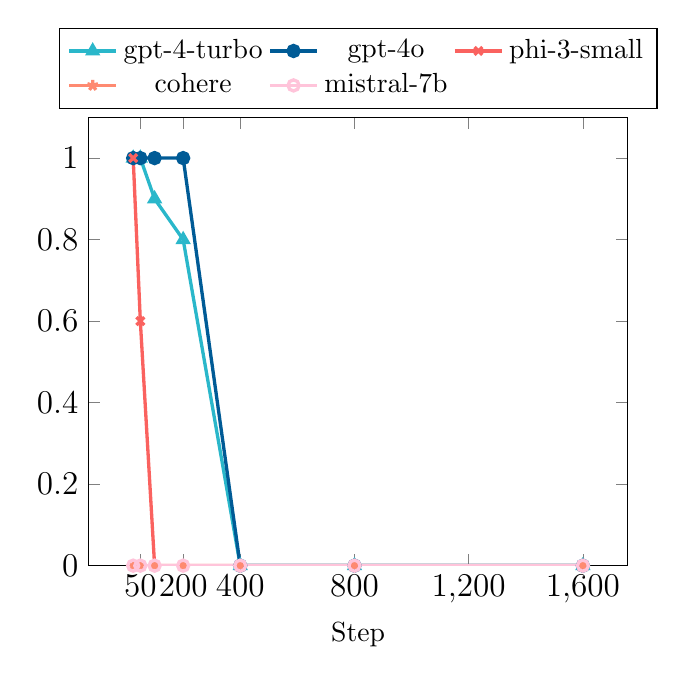
\begin{tikzpicture}
    \begin{axis}[
        xlabel={Step},
        legend style={at={(0.5,1.2)}, anchor=north, cells={align=left}, legend columns=3},
        ymin=0, ymax=1.1,
        xtick={50, 200, 400, 800, 1200, 1600},
        ytick={0,0.2,0.4,0.6,0.8,1.0},
        grid=none,
        tick label style={font=\large}
    ]

    % GPT-4-Turbo
    \addplot[mark=triangle, very thick, color={rgb,255:red,42;green,183;blue,202}] coordinates {
        (25,1.0) (50,1.0) (100,0.9) (200,0.8) (400,0.0) (800,0.0) (1600,0.0)
    };
    \addlegendentry{gpt-4-turbo}

    % GPT-4o
    \addplot[mark=*, very thick, color={rgb,255:red,0;green,91;blue,150}] coordinates {
        (25,1.0) (50,1.0) (100,1.0) (200,1.0) (400,0.0) (800,0.0) (1600,0.0)
    };
    \addlegendentry{gpt-4o}



    % Phi-3-Small
    \addplot[mark=x, very thick, color={rgb,255:red,250;green,98;blue,95}] coordinates {
        (25,1.0) (50,0.6) (100,0.0) (200,0.0) (400,0.0) (800,0.0) (1600,0.0)
    };
    \addlegendentry{phi-3-small}

    % Cohere
    \addplot[mark=star, very thick, color={rgb,255:red,254;green,138;blue,113}] coordinates {
        (25,0.0) (50,0.0) (100,0.0) (200,0.0) (400,0.0) (800,0.0) (1600,0.0)
    };
    \addlegendentry{cohere}

    % Mistral-7B
    \addplot[mark=o, very thick, color={rgb,255:red,255;green,196;blue,218}] coordinates {
        (25,0.0) (50,0.0) (100,0.0) (200,0.0) (400,0.0) (800,0.0) (1600,0.0)
    };
    \addlegendentry{mistral-7b}
    
    \end{axis}
\end{tikzpicture}}
    \end{subfigure}
    \begin{subfigure}{0.49\columnwidth}
        \resizebox{\textwidth}{!}{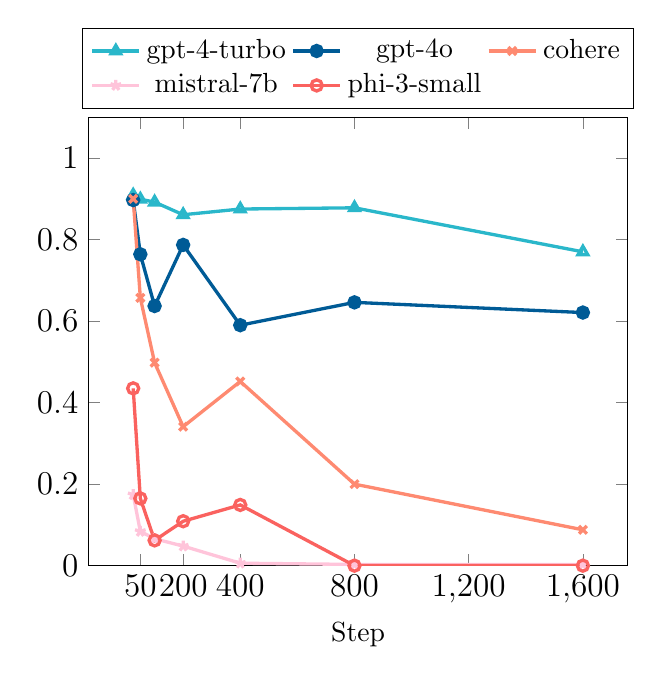
\begin{tikzpicture}
    \begin{axis}[
        xlabel={Step},
        legend style={at={(0.5,1.2)}, anchor=north, cells={align=left}, legend columns=3},
        ymin=0, ymax=1.1,
        xtick={50, 200, 400, 800, 1200, 1600},
        ytick={0,0.2,0.4,0.6,0.8,1.0},
        grid=none,
        tick label style={font=\large}
    ]

    % GPT-4-Turbo
    \addplot[mark=triangle, very thick, color={rgb,255:red,42;green,183;blue,202}] coordinates {
        (25,0.909) (50,0.899) (100,0.892) (200,0.861) (400,0.875) (800,0.878) (1600,0.770)
    };
    \addlegendentry{gpt-4-turbo}

    % GPT-4o
    \addplot[mark=*, very thick, color={rgb,255:red,0;green,91;blue,150}] coordinates {
        (25,0.897) (50,0.764) (100,0.637) (200,0.787) (400,0.590) (800,0.646) (1600,0.621)
    };
    \addlegendentry{gpt-4o}

    % Cohere
    \addplot[mark=x, very thick, color={rgb,255:red,254;green,138;blue,113}] coordinates {
        (25,0.900) (50,0.657) (100,0.498) (200,0.341) (400,0.452) (800,0.200) (1600,0.088)
    };
    \addlegendentry{cohere}

    % Mistral-7B
    \addplot[mark=star, very thick, color={rgb,255:red,255;green,196;blue,218}] coordinates {
        (25,0.174) (50,0.084) (100,0.066) (200,0.048) (400,0.006) (800,0.003) (1600,0.003)
    };
    \addlegendentry{mistral-7b}

    % Phi-3-Small
    \addplot[mark=o, very thick, color={rgb,255:red,250;green,98;blue,95}] coordinates {
        (25,0.435) (50,0.165) (100,0.062) (200,0.109) (400,0.149) (800,0.000) (1600,0.000)
    };
    \addlegendentry{phi-3-small}
    
    \end{axis}
\end{tikzpicture}}
    \end{subfigure}
    \caption{Ablation study on the number of operation steps for the \textbf{quantity state} (left) and\textbf{ set state }(right).}
    \label{fig:ablation_state_step}
\end{figure}



Table \ref{tab:state} presents the results for the \textbf{Stateful Processing} tasks, where performance gaps among models are the most pronounced. The GPT-4(o) models perform well on integer state tracking, while most other models struggle (near zero accuracy). For set state tracking, larger models generally perform better.

We conducted an ablation study to examine how the number of operation steps influences performance of five selected models (Fig. \ref{fig:ablation_state_step}). For quantity state tracking, GPT-4(o) models perform well within fewer than 200 steps but experience a sharp decline in accuracy beyond this threshold. For set state tracking, the performance decline is more gradual. The differences in performance drop between the two tasks can be attributed to the nature of the two tasks. While tracking an integer state might seem simpler than tracking a set, it actually requires the model to maintain and apply every operation sequentially to compute the final value. In contrast, for set state, the fixed size of the set makes more recent operations more relevant to the final state, reducing the need for exhaustive step-by-step tracking. Nevertheless, even in this scenario, all models show a clear inability to handle longer or more complex operation sequences effectively. Interestingly, GPT-4 model outperformed GPT-4o at this task, suggesting potential optimization trade-offs may have affected its ability to manage set-based updates. 

Overall, while larger models like GPT-4(o) exhibit some ability to track state over time, their effectiveness rapidly deteriorates as task complexity increases. Smaller models, in particular, struggle to track operations over time, pointing to significant gaps in their ability to manage and process sequential dependencies critical for state tracking tasks.

\subsection{Results on Composite Tests}

\section{Simple Construction of Projective Compositions}
\label{sec:comp_coord}

It is not clear apriori that projective compositional distributions satisfying Definition \ref{def:proj_comp} ever exist, much less that there is any straightforward way to sample from them.
To explore this, we first restrict attention to perhaps the simplest setting, where the projection functions $\{\Pi_i\}$ are
just coordinate restrictions.
This setting is meant to generalize the intuition we had
in the CLEVR example of Figure~\ref{fig:len_gen},
where different objects were composed in disjoint regions of the image.
We first define the construction of the composed distribution,
and then establish its theoretical properties.








\subsection{Defining the Construction}
Formally, suppose we have a set of distributions
$(p_1, p_2, \ldots, p_k)$ that we wish to compose;
in our running CLEVR example, each $p_i$ is the distribution of images
with a single object at position $i$.
Suppose also we have some reference distribution $p_b$,
which can be arbitrary, but should be thought of as a 
``common background'' to the $p_i$s.
Then, one popular way to construct a composed distribution
is via the \emph{compositional operator} defined below.
(A special case of this construction is used in \citet{du2023reduce}, for example).


\begin{definition}[Composition Operator]
    \label{def:comp_oper}
    Define the \emph{composition operator} $\cC$ acting on an arbitrary set of distributions $(p_b, p_1, p_2, \ldots)$ by
    \begin{align}
    \label{eq:comp_oper}
    \cC[\vec{p}] := \cC[p_b, p_1, p_2, \dots](x) := \frac{1}{Z} p_b(x) \prod_i \frac{p_i(x)}{p_b(x)},
    \end{align}
    where $Z$ is the appropriate normalization constant. We name $\cC[\vec{p}]$ the \emph{composed distribution}, and the score of $\cC[\vec{p}]$ the \emph{compositional score}:
    \begin{align}
    \label{eqn:comp_score}
    &\grad_x \log \cC[\vec{p}](x)  \\
    &= \grad_x \log p_b(x) + \sum_i \left( \grad_x \log p_i(x) - \grad_x \log p_b(x) \right). \notag
    \end{align}
\end{definition}
Notice that if $p_b$ is taken to be the unconditional distribution then this is exactly the Bayes-composition.


\vspace{-0.5em}
\subsection{When does the Composition Operator Work?}
We can always apply the composition operator to any set of distributions,
but when does this actually yield a ``correct'' composition
(according to Definition~\ref{def:proj_comp})?
One special case is when each distribution $p_i$ is
``active'' on a different, non-overlapping set of coordinates.
We formalize this property below
as \emph{Factorized Conditionals} (Definition~\ref{def:factorized}).
The idea is, 
each distribution $p_i$
must have a particular set of ``mask'' coordinates $M_i \subseteq [n]$ which it
samples in a characteristic way,
while independently sampling all other coordinates
from a common background distribution.
If a set of distributions $(p_b, p_1, p_2, \ldots)$ has this
\emph{Factorized Conditional} structure, then 
the composition
operator will produce a projective composition (as we will prove below).



\begin{definition}[Factorized-Conditionals]
\label{def:factorized}

We say a set of distributions $(p_b, p_1, p_2, \dots p_k)$
over $\R^n$
are \emph{Factorized Conditionals} if
there exists a partition of coordinates $[n]$
into disjoint subsets $M_b, M_1, \dots M_k$ such that:
\begin{enumerate}
    \setlength{\itemsep}{1pt}
    \item $(x|_{M_i}, x|_{M_i^c})$ are independent under $p_i$.
    \item $(x|_{M_b}, x|_{M_1}, x|_{M_2}, \dots, x|_{M_k})$
    are mutually independent under $p_b$.
    \item $p_i(x|_{M_i^c}) = p_b(x|_{M_i^c})$.
\end{enumerate}

Equivalently, if we have:
\begin{align}
    p_i(x) &= p_i(x|_{M_i}) p_b(x|_{M_i^c}), \text{ and} \label{eqn:cc-cond}\\
    p_b(x) &= p_b(x|_{M_b}) \prod_{i \in [k]} p_b(x|_{M_i}). \notag
\end{align}
\end{definition}
\vspace{-1em}
Equation~\eqref{eqn:cc-cond} means that each $p_i$
can be sampled by first sampling $x \sim p_b$,
and then overwriting the coordinates of $M_i$
according to some other distribution (which can be specific to distribution $i$).
For instance, the experiment of Figure~\ref{fig:len_gen}
intuitively satisfies this property, since 
each of the conditional distributions could essentially be sampled
by first sampling an empty background image ($p_b$), then ``pasting''
a random object in the appropriate location (corresponding to pixels $M_i$).
If a set of distributions obey this Factorized Conditional structure,
then we can prove that the composition operator $\cC$
yields a correct projective composition,
and reverse-diffusion correctly samples from it.
Below, let $N_t$ denote the noise operator of the
diffusion process\footnote{Our results are agnostic to the specific diffusion noise-schedule and scaling used.} at time $t$.

\begin{theorem}[Correctness of Composition]
\label{lem:compose}
Suppose a set of distributions $(p_b, p_1, p_2, \dots p_k)$
satisfy Definition~\ref{def:factorized},
with corresponding masks $\{M_i\}_i$.
Consider running the reverse-diffusion SDE 
using the following compositional scores at each time $t$:
\begin{align}
s_t(x_t) &:= \grad_x \log \cC[p_b^t, p_1^t, p_2^t, \ldots](x_t),
\end{align}
where $p_i^t := N_t[p_i]$ are the noisy distributions.
Then, the distribution of the generated sample $x_0$ at time $t=0$ is:
\begin{align}
\label{eqn:p_hat}
\hat{p}(x) := p_b(x|_{M_b}) \prod_i p_i(x|_{M_i}).
\end{align}
In particular,
$\hat{p}(x|_{M_i}) = p_i(x|_{M_i})$ for all $i$,
and so
$\hat{p}$ is a projective composition
with respect to projections $\{\Pi_i(x) := x|_{M_i}\}_i$,
per Definition \ref{def:proj_comp}.
\end{theorem}




Unpacking this, Line \ref{eqn:p_hat} says that the final generated distribution
$\hat{p}(x)$ can be sampled by
first sampling
the coordinates $M_b$ according to $p_b$ (marginally),
then independently sampling 
coordinates $M_i$ according to $p_i$ (marginally) for each $i$.
Similarly, by assumption, $p_i(x)$ can be sampled by first sampling the coordinates $M_i$ in some specific way, and then independently sampling the remaining coordinates according to $p_b$. Therefore Theorem \ref{lem:compose} says that $\hat{p}(x)$ samples the coordinates \emph{$M_i$ exactly as they would be sampled by $p_i$}, for each $i$ we wish to compose. 

\begin{proof}(Sketch) \small
Since $\vec{p}$ satisfies Definition \ref{def:factorized}, we have
\begin{align*}
&\cC[\vec{p}](x) := p_b(x) \prod_i \frac{p_i(x)}{p_b(x)} \notag 
= p_b(x) \prod_i \frac{p_b(x_t|_{M_i^c}) p_i(x|_{M_i})}{p_b(x|_{M_i^c})p_b(x|_{M_i})} \notag \\
&= p_b(x) \prod_i \frac{p_i(x|_{M_i})}{p_b(x|_{M_i})} \notag 
= p_b(x|_{M_b}) \prod_i p_i(x_t|_{M_i}) := \hat{p}(x).
\end{align*}
The sampling guarantee follows from the commutativity of composition with the diffusion noising process, i.e. $\cC[\vec{p^t}]= N_t[\cC[\vec{p}]]$. 
The complete proof is in Appendix \ref{app:compose_pf}.
\end{proof}

\begin{remark}
In fact, Theorem~\ref{lem:compose} still holds under any orthogonal transformation of the variables,
because the diffusion noise process commutes with orthogonal transforms.
We formalize this as Lemma~\ref{lem:orthogonal_sampling}.
\end{remark}

\begin{remark}
Compositionality is often thought of in terms of orthogonality between scores.
Definition \ref{def:factorized} implies orthogonality between the score differences that appear in the composed score \eqref{eqn:comp_score}:
$\grad_x \log p_i^t(x_t) - \grad_x \log p_b^t(x_t),$
but the former condition is strictly stronger
(c.f. Appendix \ref{app:score_orthog}).
\end{remark}

\begin{remark}
Notice that the composition operator $\cC$
can be applied to a set of Factorized Conditional
distributions
without knowing the coordinate partition $\{M_i\}$.
That is, we can compose distributions and compute scores
without knowing apriori exactly ``how'' these distributions are supposed to compose
(i.e. which coordinates $p_i$ is active on).
This is already somewhat remarkable, and we will see a much
stronger version of this property in the next section.
\end{remark}

\textbf{Importance of background.}
Our derivations highlight the crucial role of the background
distribution $p_b$ for the composition operator  
(Definition~\ref{def:comp_oper}).
While prior works have taken $p_b$ to be an unconditional distribution and the $p_i$'s its associated conditionals,
our results suggest this is not always the optimal choice -- in particular,
it may not satisfy a Factorized Conditional structure (Definition~\ref{def:factorized}). Figure~\ref{fig:len_gen_monster} demonstrates this empirically: settings (a) and (b) attempt to compose the same distributions using different backgrounds -- empty (a) or unconditional (b) -- with very different results.

\subsection{Approximate Factorized Conditionals in CLEVR.}
\label{sec:clevr-details}

In \cref{fig:len_gen_monster} we explore compositional length-generalization (or lack thereof) in three different setting, two of which (\cref{fig:len_gen_monster}a and \ref{fig:len_gen_monster}c) approximately satisfy \cref{def:factorized}. In this section we explicitly describe how our definition of Factorized Conditionals approximately captures the CLEVR settings of Figures \ref{fig:len_gen_monster}a and \ref{fig:len_gen_monster}c. The setting of \ref{fig:len_gen_monster}b does not satisfy our conditions, as discussed in \cref{sec:problematic-compositions}.

\textbf{Single object distributions with empty background.}
This is the setting of both \cref{fig:len_gen} and \cref{fig:len_gen_monster}a.
The background distribution $p_b$ 
over $n$ pixels is images of an empty scene with no objects.
For each $i \in \{1,\ldots,L\}$ (where $L=4$ in \cref{fig:len_gen} and $L=9$ in \cref{fig:len_gen_monster}a), define the set $M_i \subset [n]$ 
as the set of pixel indices surrounding location $i$.
($M_i$ should be thought of as a ``mask'' that
that masks out objects at location $i$).
Let $M_b := (\cup_i M_i)^c$ be the remaining
pixels in the image.
Then, we claim the distributions $(p_b, p_1, \ldots, p_L)$
form approximately
Factorized Conditionals, with corresponding
coordinate partition $\{M_i\}$.
This is essentially because each distribution $p_i$
matches the background $p_b$ on all pixels except those surrounding
location $i$ (further detail in Appendix~\ref{app:clevr-details}).
Note, however, that the conditions of Definition~\ref{def:factorized}
do not \emph{exactly} hold in the experiment of Figure~\ref{fig:len_gen} -- there is still some dependence between
the masks $M_i$, since objects can cast shadows or even occlude each other.
Empirically, these deviations 
have greater impact
when composing many objects, as seen in \cref{fig:len_gen_monster}a.


\textbf{Bayes composition with cluttered distributions.}
In \cref{fig:len_gen_monster}c we replicate CLEVR experiments in  \citet{du2023reduce, liu2022compositional} where the images contain many objects (1-5) and the conditions label the location of one randomly-chosen object. It turns out the unconditional together with the conditionals can approximately act as Factorized Conditionals in ``cluttered'' settings like this one. The intuition is that if the conditional distributions each contain one specific object plus many independently sampled random objects (``clutter''), then the unconditional distribution \emph{almost} looks like independently sampled random objects, which together with the conditionals \emph{would} satisfy Definition \ref{def:factorized} (further discussion in Appendix \ref{app:clevr-details} and \ref{app:bayes_connect}). This helps to explain the length-generalization observed in \citet{liu2022compositional} and verified in our experiments (\cref{fig:len_gen_monster}c).







\section{Projective Composition in Feature Space}
\label{sec:comp_feature}

\begin{figure}
    \centering
    \includegraphics[width=1.0\linewidth]{figures/feat-space-vis.png}
    \caption{A commutative diagram illustrating Theorem~\ref{lem:transform_comp}.
    Performing composition in pixel space is equivalent 
    to encoding into a feature space ($\cA$),
    composing there,
    and decoding back
    to pixel space ($\cA^{-1}$).
    }
    \label{fig:feat-space-vis}
\end{figure}

So far we have focused on the setting where the projection functions $\Pi_i$ are simply projections onto coordinate subsets $M_i$ in the native space (e.g. pixel space).
This covers simple examples like Figure~\ref{fig:len_gen} but does not include more realistic situations such as Figure~\ref{fig:style-content},
where the properties to be composed are more abstract.
For example a property like ``oil painting'' does not correspond to projection
onto a specific subset of pixels in an image.
However, we may hope that there exists some conceptual feature space
in which ``oil painting'' does correspond to a particular subset of variables.
In this section, we extend our results to the case where the composition occurs in some conceptual feature space, and each distribution to be composed
corresponds to some particular subset of \emph{features}.


Our main result is a featurized analogue of Theorem~\ref{lem:compose}:
if there exists \emph{any} invertible transform $\cA$
mapping into a feature space
where Definition \ref{def:factorized} holds,
then the composition operator (Definition~\ref{def:comp_oper})
yields a projective composition in this feature space, as shown in Figure~\ref{fig:feat-space-vis}.

\begin{theorem}[Feature-space Composition]
\label{lem:transform_comp}
Given distributions $\vec{p} := (p_b, p_1, p_2, \dots p_k)$,
suppose there exists a diffeomorphism $\cA: \R^n \to \R^n$
such that
$(\cA \sharp p_b, \cA \sharp p_1, \dots \cA \sharp p_k)$
satisfy Definition~\ref{def:factorized},
with corresponding partition $M_i \subseteq [n]$.
Then, the composition $\hat{p} := \cC[\vec{p}]$ satisfies:
\begin{align}
\label{eqn:p_hat_A}
\cA \sharp \hat{p}(z)
\equiv
(\cA \sharp p_b (z))|_{M_b} \prod_{i=1}^k (\cA \sharp p_i(z))|_{M_i}.
\end{align}
Therefore, $\hat{p}$
is a projective composition of $\vec{p}$ w.r.t. projection functions
$\{\Pi_i(x) := \cA(x)|_{M_i}\}$.
\end{theorem}
This theorem is remarkable because it means we can
compose distributions $(p_b, p_1, p_2, \dots)$ in the base space,
and this composition will ``work correctly'' in the feature space
automatically (Equation~\ref{eqn:p_hat_A}),
without us ever needing to compute or even know the feature transform $\cA$
explicitly.



Theorem~\ref{lem:transform_comp} may apriori seem too strong
to be true, since it somehow holds for all feature spaces $\cA$
simultaneously.
The key observation underlying Theorem~\ref{lem:transform_comp} 
is that the composition operator $\cC$ behaves
well under reparameterization.
\begin{lemma}[Reparameterization Equivariance]
\label{lem:reparam}
The composition operator of Definition~\ref{def:comp_oper}
is reparameterization-equivariant. That is,
for all diffeomorphisms $\cA: \R^n \to \R^n$
and all tuples of distributions $\vec{p} = (p_b, p_1, p_2, \dots, p_k)$,
\begin{align}
 \cC[ \cA \sharp \vec{p}] =  \cA \sharp \cC[\vec{p}].
\end{align}
\end{lemma}
\arxiv{\footnote{
For example (separate from our goals in this paper):
Classifier-Free-Guidance can be seen as an instance of the composition operator.
Thus, Lemma~\ref{lem:reparam} implies that performing CFG
in latent space is \emph{equivalent} to CFG in pixel-space,
assuming accurate score-models in both cases.}}
\arxiv{This lemma is potentially of independent interest:
reparametrization-equivariance
is a very strong property which is typically not satisfied by
standard operations between probability distributions---
for example, the ``simple product'' $p_1(x)p_2(x)$ does not satisfy it---
so it is mathematically notable that the composition operator 
has this structure.
Lemma~\ref{lem:reparam} and Theorem~\ref{lem:transform_comp}
are proved in Appendix \ref{app:param-indep}.}

This lemma is potentially of independent interest:
equivariance distinguishes the composition operator
from many other common operators
(e.g. the simple product).
Lemma ~\ref{lem:reparam} and Theorem~\ref{lem:transform_comp}
are proved in Appendix \ref{app:param-indep}.

\section{Sampling from Compositions.}
The feature-space Theorem~\ref{lem:transform_comp} is weaker than Theorem~\ref{lem:compose}
in one important way: it does not provide a sampling algorithm.
That is, Theorem~\ref{lem:transform_comp} guarantees that $\hat{p} := \cC[\vec{p}]$
is a projective composition, but does not guarantee that reverse-diffusion
is a valid sampling method.

There is one special case where diffusion sampling \emph{is} guaranteed to work, namely, for orthogonal transforms (which can seen as a straightforward extension of the coordinate-aligned case of \cref{lem:compose}):
\begin{lemma}[Orthogonal transform enables diffusion sampling]
\label{lem:orthogonal_sampling}
If the assumptions of Lemma \ref{lem:transform_comp} hold for $\cA(x) = Ax$, where $A$ is an orthogonal matrix, then running a reverse diffusion sampler with scores $s_t = \grad_x \log \cC[\vec{p}^t]$ generates the composed distribution $\hat{p} = \cC[\vec{p}]$ satisfying \eqref{eqn:p_hat_A}.
\end{lemma}
The proof is given in \cref{app:orthog_sample_pf}.

However, for general invertible transforms, we have no such sampling guarantees.
Part of this is inherent: in the feature-space setting, the 
diffusion noise operator $N_t$ no longer commutes
with the composition operator $\cC$ in general,
 so scores of the noisy composed 
distribution $N_t[\cC[\vec{p}]]$
cannot be computed from scores
of the noisy base distributions $N_t[\vec{p}]$.
Nevertheless, one may hope to sample from the distribution $\hat{p}$
using other samplers besides diffusion, 
such as annealed Langevin Dynamics
or
Predictor-Corrector methods \citep{song2020score}.
We find that the situation is surprisingly subtle:
composition $\cC$ produces distributions which
are in some cases easy to sample (e.g. with diffusion),
yet in other cases apparently hard to sample.
For example, in the
setting of Figure~\ref{fig:clevr_color_comp}, 
our Theorem~\ref{lem:transform_comp} implies
that all pairs of colors should compose equally well
at time $t=0$, since there exist diffeomorphisms
(indeed, linear transforms) between different colors.
However, as we saw,
the diffusion sampler
fails to sample from compositions 
of non-orthogonal colors--- and 
empirically, even more sophisticated
samplers such as Predictor-Correctors
also fail in this setting.
At first glance, it may seem odd that
composed distributions are so hard to sample,
when their constituent distributions are relatively easy to sample.
One possible reason for this below is that the composition operator has extremely poor Lipchitz constant,
so it is possible for a set of distributions $\vec{p}$ to ``vary smoothly''
(e.g. diffusing over time) while their composition $\cC[\vec{p}]$
changes abruptly.
We formalize this in \cref{lem:lipschitz} (further discussion and proof in Appendix \ref{app:lipschitz}).
\begin{lemma}[Composition Non-Smoothness]
\label{lem:lipschitz}
For any set of distributions $\{p_b, p_1, p_2, \dots, p_k\}$,
and any noise scale $t := \sigma$,
define the noisy distributions 
$p_i^t := N_{t}[p_i]$,
and let $q^t$ denote the composed distribution at time $t$: $q^t := \cC[\vec{p}^t]$. Then, for any choice of $\tau > 0$,
there exist distributions $\{p_b, p_1, \dots p_k\}$ over $\R^n$
such that
\begin{enumerate}
    \setlength{\itemsep}{0pt}
    \item For all $i$, the annealing path of $p_i$ is 
    $\cO(1)$-Lipshitz:
    $\forall t, t': W_2(p_i^{t}, p_i^{t'}) \leq \cO(1) |t - t'|$.
    \item The annealing path of $q$ has Lipshitz constant
    at least $\Omega(\tau^{-1})$:
    $\exists t, t': W_2(q^{t}, q^{t'}) \geq \frac{|t - t'|}{2\tau}.$
\end{enumerate}
\end{lemma}




The composite tests significantly challenge the models by combining multiple atomic capabilities into a single test. In the \textit{Processing Data Blocks} task, the context is fixed at 4k tokens, while for the \textit{Theory of Mind} task, the number of operation steps is set to 100. As shown in Table \ref{tab:comp}, model performance on both tasks are generally low, showing a broad inability to handle the more complex scenarios. Performance across all models drop substantially on composite tasks compared to their performance on individual capability tasks, such as search, recall, and group processing. 

Interestingly, some smaller models, like Mistral and Phi-3-small, exhibit slightly better performance on the \textit{Theory of Mind} task than on the set state tracking task. This anomaly likely stems from their already weak state tracking ability, which limits their performance across both tasks. Additionally, these models tend to generate longer answers in the set state task which reduces the set overlap.

Notably, even the most capable models, such as GPT-4-turbo and GPT-4o, struggle, showing that scaling model size alone is not enough for solving these composite tasks. Additionally, the variation in performance among smaller models suggests that their limitations stem not only from size but also from underlying architectural or training differences. This indicates that smaller models require more targeted care to bridge the gap in effective memory use.



% \section{Research Questions}
% \label{sec:rq}

% Introduce your research questions briefly
\setlength{\parskip}{0pt}

\section{Quantitaive Analysis}
\label{sec:study}



% Please add the following required packages to your document preamble:
% \usepackage{booktabs}
\begin{table}[]
\caption{Pass@1 (\%) scores for various SOTA LLMs on DS-1000 and \tool.}
\label{tab:RQ1_ACC}
\center
\resizebox{0.6\linewidth}{!}{
\begin{tabular}{llr}
\toprule
\textbf{Benchmark}                                      & \textbf{LLM}              & \textbf{Pass@1} \\ 
\midrule
\multirow{4}{*}{DS-1000}& GPT-4o           & 60\\
 & Claude 3.5 sonnet&54\\
 & LLama 3.1 70B&41\\
 & Mistral 7B&20\\
%\multicolumn{1}{l}{\multirow{4}{*}{DS-1000}} & GPT 4o           & 0.20   \\
%\multicolumn{1}{c}{}                         & Claude 3.5 sonet & 0.18   \\
%\multicolumn{1}{c}{}                         & LLama 3.1 70B    & 0.17   \\
%\multicolumn{1}{c}{}                         & Mistral 7B       & $<$0.01  \\ 
\midrule
\multicolumn{1}{l}{\multirow{4}{*}{\tool}}  & GPT-4o           & 31   \\
\multicolumn{1}{c}{}                         & Claude 3.5 sonnet & 28   \\
\multicolumn{1}{c}{}                         & LLama 3.1 70B    & 21   \\
\multicolumn{1}{c}{}                         & Mistral 7B       & 15   \\
\bottomrule
\end{tabular}
}
\end{table}


\textbf{What are the performances of SOTA LLMs on DL/ML code generation tasks?}
In this analysis, we investigate how the existing ML code generation benchmark (DS-1000) and \tool evaluate SOTA LLMs.
Table~\ref{tab:RQ1_ACC} shows the pass@1 metric of SOTA LLMs on those benchmarks.
%specifically designed to test code generation capabilities. The dataset consists of carefully crafted prompts or doc-strings to minimize the risk of memorization by the LLM. 
To focus on 
%the purpose of this RQ is to 
demonstrating \tool's ability to evaluate existing LLMs, we intentionally avoided using specialized prompt strategies, opting instead for vanilla prompts to assess the model's baseline performance. However, the use of advanced prompt engineering strategies could yield different results and this will be interesting for future usage of \tool. 

Our analysis underscores that even the most advanced model such as GPT-4o struggles with ML/DL-specific code generation. Specifically, GPT-4o achieves only 60\% and 31\% Pass@1 scores on DS-1000 and \tool respectively. 
Also, when comparing between DS-1000 and \tool, our benchmark is more challenging as the SOTA LLM gets a much lower Pass@1 score, SOTA LLMs in other categories are behind GPT-4o with performance as low as 15\% for the tiny Mistral 7B model on \tool. The overall weak performance of these models highlights the ongoing challenges in generating reliable, executable ML/DL code which supports the need for more benchmarks in this domain.

%\hung{do we have any idea how our run of ds-1000 is much lower than their run? Was it because of pass@k where k is not 1? Or do they have special dependencies that we need to set up? It is kind of bad if they say they get 53\% but we get 20\%, to the reader, this will effect their confidence in our work.}
%\alireza{I used exactly run their scrips and build the environment as they set. I can mail them and ask}
%\hung{yes, for now I will just include their reported value.}

%Our analysis underscores that even the most advanced models struggle with code generation for deep learning %tasks. GPT-4, while performing best, still only achieves a Pass@1 score of 0.31 This reflects a broader trend—none of the models truly excel. Claude 3.5 and LLaMA 3.1, though slightly behind GPT-4o, also fail to meet expectations. Mistral, the weakest, falls significantly short of the benchmark. The overall weak performance of these models highlights the ongoing challenges in generating reliable, executable code.

% \hung{can we have the passing rate analysis there?}

% \hung{Also compilation rate or syntact error rate? This would be very interesting to discuss here.}

Overall, GPT-4o's pass@k is 31\%, but to further assess its performance, we calculated the average passing rate across the functions, which was higher at 40\%. This suggests that while only 31\% of functions pass all test cases, many pass some. With additional insights, these partially valid cases could be improved.

%the overall pass@k metric may appear lower, the model demonstrates improved performance in specific scenarios when evaluated on a case-by-case basis.

%For example, more advanced prompt techniques can be used to improve the result. Such techniques often require additional domain-specific information from deeper analyses that DS-1000 could not provide. In the later RQs, we will demonstrate how \tool can be used to conduct deep analyses so useful insights can be extracted and more sophisticated prompting techniques can be developed to better tackle the task of generating DL-specific code.

%To improve these outcomes, future experiments might explore optimized prompting strategies, such as prompt tuning or providing more detailed context. These approaches could potentially enhance the performance of GPT-4o in complex code generation tasks, particularly those within the AI domain. Our current findings suggest that while GPT-4o demonstrates some level of competence, its application in practical AI code generation remains limited without further optimization.

\begin{tcolorbox}[boxrule=0.5pt, colback=gray!10,  arc=4pt,left=3pt,right=3pt,top=3pt,bottom=3pt,boxsep=0pt
]
\textbf{Finding 1:} Our evaluation indicates that current LLMs struggle to generate correct, executable code for ML/DL tasks. Although GPT-4o is the strongest among the tested models, it still falls short of meeting practical standards (Pass@k score of only 31\%). 
%Prior benchmarks such as DS-1000 pose some challenges to the top SOTA LLM but are still not as challenging as \tool. 
A deeper analysis is needed (which \tool can provide) to extract insight into improving prompting techniques.
%This underscores the limitations of existing LLMs in AI code generation and highlights the need for optimized prompting strategies or further advancements to enhance their performance.
\end{tcolorbox}

% \begin{tcolorbox}[boxrule=0.5pt, colback=gray!10, arc=4pt,left=6pt,right=6pt,top=6pt,bottom=6pt,boxsep=0pt]
% \textbf{Finding 1:} Our findings suggest that task complexity, data variability, and the nature of the input are critical factors in determining how well an LLM can generate accurate code. These insights shed light on the current limitations of LLMs and provide direction for future research aimed at improving their performance in more complex domains, such as image segmentation.
% \end{tcolorbox}

\begin{table}[]
\caption{Pass@1 scores (\%) for different LLMs in different stages on \tool}
\label{tab:RQ2_MLStage}
\resizebox{\linewidth}{!}{
\begin{tabular}{@{}l@{}rrrrr@{}}
\toprule
\textbf{Model}                        & \makecell{ \textbf{Pre/Post} \\ \textbf{Processing} }    & \makecell{ \textbf{Model} \\ \textbf{Construction}} & \textbf{Training}              & \textbf{Inference}            & \makecell{ \textbf{Evaluation} \\ \textbf{\& Metrics} }  \\ \midrule
GPT-4o           & \textbf{33} & \textbf{26} & \textbf{31} & 30&\textbf{32} \\
Claude 3.5 sonnet & 31 & 22 & 28 & 30& 29 \\
LLama 3.1 70B    & 22 & 14 & 21 & 29 & 24 \\
Mistral 7B          & 14 & 11& 16& 26 & 19 \\
\bottomrule
\end{tabular}
}
\end{table}


\textbf{Which stages in the ML pipeline pose a greater challenge for SOTA LLMs?}
We conduct an analysis of the challenges of generating DL code for specific stages in the pipeline (enabled by %Since 
\tool provided categorization)
%of the stage that each of our data points belongs to in the ML pipeline, we group the result into these specific stages. T
Table~\ref{tab:RQ2_MLStage} presents the Pass@1 scores that each LLM achieves for code in each %categorization of 
ML/DL pipeline stage.
Our result shows that the best SOTA LLM---GPT-4o---outperforms all of the other LLMs in all stages. Claude 3.5 sonnet is the closest second, where in the \textit{Inference} category, it is level with GPT-4o. 

%We tested our benchmark using SOTA LLMs, focusing on its ability to perform tasks across these different stages. By examining the model's performance in each category, we aim to identify the specific challenges and complexities involved in generating the various pipeline steps. This analysis will provide valuable insights into the strengths and limitations of different LLMs when applied to different tasks within the AI pipeline.

%\begin{figure}
    \centering
    \includegraphics[width=\linewidth]{figs/box_x.pdf}
    %\vspace{-7pt}
    \caption{Pre/post processing example: Converting formats of bounding boxes
    }
    \label{fig:accepted1}
    %\vspace{-10pt}
\end{figure}
\textit{Pre/post Processing} stages often require small but important data transformation tasks, thus such codes are the most available. Hence, 
%in AI and deep learning projects where 
\tool collected the most data in this category (210/520). %This is because many different tasks are performed on the data at the beginning (pre-processing) or at the end (post-processing) of the pipeline. 
Code in this category prepares and cleans the input data for the model and formats the model's output. 
%For example, the prompt and reference code in Fig~\ref{fig:accepted1} demonstrate a straightforward task of converting the format of the bounding boxes which is common in image-processing ML systems.
Our result shows that LLMs have the most success in generating code for 
%this case.
the Pre/post Processing stages. 
One possible reason for the higher Pass@1 scores is that the models might have more changes to learn from a vast set of samples in this category. 
%of such 
%pre/post processing category.
%tasks in their respective training sets. 

%The reason LLMs, usually perform better in pre- and post-processing might be to do with the higher number of related code samples to these tasks, in the training set. Pre- and post-processing involve common tasks(e.g., \ref{fig:accepted1} which GPT 4o generated correct code for that which is a simple pre/post-processing task that easily transforms bounding box coordinates) that are used in many projects, making them easier for LLMs to predict and generate accurately. In addition, the code for these stages is usually more repetitive, which helps the models handle them more effectively.

On the other hand, LLMs struggle to generate code for the \textit{Model Construction} stage with the
%showed the 
lowest Pass@1 scores.
%in our experiments. 
This is because the code for this stage is more complex, very project-specific, and often longer.
%is usually much longer and more complex. Unlike pre and post-processing, model construction is unique to each project, making it harder for GPT-4o to generate accurate code.

%\begin{figure}
    \centering
    \includegraphics[width=\linewidth, ]{figs/cauchy_last.pdf}
    %\vspace{-7pt}
    \caption{Model Construction example
    }

    \label{fig:rejected2}
    %\vspace{-10pt}
\end{figure}
%\begin{figure}[ht!]
\centering
\begin{tabular}{c@{}c@{}c@{}c}
Input & Ours & DFF & DFF+Ref  \\
\includegraphics[width=0.24\linewidth]{figures/segmentation/sedan/ours/no_seg/2.png} &
\includegraphics[width=0.24\linewidth]
{figures/segmentation/merged/ours/sedan/2.png} &
\includegraphics[width=0.24\linewidth]
{figures/segmentation/merged/dff/sedan/2.png} &
\includegraphics[width=0.24\linewidth]
{figures/segmentation/merged/ours_no_dep/sedan/2.png} \\ 
\includegraphics[width=0.24\linewidth]{figures/segmentation/sedan/ours/no_seg/8.png} &
\includegraphics[width=0.24\linewidth]
{figures/segmentation/merged/ours/sedan/8.png} &
\includegraphics[width=0.24\linewidth]
{figures/segmentation/merged/dff/sedan/8.png} &
\includegraphics[width=0.24\linewidth]
{figures/segmentation/merged/ours_no_dep/sedan/8.png} \\ 
\includegraphics[width=0.24\linewidth]{figures/segmentation/sedan/ours/no_seg/10.png} &
\includegraphics[width=0.24\linewidth]
{figures/segmentation/merged/ours/sedan/10.png} &
\includegraphics[width=0.24\linewidth]
{figures/segmentation/merged/dff/sedan/10.png} & 
\includegraphics[width=0.24\linewidth]
{figures/segmentation/merged/ours_no_dep/sedan/10.png} \\ 

\includegraphics[trim={0cm 0.6cm 0cm 2cm},clip, width=0.24\linewidth]
{figures/segmentation/car/ours/no_seg/8.png} &
\includegraphics[trim={0cm 0.6cm 0cm 2cm},clip, width=0.24\linewidth]
{figures/segmentation/merged/ours/car/8.png} &
\includegraphics[trim={0cm 0.6cm 0cm 2cm},clip, width=0.24\linewidth]
{figures/segmentation/merged/dff/car/8.png} &
\includegraphics[trim={0cm 0.6cm 0cm 2cm},clip, width=0.24\linewidth]
{figures/segmentation/merged/ours_no_dep/car/8.png} \\
\includegraphics[trim={0cm 0.6cm 0cm 2cm},clip, width=0.24\linewidth]
{figures/segmentation/car/ours/no_seg/56.png} &
\includegraphics[trim={0cm 0.6cm 0cm 2cm},clip, width=0.24\linewidth]
{figures/segmentation/merged/ours/car/56.png} &
\includegraphics[trim={0cm 0.6cm 0cm 2cm},clip, width=0.24\linewidth]
{figures/segmentation/merged/dff/car/56.png} &
\includegraphics[trim={0cm 0.6cm 0cm 2cm},clip, width=0.24\linewidth]
{figures/segmentation/merged/ours_no_dep/car/56.png} \\
\includegraphics[trim={0cm 0.6cm 0cm 2cm},clip, width=0.24\linewidth]
{figures/segmentation/car/ours/no_seg/192.png} &
\includegraphics[trim={0cm 0.6cm 0cm 2cm},clip, width=0.24\linewidth]
{figures/segmentation/merged/ours/car/192.png} &
\includegraphics[trim={0cm 0.6cm 0cm 2cm},clip, width=0.24\linewidth]
{figures/segmentation/merged/dff/car/192.png} &
\includegraphics[trim={0cm 0.6cm 0cm 2cm},clip, width=0.24\linewidth]
{figures/segmentation/merged/ours_no_dep/car/192.png} \\

\end{tabular}
\vspace{-0.3cm}
\caption{3D objects segmentation from three novel views, for the Sedan scene from real-world RefNeRF \cite{verbin2022refnerf} dataset for the objects of Bonet-top, Windshield, Hubcups and Wheels, and for the Car scene from synthetic Shiny Blender \cite{verbin2022refnerf} dataset for the objects of Windshield and Wheels. We compare our result to DFF~\cite{kobayashi2022decomposing} and to a baseline where DFF is optimized for features while RefNeRF is optimized for appearance (see \cref{sec:semantic_segmentation}).} 

\label{fig:segmentation}
\vspace{-0.3cm}
\end{figure}










%For example, Fig~\ref{fig:rejected2} shows the prompt and the reference code corresponding to a model construction code that GPT-4o failed to generate code for. The main reason is that the code involves utilizing various libraries and constructing a model in a non-standardized way (i.e., with significant variations in structure and organization). Since these tasks appear less frequently in the development pipeline, LLMs are exposed to fewer examples, which diminishes their ability to generate code for these stages.

%, we see an example related to model construction where GPT-4o fails to generate the correct code. 
%This is primarily due to the complexity of the task, which involves utilizing various libraries and constructing a model in a non-standardized way. The intricacy of integrating multiple libraries adds an extra layer of difficulty, making it challenging for the model to produce accurate code.

%Moreover, the variability in how model construction is implemented across different projects adds to the challenge. The code for these tasks is often less standardized, with significant differences in structure and organization. This lack of uniformity, combined with the typically larger codebase for these steps, makes it harder for LLMs to handle them effectively. Since these tasks appear less frequently in the development pipeline compared to pre-processing and post-processing, LLMs are exposed to fewer examples, which diminishes their accuracy when generating code for these stages.

%\begin{figure}
    \centering
    \includegraphics[width=1\linewidth]{figs/forward_f.pdf}
    %\vspace{-1pt}
    \caption{An example that GPT is failed to generate the code
    }
    \label{fig:rejected1}
    %\vspace{-10pt}
\end{figure}
%Fig~\ref{fig:rejected1} presents another case where the LLM struggled, this time with generating a function in the Training stage. Specifically, the forward function for each class can vary significantly, introducing further complexity. These variations make it difficult for the LLM to generalize and learn how to generate the correct code, as it encounters different implementations depending on the context. Perhaps, an interactive prompt technique can help clarify the context or some additional domain-specific information that could be added as a few-step learning to improve the models' performance.

%Our deeper analysis of GPT-4o shows that it achieves an average passing rate of 0.40\% for pre/post-processing tasks, and 0.32\% for model construction. The passing rates for training and inference are 38\% and 39\%, respectively. Notably, for evaluation and metrics, the model's performance jumps to 46\%, highlighting its strengths in that area.

\begin{tcolorbox}[boxrule=0.5pt, colback=gray!10, arc=4pt,left=3pt,right=3pt,top=3pt,bottom=3pt,boxsep=0pt
]
\textbf{Finding 2:} Our study shows that LLMs perform best (e.g., GPT-4o's Pass@1 score is 33\%) in Pre/post Processing stages because code in such stages involves common, repetitive tasks, making them easier to learn and generate. In contrast, the Model Construction stage has the lowest scores (e.g., GPT-4o's Pass@1 is 26\%) due to its complexity, variability across projects, and the need to integrate multiple libraries. 
\tool enables detailed analysis which helps future work develop prompting techniques to provide LLMs with the appropriate context and information, improving their performance.
\end{tcolorbox}


\begin{table*}[h]
    \centering
    \caption{Pass@1 (\%) scores for different ML/DL tasks on \tool}
    \label{tab:rq4_accuracy}
    \resizebox{\linewidth}{!}{
    % Please add the following required packages to your document preamble:
    % \usepackage{booktabs}
    \begin{tabular}{@{}lrrrrrrr@{}}
    \toprule
    \textbf{Model} & \textbf{Classification} & \textbf{Regression} & \textbf{Object Detection} & \textbf{Image Segmentation} & \textbf{Time Series Prediction} & \textbf{Recommendation} & \textbf{General} \\ 
    \midrule
    GPT-4o &
      30&
      \textbf{36}&
      28&
      19&
      \textbf{33}&
      \textbf{58}&
      \textbf{31} \\
    Claude 3.5 sonnet&
      \textbf{32} &
      35&
      \textbf{30} &
      \textbf{21}&
      29&
      47&
      27\\
    LLama 3.1 70B &
      28 &
      22&
      17 &
      14 &
      31&
      40&
      19 \\
    Mistral 7B &
      24 &
      21 &
      11 &
      11 &
      13 &
      29&
      13 \\
      \bottomrule
    \end{tabular}
    }
\end{table*}


\textbf{Are different ML task types easier or harder to generate code for?}
In this analysis, we demonstrate how \tool's categorization of ML task types can enable deeper analysis of LLMs code generation and may provide additional insight that can help research propose more accurate prompting techniques and models. Specifically, we made use of our categorization of ML/DL task types: \textit{Classification}, \textit{Regression}, \textit{Object Detection}, \textit{Image Segmentation}, \textit{Time Series Prediction}, \textit{Recommendation}, and \textit{General}.
%In our benchmark construction, we categorized various tasks into distinct 
%task types: 
%1. Classification, 2.Regression, 3. Recommendation, 4. Prediction, 5. Segmentation, 6. Detection
%These categories represent the broad range of tasks typically encountered in machine learning and artificial intelligence. The primary objective of this research is to evaluate the relative difficulty of generating code for each of these task types using large LLMs.

%Through our experiments, 
There is a significant disparity in the Pass@1 score of generated code across task types. Notably, scores for \textit{Recommendation} tasks were the highest among all LLMs, with the best score of 58\% with GPT-4o. On the other end of the scale, \textbf{Image Segmentation} tasks' scores are the lowest across all LLMs. These results indicate that each task type has characteristics LLMs can or not yet capture.
%is either suitable or not for LLMs' code generation.

%Specifically, we suspect that image segmentation code is harder to generate due to its close relation to image processing. Specifically, segmentation tasks involve dividing an image into distinct regions, which can vary greatly based on image type, number of channels, and image resolution which present significant challenges to even the top-of-the-line LLMs such as GPT-4o. 
%For example, Fig~\ref{fig:segmentation} shows an example where the generated code incorrectly assumes that cropping can be represented by a simple translation matrix.
%, leading to improper image processing.

%Recommendation codes, on the other hand, generally involve structured data, such as user-item interactions, which are more predictable compared to image data. The limited variation in data structures and patterns across different recommendation tasks makes it easier for GPT-4o to generate accurate code. Specifically, Recommendation systems typically rely on common algorithms such as collaborative filtering or matrix factorization, both of which follow relatively standardized patterns. This standardization likely enables GPT-4o to "memorize" these patterns (one example is shown in Fig~\ref{fig:accepted_structured}).
%that GPT-4o memorized the structure of data.

%\add{Our analysis of GPT-4o reveals varied strengths across tasks: while recommendation tasks showed no pass@k improvement, segmentation achieved a notable 28\% accuracy. Regression and classification tasks improved to 49\% and 40\% accuracy, respectively, with prediction and detection each reaching a strong 45\% pass@k accuracy.}

%Recommendation systems typically rely on common algorithms such as collaborative filtering or matrix factorization, both of which follow relatively standardized patterns. This standardization likely enables GPT-4o to "memorize" these patterns, allowing for a higher degree of accuracy when generating recommendation code. Furthermore, the structured nature of the data in recommendation tasks—usually in numerical or categorical form—presents fewer challenges than the complex, high-dimensional data involved in segmentation tasks.

%The disparity in accuracy between recommendation and segmentation tasks highlights the varying levels of difficulty GPT-4o face in different domains. Tasks such as segmentation, which involve complex image data and require nuanced understanding, are more challenging for LLMs and result in lower performance. Conversely, recommendation tasks, with their structured nature and repetitive patterns, are easier for LLMs to process.

% \hung{Some analysis of passing rate or syntax error would be interesting here.}

\begin{tcolorbox}[boxrule=0.5pt, colback=gray!10,  arc=4pt,left=3pt,right=3pt,top=3pt,bottom=3pt,boxsep=0pt
]
\textbf{Finding 3:} Different ML/DL tasks vary in complexity affecting LLMs' code generation abilities.
LLMs score highest (up to 58\% with GPT-4o) for recommendation code due to their predictable input structure and patterns.
However, they struggled with image segmentation tasks (up to only 21\%) since they require pixel-level understanding and generalization across variable inputs. \tool's categorization provides insights to improve DL code generation techniques.
\end{tcolorbox}
%\vspace{-8pt}

\begin{table}[h]
    \centering
    \caption{Pass@1 (\%) scores across various input data types on \tool}
    \label{tab:rq3_accuracy}
    \resizebox{\linewidth}{!}{
    % Please add the following required packages to your document preamble:
    % \usepackage{booktabs}
    \begin{tabular}{@{}lrrrr@{}}
    \toprule
    \textbf{Model}                        & \textbf{Image}                 & \textbf{Text}                  & \textbf{Structured Array}               & \textbf{Others} \\ \midrule
    GPT-4o          & \textbf{25}& \textbf{32}& \textbf{29} &\textbf{ 40}\\
    Claude 3.5 sonnet& \textbf{25}& 30& 24 & 33\\
    LLama 3.1 70B    & 18 & 30 & 19& 26 \\
    Mistral 7B          & 8& 23 & 13 & 25\\
    \bottomrule
    \end{tabular}
    }
\end{table}

%\begin{figure}
    \centering
    \includegraphics[width=1\linewidth]{figs/rgb_to.pdf}
    % \vspace{-7pt}
    \caption{An Example of difference variance of Image as data.
    }
    \label{fig:gray_rgb}
    \vspace{-10pt}
\end{figure}


\textbf{Do the various required input data types have any effect on how LLMs generate DL code?}
This analysis aims to investigate if different input data types have different effects on how well LLMs generate code. \tool enables this analysis by providing a categorization of input data types: \textit{Image}, \textit{Text}, \textit{Structured Array}, and \textit{Others}. By comparing their performance across these input types, the study evaluates 
%seeks to provide a comprehensive understanding of 
the versatility and limitations of LLMs in dealing with varied data sources.
%and provide specific areas of improvement that future researchers can address.
%investigate the performance of LLMs across different input types, including image, text, and tabular data. The study will evaluate how effectively LLMs process and analyze each type of input, identifying strengths and weaknesses in their ability to handle diverse data formats. By comparing their performance across these input types, the study seeks to provide a comprehensive understanding of the versatility and limitations of LLMs in dealing with varied data sources within the AI pipeline.
%In this study, we examine the challenges of generating code for a range of tasks, with a particular focus on handling different input types. 
Table~\ref{tab:rq3_accuracy} shows the Pass@1 of all LLMs 
%under test 
across different types of input data.
Specifically, performance for image-related tasks is the lowest (only up to 25\% for GPT-4o).
%We suspect that 
This can be attributed to the inherent complexity and lack of consistent structure in image data, such as varying shapes, resolutions, and channel configurations (e.g., grayscale vs. RGB). 
%Fig~\ref{fig:gray_rgb} shows an example where GPT-4o failed to generate the correct type torch.unit8.
%of different image types. The problem with generated code is when image.dtype is torch.uint8, creating a tensor with dtype=image.dtype and then dividing by 255.0 leads to integer division before casting to float. This results in weights effectively becoming [0, 0, 0] because integer division truncates the decimal part.

%Our analysis shows that while the overall difficulty of these tasks is comparable, the performance varies significantly depending on the input type. Specifically, performance for image-related tasks is the lowest. This can be attributed to the inherent complexity and lack of consistent structure in image data, such as varying shapes, resolutions, and channel configurations (e.g., grayscale vs. RGB). These variations increase the complexity of code generation for image-based tasks compared to other data types, making it more challenging for models to generalize and produce accurate code.

%\begin{figure}
    \centering
    \includegraphics[width=1\linewidth]{figs/ngram_g.pdf}
    \vspace{-7pt}
    \caption{Text data example: Defining n-gram extraction of a list of tokenized text
    %An example of data GPT is able to generate the code for Text related function
    }
    \label{fig:text_accept}
    \vspace{-10pt}
\end{figure}
On the other hand, our results show that textual input data type in code generation exhibits better performance (up to 32\%). We assume that most textual input data type are tokenized and converted before being processed in the DL model, which makes functions that deal directly with textual input data types quite standard and easier to generate.
%Fig~\ref{fig:text_accept} shows an example of a text-related prompt where GPT-4o can generate the correct code. Specifically, the prompt asks LLMs to convert to n-grams from a sequence of tokenized text which belong to the pre-processing stage.
%This observation, as shown in Table~\ref{tab:rq3_accuracy} highlights that although image input type requires difficult levels of reasoning and technical handling during the code generation process, text input type needs less reasoning for finding best result. 
The structured array category shows slightly higher performance (up to 29\% with GPT-4o) compared to image data.
%might be due to
%since structured array are 
%which may be attributed to 
%the structured nature of such data type. 
This is because structured data inherently provides a clearer, more organized format, reducing the reasoning required by the model. As a result, the model more easily generates accurate code for table-related tasks, as opposed to the unstructured, abstract nature of image-based tasks. This suggests that structured data simplifies the generation process.
%, leading to marginally better outcomes.

%\begin{figure}
    \centering
    \includegraphics[width=1\linewidth]{figs/adapted_c.pdf}
    %\vspace{-7pt}
    \caption{Structured Array example: Generating function to compute adapted Cohen Kappa score based on an array}
    \label{fig:accepted_structured}
    %\vspace{-10pt}
\end{figure}
%Fig~\ref{fig:accepted_structured} provides an example of structured array data where GPT successfully generates accurate code. The function \_adapted\_cohen\_kappa\_score, designed to extend Cohen's kappa score by handling the special case of perfect agreement and preventing a division by zero error, operates on two Numpy arrays y1 and y2. GPT can generate code for this example efficiently because the input data consists of two Numpy arrays, which are are commonly used in numerical computations and have a well-defined structure that is predictable for the model. Both y1 and y2 share the same Numpy structure, making it easier to generate logic based on well-known Numpy operations. 
%This predictability and consistency in the data format allow GPT to handle the code generation more effectively, avoiding the complications seen with less structured or more variable data types like images.

%\add{Our deeper analysis of GPT-4o reveals that, although the pass@k accuracy for text input data is 35\%, the average passing rate is 44\%. On the other hand, for image data, the average passing rate is 35\%, which demonstrates a different performance profile. Similarly, while the pass@k accuracy for tabular data stands at 29\%, the average passing rate for this data type improves to 42\%. These findings highlight that the model's performance varies across different input types, with notable differences between the pass@k metric and the average passing rate.}

\begin{tcolorbox}[boxrule=0.5pt, colback=gray!10,  arc=4pt,left=3pt,right=3pt,top=3pt,bottom=3pt,boxsep=0pt
]
\textbf{Finding 4:} This RQ demonstrates the detailed analysis possible with \tool. Our study shows image data had the lowest performance (Pass@1 score up to 25\%) due to complex input structures. In contrast, textual data tasks achieved higher performance (up to 32\%), likely because of more deterministic coding in the pre-processing stages.
\end{tcolorbox}

\section{Qualitative Analysis}

\begin{figure*}[t!]
    \centering
    \includegraphics[width=\linewidth]{figs/graph-p-new.pdf}
    %\vspace{-7pt}
    \caption{\centering Taxonomy of bugs in DL generated code. Only categories with DL-related subcategories are shown.
    %In this Figure, We only show categories that have at least one subcategory which is related to Deep learning.
    %\hung{should be Not DL-related not None DL, pls fix}\alireza{done}
    }
    \label{fig:taxonomy}
    %\vspace{-10pt}
\end{figure*}
\begin{figure*}[t!]
    \centering
    \includegraphics[width=\linewidth]{figs/Tax-Order.png}
    %\vspace{-7pt}
    \caption{Distribution of bugs in general code vs. DL code generated by LLM
    }

    
    \label{fig:tax_distribution}
    %\vspace{-10pt}
\end{figure*}

\textbf{Taxonomy of Bugs in Generated DL Code:} GPT-4o achieves a pass@1 rate of only 31\% hence in most cases, it failed to generate the correct code. In this section, we build a taxonomy of common bug patterns and issues that arise in DL code generated by GPT-4o. This taxonomy is an expansion of Tambon et.al \cite{tambon2024bugs}'s bug taxonomy for LLM-generated regular code.

Following the same procedure as our labeling process, three authors manually investigate all GPT-4o failures and categorize them following Tambon et.al's taxonomy. At the same time, the annotators identify the DL-specific sub-categories for each failure. The result is the taxonomy presented in Fig~\ref{fig:taxonomy}. The appendix gives a detailed explanation of each bug type and sub-category.

%Specifically, we compare these patterns to those found in general Python code produced by LLMs and deep learning code generated by humans. To facilitate this analysis, we use Tambon et.al\cite{tambon2024bugs} work as a baseline for understanding bug patterns in general Python code generated by LLMs work as a baseline for understanding bug patterns in general Python code generated by LLMs, and  Islam et. al\cite{islam2019comprehensive} work for comparing bugs in deep learning code generated by LLMs versus that produced by humans.

%The section is structured as follows: First, we introduce and explain bug taxonomies. Next, we discuss the differences between bug patterns in general Python code versus deep learning-specific code. Finally, we compare the bug patterns found in human-generated deep learning code versus LLM-generated code.

\textbf{Failures in Generating the DL Code and General Code:} Tambon et. al\cite{tambon2024bugs} analyzed failures when CodeGen models generate code for the general tasks. Figures~\ref{fig:tax_distribution} show the distributions of the bug types when generating general code vs DL code. 
On the one hand, \textit{misinterpretation} (purple) is a common bug when generating both general code and DL code, however, due to more complex logic and arithmetic requirements, LLMs more often make this mistake when generating DL code. An example of this type of bug can be seen in Figure~\ref{fig:discussion2}. On the other hand, since GPT4o is much more capable compared to CodeGen models used by prior work, errors such as \textit{incomplete generation} (green), \textit{silly mistake} (dark gray), and \textit{syntax error} (yellow) occur at a much lower rate.

Furthermore, we have introduced several new categories of bugs that commonly arise in DL code generation. Firstly, \textit{errors in arithmetic and logical operations}(light blue) occur when incorrect calculations or flawed logical code are generated.
%, leading to unintended behaviours such as inaccurate model predictions or faulty algorithm implementations. 
Secondly, \textit{performance}(light brown) issues involve inefficient generated code with slow execution times, excessive memory consumption, or suboptimal utilization of resources.
%, which can hinder the scalability and practicality of deep learning applications. 
Lastly, \textit{prompt missing information}(light purple) when the prompts are missing details to fully address the problem at hand, resulting in incomplete or partially implemented solutions.
%such as missing functions, incomplete data preprocessing steps, or unfinished model architectures. 
These new categories identify important challenges that are unique to DL code generation.
%, facilitating more effective debugging, enhancing the quality of generated code, and ultimately contributing to the development of more robust and efficient deep learning models.

%Now, we will discuss the differences between bugs in general Python code generated by LLMs and those specific to deep learning code. Previous work, such as the analysis conducted by Tambon et. al\cite{tambon2024bugs}, provides an extensive evaluation of bugs in general Python code, with results summarized in Table~\ref{tab:general_bug}. While their findings reveal that many issues stemmed from deviations from the given prompt, they did not categorize bugs related to arithmetic or mathematical errors. This distinction is crucial because deep learning code often involves more algebraic and mathematical operations, increasing the likelihood of such errors. An example of this type of bug can be seen in Figure~\ref{fig:discussion2}.

%Additionally, their analysis focused on the CodeGen model, which is known to produce a higher percentage of syntax errors or incomplete code generations. In contrast, our analysis is based on GPT-4o, a more advanced and powerful model. The improved capabilities of GPT-4o reduce the likelihood of syntax errors and incomplete outputs, thereby providing a more robust baseline for analyzing deep learning-specific bugs. This shift highlights the importance of evaluating LLM-generated code within the specific context of the application, as deep learning code introduces unique challenges that are less prevalent in general Python code.

%On the other hand, we have introduced several new categories of bugs that commonly arise in code generation for deep learning systems. Firstly, \textbf{arithmetic and logical errors} occur when the generated code contains incorrect calculations or flawed logical operations, leading to unintended behaviours such as inaccurate model predictions or faulty algorithm implementations. Secondly, \textbf{performance issues} involve inefficiencies in the generated code that result in slow execution times, excessive memory consumption, or suboptimal utilization of computational resources, which can hinder the scalability and practicality of deep learning applications. Lastly, \textbf{incomplete problem resolution} refers to situations where the code generation prompt fails to fully address the problem at hand, resulting in incomplete or partially implemented solutions such as missing functions, incomplete data preprocessing steps, or unfinished model architectures. By categorizing these bugs, we aim to systematically identify and address the common challenges in automated code generation for deep learning, facilitating more effective debugging, enhancing the quality of generated code, and ultimately contributing to the development of more robust and efficient deep learning models.


\begin{tcolorbox}[boxrule=0.5pt, colback=gray!10,  arc=4pt,left=3pt,right=3pt,top=3pt,bottom=3pt,boxsep=0pt
]
\textbf{Observation 1:} \textit{Misinterpretation} is a common issue in both generated general code and DL code, however, due to more complex logic and arithmetic requirements, LLMs are more likely to make this mistake when generating DL code. \textit{Errors in arithmetic and logical operations}, \textit{performance}, and \textit{prompt missing information} emerged as new issues that are specific to DL code generation.
\end{tcolorbox}


\begin{figure}
    \centering
    \includegraphics[width=1\linewidth]{figs/Fig19_1.pdf}
    \vspace{-7pt}
    \caption{Mismatching data shapes: shifting variables need to be broadcasted to the image shape
    }
    \label{fig:discussion3}
    \vspace{-10pt}
\end{figure}
\newpage
\textbf{Bugs in Human-Written vs. LLM-Generated DL Code:} On one hand, prior study~\cite{islam2019comprehensive} identified the most common types of bugs in human-written DL code which include logic errors, API misuse, and data-related issues. Among these, API misuse is the most prevalent bug pattern in human-written DL code when using TensorFlow, whereas data flow bugs are more common when using PyTorch. On the other hand, according to our analysis of LLM-generated DL code, although API misuse remains a frequent issue, data structural problems, such as tensor mismatches and dimensional errors, occupy more frequently. Figure~\ref{fig:discussion3} highlights an instance of dimensional mismatches in LLM-generated DL code. In this case, GPT-4o incorrectly assumes that each shift value can be applied directly to all pixels in the image channel, causing a shape mismatch.

%larger proportion of bugs. As seen in Table~\ref{tab:taxonomy}, these structural issues surpass other bug types in LLM-generated code. This trend is likely due to LLMs' inherent weaknesses in understanding shapes and numerical relationships, a limitation that occurs less frequently in human-generated code. 

\begin{figure}
    \centering
    \includegraphics[width=1\linewidth]{figs/fig18.pdf}
    \vspace{-7pt}
    \caption{Incorrect processing of parameters: The axes scales need to be applied to both sin and cos
    }
    \label{fig:discussion2}
    \vspace{-10pt}
\end{figure}
%While there are meaningful differences between humans' and LLMs' code, notable similarities in bug patterns also exist. 
Similar to prior findings~\cite{islam2019comprehensive} of human-written DL code, LLM-generated DL code often contains  
%shows that a considerable proportion of bugs in human-written DL code are 
logic errors.
This similarity may stem from the fact that LLMs are trained on human-written code, thereby inheriting logical structures and concepts from human programmers. An example of such logic-related bugs is shown in Figure~\ref{fig:discussion2}, demonstrating how LLMs replicate logical reasoning errors that occur in human-written code. Here, GPT-4o applies \textit{scale\_x} only to the cosine whereas the scaling factors \textit{scale\_x} and \textit{scale\_y} should be applied uniformly to both the sine and cosine components of the rotation matrix. This results in improper scaling along the axes and triggers a test failure.

\begin{figure}
    \centering
    \includegraphics[width=1\linewidth]{figs/fig17_new.pdf}
    %\vspace{-7pt}
    \caption{Wrong usage of a third-party library. 
    }
    
    
    \label{fig:discussion1}
    \vspace{-10pt}
\end{figure}
Additionally, API misuse is a common bug pattern occurred in both human-written and LLM-generated DL code.
%sources of code.
Figure~\ref{fig:discussion1} provides an example of API misuse in LLM-generated code where GPT-4o attempts to call \textit{torch.idct}, which is not implemented in PyTorch. One possible fix is to provide more context concerning third-party libraries. For example, one could hint to LLMs to use \textit{scipy} instead, resulting in \textit{scipy.fftpack.idct(x.numpy(), norm=norm)} instead.

\begin{tcolorbox}[boxrule=0.5pt, colback=gray!10,  arc=4pt,left=3pt,right=3pt,top=3pt,bottom=3pt,boxsep=0pt
]
\textbf{Observation 2:} Unlike human-written DL code, LLM-generated DL code contains more data structural problems, such as tensor mismatches and dimensional errors. 
Similar to prior findings of human-written DL code, LLM-generated DL code often contains logic errors.
Additionally, API misuse frequently occurs as a bug pattern in both human-written and LLM-generated DL code.
These overlaps suggest that while LLMs exhibit unique weaknesses, their reliance on human-generated training data also leads to shared bug patterns, particularly in logic and API misuse errors.

\end{tcolorbox}

%\subsection{Incorrect Usage of Third-Party Libraries}

%Third-party libraries (e.g., PyTorch, TensorFlow, and NumPy) are essential to writing ML/DL code as oftentimes it is not effective and efficient to write everything from scratch, especially with so many available popular ML/DL APIs. However, as illustrated in Fig~\ref{fig:discussion1}, LLMs sometimes fail to use these libraries correctly. In this case, the model attempts to call \textit{torch.idct}, which is not implemented in PyTorch. One possible fix is to provide more context concerning third-party libraries. For example, one could provide a hint to LLMs to use \textit{scipy} instead which would result in the use of \textit{scipy.fftpack.idct(x.numpy(), norm=norm)} instead.

%This benchmark is designed for ML and DL-related code, where the ground truth often relies on third-party libraries like PyTorch, TensorFlow, and NumPy. LLMs also utilize these libraries in their generated code. However, as illustrated in Fig~\ref{fig:discussion1}, LLMs sometimes fail to use these libraries correctly. For example, the model attempts to call \textbf{torch.idct}, which is not implemented in PyTorch. A simple fix would be to use \textbf{scipy.fftpack.idct(x.numpy(), norm=norm)} instead. Retrieval-augmented generation can improve LLM understanding of available APIs and help prevent such issues.


%\subsection{Incorrect Operations on Input Parameters}

%Not only do the API calls need to be correct, but the input parameters also need to be appropriately processed. For example, LLMs sometimes perform incorrect operations on input parameters. For example, in Fig~\ref{fig:discussion2}, GPT-4o applies \textbf{scale\_x} only to the cosine whereas the scaling factors \textbf{scale\_x} and \textbf{scale\_y} should be applied uniformly to both the sine and cosine components of the rotation matrix. This results in improper scaling along the axes and triggers a test failure.

%Even when LLMs use the correct APIs, they may perform the wrong operations on input parameters. Fig~\ref{fig:discussion2} demonstrates this type of error. In this example, the scaling factors \textbf{scale\_x} and \textbf{scale\_y} should be applied uniformly to both the sine and cosine components of the rotation matrix. However, the LLM incorrectly applies \textbf{scale\_x} only to the cosine and sine terms in the first column (x-axis) and \textbf{scale\_y} only to the sine and cosine terms in the second column (y-axis). This results in improper scaling along the axes.


%\subsection{Incorrect Assumptions About Input and Output Shapes}
%Input/output shapes are also hard for LLMs to handle. Specifically, as shown in Fig~\ref{fig:discussion3}, when shifting values \textit{(r\_shift, g\_shift, b\_shift}) are one-dimensional tensors with shape (N) they need to be broadcastable to the image channels with shape (N, H, W) in order for the \textit{+=} operation to work. The GPT-4o incorrectly assumes that each shift value can be applied directly to all pixels in the image channel, causing a shape mismatch. Additional few-steps learning specifically focused on shape correction would help in cases where the shift values are reshaped to (N, 1, 1) using \textit{.view(N, 1, 1).}

%\begin{figure}
    \centering
    \includegraphics[width=1\linewidth]{figs/example_6.pdf}
    \vspace{-7pt}
    \caption{An example for wrong input for torch.cdist.}
    \label{fig:example6}
    \vspace{-10pt}
\end{figure}
%\begin{figure}
    \centering
    \includegraphics[width=1\linewidth]{figs/example-9.pdf}
    \vspace{-7pt}
    \caption{An example for adding non-requested feature. Exapanding the matrix is not requested that leads to shape mismatch.}
    \label{fig:example9}
    \vspace{-10pt}
\end{figure}
\section{Threats to validity}

Even with the temperature parameter set to zero, our experiments still utilized non-deterministic models. While a lower temperature reduces randomness, it does not fully eliminate variability in the models' outputs~\cite{ouyang2023llm,song2024good}. Also, we sourced data from various repositories related to DL and AI but did not include all possible repositories or tags. Expanding the dataset could capture a wider range of use cases and code patterns. 

Data labeling was performed by four independent annotators, achieving strong inter-rater reliability. Despite this, some labeling conflicts persisted and were addressed through discussions to reach a consensus. However, not all discrepancies could be fully resolved. Also, even if we used the commonly used pass@k metric to evaluate model performance, prior research~\cite{shiri2024history} shows that passing all test cases does not guarantee complete code correctness, especially in edge cases.

\section{Conclusion \& Future Work}\label{conclusion}
This work presents XAMBA, the first framework optimizing SSMs on COTS NPUs, removing the need for specialized accelerators. XAMBA mitigates key bottlenecks in SSMs like CumSum, ReduceSum, and activations using ActiBA, CumBA, and ReduBA, transforming sequential operations into parallel computations. These optimizations improve latency, throughput (Tokens/s), and memory efficiency. Future work will extend XAMBA to other models, explore compression, and develop dynamic optimizations for broader hardware platforms.



% This work introduces XAMBA, the first framework to optimize SSMs on COTS NPUs, eliminating the need for specialized hardware accelerators. XAMBA addresses key bottlenecks in SSM execution, including CumSum, ReduceSum, and activation functions, through techniques like ActiBA, CumBA, and ReduBA, which restructure sequential operations into parallel matrix computations. These optimizations reduce latency, enhance throughput, and improve memory efficiency. 
% Experimental results show up to 2.6$\times$ performance improvement on Intel\textregistered\ Core\texttrademark\ Ultra Series 2 AI PC. 
% Future work will extend XAMBA to other models, incorporate compression techniques, and explore dynamic optimization strategies for broader hardware platforms.


% This work presents XAMBA, an optimization framework that enhances the performance of SSMs on NPUs. Unlike transformers, SSMs rely on structured state transitions and implicit recurrence, which introduce sequential dependencies that challenge efficient hardware execution. XAMBA addresses these inefficiencies by introducing CumBA, ReduBA, and ActiBA, which optimize cumulative summation, ReduceSum, and activation functions, respectively, significantly reducing latency and improving throughput. By restructuring sequential computations into parallelizable matrix operations and leveraging specialized hardware acceleration, XAMBA enables efficient execution of SSMs on NPUs. Future work will extend XAMBA to other state-space models, integrate advanced compression techniques like pruning and quantization, and explore dynamic optimization strategies to further enhance performance across various hardware platforms and frameworks.
% This work presents XAMBA, an optimization framework that enhances the performance of SSMs on NPUs. Key techniques, including CumBA, ReduBA, and ActiBA, achieve significant latency reductions by optimizing operations like cumulative summation, ReduceSum, and activation functions. Future work will focus on extending XAMBA to other state-space models, integrating advanced compression techniques, and exploring dynamic optimization strategies to further improve performance across various hardware platforms and frameworks.

% This work introduces XAMBA, an optimization framework for improving the performance of Mamba-2 and Mamba models on NPUs. XAMBA includes three key techniques: CumBA, ReduBA, and ActiBA. CumBA reduces latency by transforming cumulative summation operations into matrix multiplication using precomputed masks. ReduBA optimizes the ReduceSum operation through matrix-vector multiplication, reducing execution time. ActiBA accelerates activation functions like Swish and Softplus by mapping them to specialized hardware during the DPU’s drain phase, avoiding sequential execution bottlenecks. Additionally, XAMBA enhances memory efficiency by reducing SRAM access, increasing data reuse, and utilizing Zero Value Compression (ZVC) for masks. The framework provides significant latency reductions, with CumBA, ReduBA, and ActiBA achieving up to 1.8X, 1.1X, and 2.6X reductions, respectively, compared to the baseline.
% Future work includes extending XAMBA to other state-space models (SSMs) and exploring further hardware optimizations for emerging NPUs. Additionally, integrating advanced compression techniques like pruning and quantization, and developing adaptive strategies for dynamic optimization, could enhance performance. Expanding XAMBA's compatibility with other frameworks and deployment environments will ensure broader adoption across various hardware platforms.

\newpage


% In the unusual situation where you want a paper to appear in the
% references without citing it in the main text, use \nocite
\nocite{langley00}
\balance

\bibliographystyle{icml2024}
% This must be in the first 5 lines to tell arXiv to use pdfLaTeX, which is strongly recommended.
\pdfoutput=1
% In particular, the hyperref package requires pdfLaTeX in order to break URLs across lines.

\documentclass[11pt]{article}

% Change "review" to "final" to generate the final (sometimes called camera-ready) version.
% Change to "preprint" to generate a non-anonymous version with page numbers.
\usepackage{acl}

% Standard package includes
\usepackage{times}
\usepackage{latexsym}

% Draw tables
\usepackage{booktabs}
\usepackage{multirow}
\usepackage{xcolor}
\usepackage{colortbl}
\usepackage{array} 
\usepackage{amsmath}

\newcolumntype{C}{>{\centering\arraybackslash}p{0.07\textwidth}}
% For proper rendering and hyphenation of words containing Latin characters (including in bib files)
\usepackage[T1]{fontenc}
% For Vietnamese characters
% \usepackage[T5]{fontenc}
% See https://www.latex-project.org/help/documentation/encguide.pdf for other character sets
% This assumes your files are encoded as UTF8
\usepackage[utf8]{inputenc}

% This is not strictly necessary, and may be commented out,
% but it will improve the layout of the manuscript,
% and will typically save some space.
\usepackage{microtype}
\DeclareMathOperator*{\argmax}{arg\,max}
% This is also not strictly necessary, and may be commented out.
% However, it will improve the aesthetics of text in
% the typewriter font.
\usepackage{inconsolata}

%Including images in your LaTeX document requires adding
%additional package(s)
\usepackage{graphicx}
% If the title and author information does not fit in the area allocated, uncomment the following
%
%\setlength\titlebox{<dim>}
%
% and set <dim> to something 5cm or larger.

\title{Wi-Chat: Large Language Model Powered Wi-Fi Sensing}

% Author information can be set in various styles:
% For several authors from the same institution:
% \author{Author 1 \and ... \and Author n \\
%         Address line \\ ... \\ Address line}
% if the names do not fit well on one line use
%         Author 1 \\ {\bf Author 2} \\ ... \\ {\bf Author n} \\
% For authors from different institutions:
% \author{Author 1 \\ Address line \\  ... \\ Address line
%         \And  ... \And
%         Author n \\ Address line \\ ... \\ Address line}
% To start a separate ``row'' of authors use \AND, as in
% \author{Author 1 \\ Address line \\  ... \\ Address line
%         \AND
%         Author 2 \\ Address line \\ ... \\ Address line \And
%         Author 3 \\ Address line \\ ... \\ Address line}

% \author{First Author \\
%   Affiliation / Address line 1 \\
%   Affiliation / Address line 2 \\
%   Affiliation / Address line 3 \\
%   \texttt{email@domain} \\\And
%   Second Author \\
%   Affiliation / Address line 1 \\
%   Affiliation / Address line 2 \\
%   Affiliation / Address line 3 \\
%   \texttt{email@domain} \\}
% \author{Haohan Yuan \qquad Haopeng Zhang\thanks{corresponding author} \\ 
%   ALOHA Lab, University of Hawaii at Manoa \\
%   % Affiliation / Address line 2 \\
%   % Affiliation / Address line 3 \\
%   \texttt{\{haohany,haopengz\}@hawaii.edu}}
  
\author{
{Haopeng Zhang$\dag$\thanks{These authors contributed equally to this work.}, Yili Ren$\ddagger$\footnotemark[1], Haohan Yuan$\dag$, Jingzhe Zhang$\ddagger$, Yitong Shen$\ddagger$} \\
ALOHA Lab, University of Hawaii at Manoa$\dag$, University of South Florida$\ddagger$ \\
\{haopengz, haohany\}@hawaii.edu\\
\{yiliren, jingzhe, shen202\}@usf.edu\\}



  
%\author{
%  \textbf{First Author\textsuperscript{1}},
%  \textbf{Second Author\textsuperscript{1,2}},
%  \textbf{Third T. Author\textsuperscript{1}},
%  \textbf{Fourth Author\textsuperscript{1}},
%\\
%  \textbf{Fifth Author\textsuperscript{1,2}},
%  \textbf{Sixth Author\textsuperscript{1}},
%  \textbf{Seventh Author\textsuperscript{1}},
%  \textbf{Eighth Author \textsuperscript{1,2,3,4}},
%\\
%  \textbf{Ninth Author\textsuperscript{1}},
%  \textbf{Tenth Author\textsuperscript{1}},
%  \textbf{Eleventh E. Author\textsuperscript{1,2,3,4,5}},
%  \textbf{Twelfth Author\textsuperscript{1}},
%\\
%  \textbf{Thirteenth Author\textsuperscript{3}},
%  \textbf{Fourteenth F. Author\textsuperscript{2,4}},
%  \textbf{Fifteenth Author\textsuperscript{1}},
%  \textbf{Sixteenth Author\textsuperscript{1}},
%\\
%  \textbf{Seventeenth S. Author\textsuperscript{4,5}},
%  \textbf{Eighteenth Author\textsuperscript{3,4}},
%  \textbf{Nineteenth N. Author\textsuperscript{2,5}},
%  \textbf{Twentieth Author\textsuperscript{1}}
%\\
%\\
%  \textsuperscript{1}Affiliation 1,
%  \textsuperscript{2}Affiliation 2,
%  \textsuperscript{3}Affiliation 3,
%  \textsuperscript{4}Affiliation 4,
%  \textsuperscript{5}Affiliation 5
%\\
%  \small{
%    \textbf{Correspondence:} \href{mailto:email@domain}{email@domain}
%  }
%}

\begin{document}
\maketitle
\begin{abstract}
Recent advancements in Large Language Models (LLMs) have demonstrated remarkable capabilities across diverse tasks. However, their potential to integrate physical model knowledge for real-world signal interpretation remains largely unexplored. In this work, we introduce Wi-Chat, the first LLM-powered Wi-Fi-based human activity recognition system. We demonstrate that LLMs can process raw Wi-Fi signals and infer human activities by incorporating Wi-Fi sensing principles into prompts. Our approach leverages physical model insights to guide LLMs in interpreting Channel State Information (CSI) data without traditional signal processing techniques. Through experiments on real-world Wi-Fi datasets, we show that LLMs exhibit strong reasoning capabilities, achieving zero-shot activity recognition. These findings highlight a new paradigm for Wi-Fi sensing, expanding LLM applications beyond conventional language tasks and enhancing the accessibility of wireless sensing for real-world deployments.
\end{abstract}

\section{Introduction}

In today’s rapidly evolving digital landscape, the transformative power of web technologies has redefined not only how services are delivered but also how complex tasks are approached. Web-based systems have become increasingly prevalent in risk control across various domains. This widespread adoption is due their accessibility, scalability, and ability to remotely connect various types of users. For example, these systems are used for process safety management in industry~\cite{kannan2016web}, safety risk early warning in urban construction~\cite{ding2013development}, and safe monitoring of infrastructural systems~\cite{repetto2018web}. Within these web-based risk management systems, the source search problem presents a huge challenge. Source search refers to the task of identifying the origin of a risky event, such as a gas leak and the emission point of toxic substances. This source search capability is crucial for effective risk management and decision-making.

Traditional approaches to implementing source search capabilities into the web systems often rely on solely algorithmic solutions~\cite{ristic2016study}. These methods, while relatively straightforward to implement, often struggle to achieve acceptable performances due to algorithmic local optima and complex unknown environments~\cite{zhao2020searching}. More recently, web crowdsourcing has emerged as a promising alternative for tackling the source search problem by incorporating human efforts in these web systems on-the-fly~\cite{zhao2024user}. This approach outsources the task of addressing issues encountered during the source search process to human workers, leveraging their capabilities to enhance system performance.

These solutions often employ a human-AI collaborative way~\cite{zhao2023leveraging} where algorithms handle exploration-exploitation and report the encountered problems while human workers resolve complex decision-making bottlenecks to help the algorithms getting rid of local deadlocks~\cite{zhao2022crowd}. Although effective, this paradigm suffers from two inherent limitations: increased operational costs from continuous human intervention, and slow response times of human workers due to sequential decision-making. These challenges motivate our investigation into developing autonomous systems that preserve human-like reasoning capabilities while reducing dependency on massive crowdsourced labor.

Furthermore, recent advancements in large language models (LLMs)~\cite{chang2024survey} and multi-modal LLMs (MLLMs)~\cite{huang2023chatgpt} have unveiled promising avenues for addressing these challenges. One clear opportunity involves the seamless integration of visual understanding and linguistic reasoning for robust decision-making in search tasks. However, whether large models-assisted source search is really effective and efficient for improving the current source search algorithms~\cite{ji2022source} remains unknown. \textit{To address the research gap, we are particularly interested in answering the following two research questions in this work:}

\textbf{\textit{RQ1: }}How can source search capabilities be integrated into web-based systems to support decision-making in time-sensitive risk management scenarios? 
% \sq{I mention ``time-sensitive'' here because I feel like we shall say something about the response time -- LLM has to be faster than humans}

\textbf{\textit{RQ2: }}How can MLLMs and LLMs enhance the effectiveness and efficiency of existing source search algorithms? 

% \textit{\textbf{RQ2:}} To what extent does the performance of large models-assisted search align with or approach the effectiveness of human-AI collaborative search? 

To answer the research questions, we propose a novel framework called Auto-\
S$^2$earch (\textbf{Auto}nomous \textbf{S}ource \textbf{Search}) and implement a prototype system that leverages advanced web technologies to simulate real-world conditions for zero-shot source search. Unlike traditional methods that rely on pre-defined heuristics or extensive human intervention, AutoS$^2$earch employs a carefully designed prompt that encapsulates human rationales, thereby guiding the MLLM to generate coherent and accurate scene descriptions from visual inputs about four directional choices. Based on these language-based descriptions, the LLM is enabled to determine the optimal directional choice through chain-of-thought (CoT) reasoning. Comprehensive empirical validation demonstrates that AutoS$^2$-\ 
earch achieves a success rate of 95–98\%, closely approaching the performance of human-AI collaborative search across 20 benchmark scenarios~\cite{zhao2023leveraging}. 

Our work indicates that the role of humans in future web crowdsourcing tasks may evolve from executors to validators or supervisors. Furthermore, incorporating explanations of LLM decisions into web-based system interfaces has the potential to help humans enhance task performance in risk control.






\section{Related Work}
\label{sec:relatedworks}

% \begin{table*}[t]
% \centering 
% \renewcommand\arraystretch{0.98}
% \fontsize{8}{10}\selectfont \setlength{\tabcolsep}{0.4em}
% \begin{tabular}{@{}lc|cc|cc|cc@{}}
% \toprule
% \textbf{Methods}           & \begin{tabular}[c]{@{}c@{}}\textbf{Training}\\ \textbf{Paradigm}\end{tabular} & \begin{tabular}[c]{@{}c@{}}\textbf{$\#$ PT Data}\\ \textbf{(Tokens)}\end{tabular} & \begin{tabular}[c]{@{}c@{}}\textbf{$\#$ IFT Data}\\ \textbf{(Samples)}\end{tabular} & \textbf{Code}  & \begin{tabular}[c]{@{}c@{}}\textbf{Natural}\\ \textbf{Language}\end{tabular} & \begin{tabular}[c]{@{}c@{}}\textbf{Action}\\ \textbf{Trajectories}\end{tabular} & \begin{tabular}[c]{@{}c@{}}\textbf{API}\\ \textbf{Documentation}\end{tabular}\\ \midrule 
% NexusRaven~\citep{srinivasan2023nexusraven} & IFT & - & - & \textcolor{green}{\CheckmarkBold} & \textcolor{green}{\CheckmarkBold} &\textcolor{red}{\XSolidBrush}&\textcolor{red}{\XSolidBrush}\\
% AgentInstruct~\citep{zeng2023agenttuning} & IFT & - & 2k & \textcolor{green}{\CheckmarkBold} & \textcolor{green}{\CheckmarkBold} &\textcolor{red}{\XSolidBrush}&\textcolor{red}{\XSolidBrush} \\
% AgentEvol~\citep{xi2024agentgym} & IFT & - & 14.5k & \textcolor{green}{\CheckmarkBold} & \textcolor{green}{\CheckmarkBold} &\textcolor{green}{\CheckmarkBold}&\textcolor{red}{\XSolidBrush} \\
% Gorilla~\citep{patil2023gorilla}& IFT & - & 16k & \textcolor{green}{\CheckmarkBold} & \textcolor{green}{\CheckmarkBold} &\textcolor{red}{\XSolidBrush}&\textcolor{green}{\CheckmarkBold}\\
% OpenFunctions-v2~\citep{patil2023gorilla} & IFT & - & 65k & \textcolor{green}{\CheckmarkBold} & \textcolor{green}{\CheckmarkBold} &\textcolor{red}{\XSolidBrush}&\textcolor{green}{\CheckmarkBold}\\
% LAM~\citep{zhang2024agentohana} & IFT & - & 42.6k & \textcolor{green}{\CheckmarkBold} & \textcolor{green}{\CheckmarkBold} &\textcolor{green}{\CheckmarkBold}&\textcolor{red}{\XSolidBrush} \\
% xLAM~\citep{liu2024apigen} & IFT & - & 60k & \textcolor{green}{\CheckmarkBold} & \textcolor{green}{\CheckmarkBold} &\textcolor{green}{\CheckmarkBold}&\textcolor{red}{\XSolidBrush} \\\midrule
% LEMUR~\citep{xu2024lemur} & PT & 90B & 300k & \textcolor{green}{\CheckmarkBold} & \textcolor{green}{\CheckmarkBold} &\textcolor{green}{\CheckmarkBold}&\textcolor{red}{\XSolidBrush}\\
% \rowcolor{teal!12} \method & PT & 103B & 95k & \textcolor{green}{\CheckmarkBold} & \textcolor{green}{\CheckmarkBold} & \textcolor{green}{\CheckmarkBold} & \textcolor{green}{\CheckmarkBold} \\
% \bottomrule
% \end{tabular}
% \caption{Summary of existing tuning- and pretraining-based LLM agents with their training sample sizes. "PT" and "IFT" denote "Pre-Training" and "Instruction Fine-Tuning", respectively. }
% \label{tab:related}
% \end{table*}

\begin{table*}[ht]
\begin{threeparttable}
\centering 
\renewcommand\arraystretch{0.98}
\fontsize{7}{9}\selectfont \setlength{\tabcolsep}{0.2em}
\begin{tabular}{@{}l|c|c|ccc|cc|cc|cccc@{}}
\toprule
\textbf{Methods} & \textbf{Datasets}           & \begin{tabular}[c]{@{}c@{}}\textbf{Training}\\ \textbf{Paradigm}\end{tabular} & \begin{tabular}[c]{@{}c@{}}\textbf{\# PT Data}\\ \textbf{(Tokens)}\end{tabular} & \begin{tabular}[c]{@{}c@{}}\textbf{\# IFT Data}\\ \textbf{(Samples)}\end{tabular} & \textbf{\# APIs} & \textbf{Code}  & \begin{tabular}[c]{@{}c@{}}\textbf{Nat.}\\ \textbf{Lang.}\end{tabular} & \begin{tabular}[c]{@{}c@{}}\textbf{Action}\\ \textbf{Traj.}\end{tabular} & \begin{tabular}[c]{@{}c@{}}\textbf{API}\\ \textbf{Doc.}\end{tabular} & \begin{tabular}[c]{@{}c@{}}\textbf{Func.}\\ \textbf{Call}\end{tabular} & \begin{tabular}[c]{@{}c@{}}\textbf{Multi.}\\ \textbf{Step}\end{tabular}  & \begin{tabular}[c]{@{}c@{}}\textbf{Plan}\\ \textbf{Refine}\end{tabular}  & \begin{tabular}[c]{@{}c@{}}\textbf{Multi.}\\ \textbf{Turn}\end{tabular}\\ \midrule 
\multicolumn{13}{l}{\emph{Instruction Finetuning-based LLM Agents for Intrinsic Reasoning}}  \\ \midrule
FireAct~\cite{chen2023fireact} & FireAct & IFT & - & 2.1K & 10 & \textcolor{red}{\XSolidBrush} &\textcolor{green}{\CheckmarkBold} &\textcolor{green}{\CheckmarkBold}  & \textcolor{red}{\XSolidBrush} &\textcolor{green}{\CheckmarkBold} & \textcolor{red}{\XSolidBrush} &\textcolor{green}{\CheckmarkBold} & \textcolor{red}{\XSolidBrush} \\
ToolAlpaca~\cite{tang2023toolalpaca} & ToolAlpaca & IFT & - & 4.0K & 400 & \textcolor{red}{\XSolidBrush} &\textcolor{green}{\CheckmarkBold} &\textcolor{green}{\CheckmarkBold} & \textcolor{red}{\XSolidBrush} &\textcolor{green}{\CheckmarkBold} & \textcolor{red}{\XSolidBrush}  &\textcolor{green}{\CheckmarkBold} & \textcolor{red}{\XSolidBrush}  \\
ToolLLaMA~\cite{qin2023toolllm} & ToolBench & IFT & - & 12.7K & 16,464 & \textcolor{red}{\XSolidBrush} &\textcolor{green}{\CheckmarkBold} &\textcolor{green}{\CheckmarkBold} &\textcolor{red}{\XSolidBrush} &\textcolor{green}{\CheckmarkBold}&\textcolor{green}{\CheckmarkBold}&\textcolor{green}{\CheckmarkBold} &\textcolor{green}{\CheckmarkBold}\\
AgentEvol~\citep{xi2024agentgym} & AgentTraj-L & IFT & - & 14.5K & 24 &\textcolor{red}{\XSolidBrush} & \textcolor{green}{\CheckmarkBold} &\textcolor{green}{\CheckmarkBold}&\textcolor{red}{\XSolidBrush} &\textcolor{green}{\CheckmarkBold}&\textcolor{red}{\XSolidBrush} &\textcolor{red}{\XSolidBrush} &\textcolor{green}{\CheckmarkBold}\\
Lumos~\cite{yin2024agent} & Lumos & IFT  & - & 20.0K & 16 &\textcolor{red}{\XSolidBrush} & \textcolor{green}{\CheckmarkBold} & \textcolor{green}{\CheckmarkBold} &\textcolor{red}{\XSolidBrush} & \textcolor{green}{\CheckmarkBold} & \textcolor{green}{\CheckmarkBold} &\textcolor{red}{\XSolidBrush} & \textcolor{green}{\CheckmarkBold}\\
Agent-FLAN~\cite{chen2024agent} & Agent-FLAN & IFT & - & 24.7K & 20 &\textcolor{red}{\XSolidBrush} & \textcolor{green}{\CheckmarkBold} & \textcolor{green}{\CheckmarkBold} &\textcolor{red}{\XSolidBrush} & \textcolor{green}{\CheckmarkBold}& \textcolor{green}{\CheckmarkBold}&\textcolor{red}{\XSolidBrush} & \textcolor{green}{\CheckmarkBold}\\
AgentTuning~\citep{zeng2023agenttuning} & AgentInstruct & IFT & - & 35.0K & - &\textcolor{red}{\XSolidBrush} & \textcolor{green}{\CheckmarkBold} & \textcolor{green}{\CheckmarkBold} &\textcolor{red}{\XSolidBrush} & \textcolor{green}{\CheckmarkBold} &\textcolor{red}{\XSolidBrush} &\textcolor{red}{\XSolidBrush} & \textcolor{green}{\CheckmarkBold}\\\midrule
\multicolumn{13}{l}{\emph{Instruction Finetuning-based LLM Agents for Function Calling}} \\\midrule
NexusRaven~\citep{srinivasan2023nexusraven} & NexusRaven & IFT & - & - & 116 & \textcolor{green}{\CheckmarkBold} & \textcolor{green}{\CheckmarkBold}  & \textcolor{green}{\CheckmarkBold} &\textcolor{red}{\XSolidBrush} & \textcolor{green}{\CheckmarkBold} &\textcolor{red}{\XSolidBrush} &\textcolor{red}{\XSolidBrush}&\textcolor{red}{\XSolidBrush}\\
Gorilla~\citep{patil2023gorilla} & Gorilla & IFT & - & 16.0K & 1,645 & \textcolor{green}{\CheckmarkBold} &\textcolor{red}{\XSolidBrush} &\textcolor{red}{\XSolidBrush}&\textcolor{green}{\CheckmarkBold} &\textcolor{green}{\CheckmarkBold} &\textcolor{red}{\XSolidBrush} &\textcolor{red}{\XSolidBrush} &\textcolor{red}{\XSolidBrush}\\
OpenFunctions-v2~\citep{patil2023gorilla} & OpenFunctions-v2 & IFT & - & 65.0K & - & \textcolor{green}{\CheckmarkBold} & \textcolor{green}{\CheckmarkBold} &\textcolor{red}{\XSolidBrush} &\textcolor{green}{\CheckmarkBold} &\textcolor{green}{\CheckmarkBold} &\textcolor{red}{\XSolidBrush} &\textcolor{red}{\XSolidBrush} &\textcolor{red}{\XSolidBrush}\\
API Pack~\cite{guo2024api} & API Pack & IFT & - & 1.1M & 11,213 &\textcolor{green}{\CheckmarkBold} &\textcolor{red}{\XSolidBrush} &\textcolor{green}{\CheckmarkBold} &\textcolor{red}{\XSolidBrush} &\textcolor{green}{\CheckmarkBold} &\textcolor{red}{\XSolidBrush}&\textcolor{red}{\XSolidBrush}&\textcolor{red}{\XSolidBrush}\\ 
LAM~\citep{zhang2024agentohana} & AgentOhana & IFT & - & 42.6K & - & \textcolor{green}{\CheckmarkBold} & \textcolor{green}{\CheckmarkBold} &\textcolor{green}{\CheckmarkBold}&\textcolor{red}{\XSolidBrush} &\textcolor{green}{\CheckmarkBold}&\textcolor{red}{\XSolidBrush}&\textcolor{green}{\CheckmarkBold}&\textcolor{green}{\CheckmarkBold}\\
xLAM~\citep{liu2024apigen} & APIGen & IFT & - & 60.0K & 3,673 & \textcolor{green}{\CheckmarkBold} & \textcolor{green}{\CheckmarkBold} &\textcolor{green}{\CheckmarkBold}&\textcolor{red}{\XSolidBrush} &\textcolor{green}{\CheckmarkBold}&\textcolor{red}{\XSolidBrush}&\textcolor{green}{\CheckmarkBold}&\textcolor{green}{\CheckmarkBold}\\\midrule
\multicolumn{13}{l}{\emph{Pretraining-based LLM Agents}}  \\\midrule
% LEMUR~\citep{xu2024lemur} & PT & 90B & 300.0K & - & \textcolor{green}{\CheckmarkBold} & \textcolor{green}{\CheckmarkBold} &\textcolor{green}{\CheckmarkBold}&\textcolor{red}{\XSolidBrush} & \textcolor{red}{\XSolidBrush} &\textcolor{green}{\CheckmarkBold} &\textcolor{red}{\XSolidBrush}&\textcolor{red}{\XSolidBrush}\\
\rowcolor{teal!12} \method & \dataset & PT & 103B & 95.0K  & 76,537  & \textcolor{green}{\CheckmarkBold} & \textcolor{green}{\CheckmarkBold} & \textcolor{green}{\CheckmarkBold} & \textcolor{green}{\CheckmarkBold} & \textcolor{green}{\CheckmarkBold} & \textcolor{green}{\CheckmarkBold} & \textcolor{green}{\CheckmarkBold} & \textcolor{green}{\CheckmarkBold}\\
\bottomrule
\end{tabular}
% \begin{tablenotes}
%     \item $^*$ In addition, the StarCoder-API can offer 4.77M more APIs.
% \end{tablenotes}
\caption{Summary of existing instruction finetuning-based LLM agents for intrinsic reasoning and function calling, along with their training resources and sample sizes. "PT" and "IFT" denote "Pre-Training" and "Instruction Fine-Tuning", respectively.}
\vspace{-2ex}
\label{tab:related}
\end{threeparttable}
\end{table*}

\noindent \textbf{Prompting-based LLM Agents.} Due to the lack of agent-specific pre-training corpus, existing LLM agents rely on either prompt engineering~\cite{hsieh2023tool,lu2024chameleon,yao2022react,wang2023voyager} or instruction fine-tuning~\cite{chen2023fireact,zeng2023agenttuning} to understand human instructions, decompose high-level tasks, generate grounded plans, and execute multi-step actions. 
However, prompting-based methods mainly depend on the capabilities of backbone LLMs (usually commercial LLMs), failing to introduce new knowledge and struggling to generalize to unseen tasks~\cite{sun2024adaplanner,zhuang2023toolchain}. 

\noindent \textbf{Instruction Finetuning-based LLM Agents.} Considering the extensive diversity of APIs and the complexity of multi-tool instructions, tool learning inherently presents greater challenges than natural language tasks, such as text generation~\cite{qin2023toolllm}.
Post-training techniques focus more on instruction following and aligning output with specific formats~\cite{patil2023gorilla,hao2024toolkengpt,qin2023toolllm,schick2024toolformer}, rather than fundamentally improving model knowledge or capabilities. 
Moreover, heavy fine-tuning can hinder generalization or even degrade performance in non-agent use cases, potentially suppressing the original base model capabilities~\cite{ghosh2024a}.

\noindent \textbf{Pretraining-based LLM Agents.} While pre-training serves as an essential alternative, prior works~\cite{nijkamp2023codegen,roziere2023code,xu2024lemur,patil2023gorilla} have primarily focused on improving task-specific capabilities (\eg, code generation) instead of general-domain LLM agents, due to single-source, uni-type, small-scale, and poor-quality pre-training data. 
Existing tool documentation data for agent training either lacks diverse real-world APIs~\cite{patil2023gorilla, tang2023toolalpaca} or is constrained to single-tool or single-round tool execution. 
Furthermore, trajectory data mostly imitate expert behavior or follow function-calling rules with inferior planning and reasoning, failing to fully elicit LLMs' capabilities and handle complex instructions~\cite{qin2023toolllm}. 
Given a wide range of candidate API functions, each comprising various function names and parameters available at every planning step, identifying globally optimal solutions and generalizing across tasks remains highly challenging.



\section{Preliminaries}
\label{Preliminaries}
\begin{figure*}[t]
    \centering
    \includegraphics[width=0.95\linewidth]{fig/HealthGPT_Framework.png}
    \caption{The \ourmethod{} architecture integrates hierarchical visual perception and H-LoRA, employing a task-specific hard router to select visual features and H-LoRA plugins, ultimately generating outputs with an autoregressive manner.}
    \label{fig:architecture}
\end{figure*}
\noindent\textbf{Large Vision-Language Models.} 
The input to a LVLM typically consists of an image $x^{\text{img}}$ and a discrete text sequence $x^{\text{txt}}$. The visual encoder $\mathcal{E}^{\text{img}}$ converts the input image $x^{\text{img}}$ into a sequence of visual tokens $\mathcal{V} = [v_i]_{i=1}^{N_v}$, while the text sequence $x^{\text{txt}}$ is mapped into a sequence of text tokens $\mathcal{T} = [t_i]_{i=1}^{N_t}$ using an embedding function $\mathcal{E}^{\text{txt}}$. The LLM $\mathcal{M_\text{LLM}}(\cdot|\theta)$ models the joint probability of the token sequence $\mathcal{U} = \{\mathcal{V},\mathcal{T}\}$, which is expressed as:
\begin{equation}
    P_\theta(R | \mathcal{U}) = \prod_{i=1}^{N_r} P_\theta(r_i | \{\mathcal{U}, r_{<i}\}),
\end{equation}
where $R = [r_i]_{i=1}^{N_r}$ is the text response sequence. The LVLM iteratively generates the next token $r_i$ based on $r_{<i}$. The optimization objective is to minimize the cross-entropy loss of the response $\mathcal{R}$.
% \begin{equation}
%     \mathcal{L}_{\text{VLM}} = \mathbb{E}_{R|\mathcal{U}}\left[-\log P_\theta(R | \mathcal{U})\right]
% \end{equation}
It is worth noting that most LVLMs adopt a design paradigm based on ViT, alignment adapters, and pre-trained LLMs\cite{liu2023llava,liu2024improved}, enabling quick adaptation to downstream tasks.


\noindent\textbf{VQGAN.}
VQGAN~\cite{esser2021taming} employs latent space compression and indexing mechanisms to effectively learn a complete discrete representation of images. VQGAN first maps the input image $x^{\text{img}}$ to a latent representation $z = \mathcal{E}(x)$ through a encoder $\mathcal{E}$. Then, the latent representation is quantized using a codebook $\mathcal{Z} = \{z_k\}_{k=1}^K$, generating a discrete index sequence $\mathcal{I} = [i_m]_{m=1}^N$, where $i_m \in \mathcal{Z}$ represents the quantized code index:
\begin{equation}
    \mathcal{I} = \text{Quantize}(z|\mathcal{Z}) = \arg\min_{z_k \in \mathcal{Z}} \| z - z_k \|_2.
\end{equation}
In our approach, the discrete index sequence $\mathcal{I}$ serves as a supervisory signal for the generation task, enabling the model to predict the index sequence $\hat{\mathcal{I}}$ from input conditions such as text or other modality signals.  
Finally, the predicted index sequence $\hat{\mathcal{I}}$ is upsampled by the VQGAN decoder $G$, generating the high-quality image $\hat{x}^\text{img} = G(\hat{\mathcal{I}})$.



\noindent\textbf{Low Rank Adaptation.} 
LoRA\cite{hu2021lora} effectively captures the characteristics of downstream tasks by introducing low-rank adapters. The core idea is to decompose the bypass weight matrix $\Delta W\in\mathbb{R}^{d^{\text{in}} \times d^{\text{out}}}$ into two low-rank matrices $ \{A \in \mathbb{R}^{d^{\text{in}} \times r}, B \in \mathbb{R}^{r \times d^{\text{out}}} \}$, where $ r \ll \min\{d^{\text{in}}, d^{\text{out}}\} $, significantly reducing learnable parameters. The output with the LoRA adapter for the input $x$ is then given by:
\begin{equation}
    h = x W_0 + \alpha x \Delta W/r = x W_0 + \alpha xAB/r,
\end{equation}
where matrix $ A $ is initialized with a Gaussian distribution, while the matrix $ B $ is initialized as a zero matrix. The scaling factor $ \alpha/r $ controls the impact of $ \Delta W $ on the model.

\section{HealthGPT}
\label{Method}


\subsection{Unified Autoregressive Generation.}  
% As shown in Figure~\ref{fig:architecture}, 
\ourmethod{} (Figure~\ref{fig:architecture}) utilizes a discrete token representation that covers both text and visual outputs, unifying visual comprehension and generation as an autoregressive task. 
For comprehension, $\mathcal{M}_\text{llm}$ receives the input joint sequence $\mathcal{U}$ and outputs a series of text token $\mathcal{R} = [r_1, r_2, \dots, r_{N_r}]$, where $r_i \in \mathcal{V}_{\text{txt}}$, and $\mathcal{V}_{\text{txt}}$ represents the LLM's vocabulary:
\begin{equation}
    P_\theta(\mathcal{R} \mid \mathcal{U}) = \prod_{i=1}^{N_r} P_\theta(r_i \mid \mathcal{U}, r_{<i}).
\end{equation}
For generation, $\mathcal{M}_\text{llm}$ first receives a special start token $\langle \text{START\_IMG} \rangle$, then generates a series of tokens corresponding to the VQGAN indices $\mathcal{I} = [i_1, i_2, \dots, i_{N_i}]$, where $i_j \in \mathcal{V}_{\text{vq}}$, and $\mathcal{V}_{\text{vq}}$ represents the index range of VQGAN. Upon completion of generation, the LLM outputs an end token $\langle \text{END\_IMG} \rangle$:
\begin{equation}
    P_\theta(\mathcal{I} \mid \mathcal{U}) = \prod_{j=1}^{N_i} P_\theta(i_j \mid \mathcal{U}, i_{<j}).
\end{equation}
Finally, the generated index sequence $\mathcal{I}$ is fed into the decoder $G$, which reconstructs the target image $\hat{x}^{\text{img}} = G(\mathcal{I})$.

\subsection{Hierarchical Visual Perception}  
Given the differences in visual perception between comprehension and generation tasks—where the former focuses on abstract semantics and the latter emphasizes complete semantics—we employ ViT to compress the image into discrete visual tokens at multiple hierarchical levels.
Specifically, the image is converted into a series of features $\{f_1, f_2, \dots, f_L\}$ as it passes through $L$ ViT blocks.

To address the needs of various tasks, the hidden states are divided into two types: (i) \textit{Concrete-grained features} $\mathcal{F}^{\text{Con}} = \{f_1, f_2, \dots, f_k\}, k < L$, derived from the shallower layers of ViT, containing sufficient global features, suitable for generation tasks; 
(ii) \textit{Abstract-grained features} $\mathcal{F}^{\text{Abs}} = \{f_{k+1}, f_{k+2}, \dots, f_L\}$, derived from the deeper layers of ViT, which contain abstract semantic information closer to the text space, suitable for comprehension tasks.

The task type $T$ (comprehension or generation) determines which set of features is selected as the input for the downstream large language model:
\begin{equation}
    \mathcal{F}^{\text{img}}_T =
    \begin{cases}
        \mathcal{F}^{\text{Con}}, & \text{if } T = \text{generation task} \\
        \mathcal{F}^{\text{Abs}}, & \text{if } T = \text{comprehension task}
    \end{cases}
\end{equation}
We integrate the image features $\mathcal{F}^{\text{img}}_T$ and text features $\mathcal{T}$ into a joint sequence through simple concatenation, which is then fed into the LLM $\mathcal{M}_{\text{llm}}$ for autoregressive generation.
% :
% \begin{equation}
%     \mathcal{R} = \mathcal{M}_{\text{llm}}(\mathcal{U}|\theta), \quad \mathcal{U} = [\mathcal{F}^{\text{img}}_T; \mathcal{T}]
% \end{equation}
\subsection{Heterogeneous Knowledge Adaptation}
We devise H-LoRA, which stores heterogeneous knowledge from comprehension and generation tasks in separate modules and dynamically routes to extract task-relevant knowledge from these modules. 
At the task level, for each task type $ T $, we dynamically assign a dedicated H-LoRA submodule $ \theta^T $, which is expressed as:
\begin{equation}
    \mathcal{R} = \mathcal{M}_\text{LLM}(\mathcal{U}|\theta, \theta^T), \quad \theta^T = \{A^T, B^T, \mathcal{R}^T_\text{outer}\}.
\end{equation}
At the feature level for a single task, H-LoRA integrates the idea of Mixture of Experts (MoE)~\cite{masoudnia2014mixture} and designs an efficient matrix merging and routing weight allocation mechanism, thus avoiding the significant computational delay introduced by matrix splitting in existing MoELoRA~\cite{luo2024moelora}. Specifically, we first merge the low-rank matrices (rank = r) of $ k $ LoRA experts into a unified matrix:
\begin{equation}
    \mathbf{A}^{\text{merged}}, \mathbf{B}^{\text{merged}} = \text{Concat}(\{A_i\}_1^k), \text{Concat}(\{B_i\}_1^k),
\end{equation}
where $ \mathbf{A}^{\text{merged}} \in \mathbb{R}^{d^\text{in} \times rk} $ and $ \mathbf{B}^{\text{merged}} \in \mathbb{R}^{rk \times d^\text{out}} $. The $k$-dimension routing layer generates expert weights $ \mathcal{W} \in \mathbb{R}^{\text{token\_num} \times k} $ based on the input hidden state $ x $, and these are expanded to $ \mathbb{R}^{\text{token\_num} \times rk} $ as follows:
\begin{equation}
    \mathcal{W}^\text{expanded} = \alpha k \mathcal{W} / r \otimes \mathbf{1}_r,
\end{equation}
where $ \otimes $ denotes the replication operation.
The overall output of H-LoRA is computed as:
\begin{equation}
    \mathcal{O}^\text{H-LoRA} = (x \mathbf{A}^{\text{merged}} \odot \mathcal{W}^\text{expanded}) \mathbf{B}^{\text{merged}},
\end{equation}
where $ \odot $ represents element-wise multiplication. Finally, the output of H-LoRA is added to the frozen pre-trained weights to produce the final output:
\begin{equation}
    \mathcal{O} = x W_0 + \mathcal{O}^\text{H-LoRA}.
\end{equation}
% In summary, H-LoRA is a task-based dynamic PEFT method that achieves high efficiency in single-task fine-tuning.

\subsection{Training Pipeline}

\begin{figure}[t]
    \centering
    \hspace{-4mm}
    \includegraphics[width=0.94\linewidth]{fig/data.pdf}
    \caption{Data statistics of \texttt{VL-Health}. }
    \label{fig:data}
\end{figure}
\noindent \textbf{1st Stage: Multi-modal Alignment.} 
In the first stage, we design separate visual adapters and H-LoRA submodules for medical unified tasks. For the medical comprehension task, we train abstract-grained visual adapters using high-quality image-text pairs to align visual embeddings with textual embeddings, thereby enabling the model to accurately describe medical visual content. During this process, the pre-trained LLM and its corresponding H-LoRA submodules remain frozen. In contrast, the medical generation task requires training concrete-grained adapters and H-LoRA submodules while keeping the LLM frozen. Meanwhile, we extend the textual vocabulary to include multimodal tokens, enabling the support of additional VQGAN vector quantization indices. The model trains on image-VQ pairs, endowing the pre-trained LLM with the capability for image reconstruction. This design ensures pixel-level consistency of pre- and post-LVLM. The processes establish the initial alignment between the LLM’s outputs and the visual inputs.

\noindent \textbf{2nd Stage: Heterogeneous H-LoRA Plugin Adaptation.}  
The submodules of H-LoRA share the word embedding layer and output head but may encounter issues such as bias and scale inconsistencies during training across different tasks. To ensure that the multiple H-LoRA plugins seamlessly interface with the LLMs and form a unified base, we fine-tune the word embedding layer and output head using a small amount of mixed data to maintain consistency in the model weights. Specifically, during this stage, all H-LoRA submodules for different tasks are kept frozen, with only the word embedding layer and output head being optimized. Through this stage, the model accumulates foundational knowledge for unified tasks by adapting H-LoRA plugins.

\begin{table*}[!t]
\centering
\caption{Comparison of \ourmethod{} with other LVLMs and unified multi-modal models on medical visual comprehension tasks. \textbf{Bold} and \underline{underlined} text indicates the best performance and second-best performance, respectively.}
\resizebox{\textwidth}{!}{
\begin{tabular}{c|lcc|cccccccc|c}
\toprule
\rowcolor[HTML]{E9F3FE} &  &  &  & \multicolumn{2}{c}{\textbf{VQA-RAD \textuparrow}} & \multicolumn{2}{c}{\textbf{SLAKE \textuparrow}} & \multicolumn{2}{c}{\textbf{PathVQA \textuparrow}} &  &  &  \\ 
\cline{5-10}
\rowcolor[HTML]{E9F3FE}\multirow{-2}{*}{\textbf{Type}} & \multirow{-2}{*}{\textbf{Model}} & \multirow{-2}{*}{\textbf{\# Params}} & \multirow{-2}{*}{\makecell{\textbf{Medical} \\ \textbf{LVLM}}} & \textbf{close} & \textbf{all} & \textbf{close} & \textbf{all} & \textbf{close} & \textbf{all} & \multirow{-2}{*}{\makecell{\textbf{MMMU} \\ \textbf{-Med}}\textuparrow} & \multirow{-2}{*}{\textbf{OMVQA}\textuparrow} & \multirow{-2}{*}{\textbf{Avg. \textuparrow}} \\ 
\midrule \midrule
\multirow{9}{*}{\textbf{Comp. Only}} 
& Med-Flamingo & 8.3B & \Large \ding{51} & 58.6 & 43.0 & 47.0 & 25.5 & 61.9 & 31.3 & 28.7 & 34.9 & 41.4 \\
& LLaVA-Med & 7B & \Large \ding{51} & 60.2 & 48.1 & 58.4 & 44.8 & 62.3 & 35.7 & 30.0 & 41.3 & 47.6 \\
& HuatuoGPT-Vision & 7B & \Large \ding{51} & 66.9 & 53.0 & 59.8 & 49.1 & 52.9 & 32.0 & 42.0 & 50.0 & 50.7 \\
& BLIP-2 & 6.7B & \Large \ding{55} & 43.4 & 36.8 & 41.6 & 35.3 & 48.5 & 28.8 & 27.3 & 26.9 & 36.1 \\
& LLaVA-v1.5 & 7B & \Large \ding{55} & 51.8 & 42.8 & 37.1 & 37.7 & 53.5 & 31.4 & 32.7 & 44.7 & 41.5 \\
& InstructBLIP & 7B & \Large \ding{55} & 61.0 & 44.8 & 66.8 & 43.3 & 56.0 & 32.3 & 25.3 & 29.0 & 44.8 \\
& Yi-VL & 6B & \Large \ding{55} & 52.6 & 42.1 & 52.4 & 38.4 & 54.9 & 30.9 & 38.0 & 50.2 & 44.9 \\
& InternVL2 & 8B & \Large \ding{55} & 64.9 & 49.0 & 66.6 & 50.1 & 60.0 & 31.9 & \underline{43.3} & 54.5 & 52.5\\
& Llama-3.2 & 11B & \Large \ding{55} & 68.9 & 45.5 & 72.4 & 52.1 & 62.8 & 33.6 & 39.3 & 63.2 & 54.7 \\
\midrule
\multirow{5}{*}{\textbf{Comp. \& Gen.}} 
& Show-o & 1.3B & \Large \ding{55} & 50.6 & 33.9 & 31.5 & 17.9 & 52.9 & 28.2 & 22.7 & 45.7 & 42.6 \\
& Unified-IO 2 & 7B & \Large \ding{55} & 46.2 & 32.6 & 35.9 & 21.9 & 52.5 & 27.0 & 25.3 & 33.0 & 33.8 \\
& Janus & 1.3B & \Large \ding{55} & 70.9 & 52.8 & 34.7 & 26.9 & 51.9 & 27.9 & 30.0 & 26.8 & 33.5 \\
& \cellcolor[HTML]{DAE0FB}HealthGPT-M3 & \cellcolor[HTML]{DAE0FB}3.8B & \cellcolor[HTML]{DAE0FB}\Large \ding{51} & \cellcolor[HTML]{DAE0FB}\underline{73.7} & \cellcolor[HTML]{DAE0FB}\underline{55.9} & \cellcolor[HTML]{DAE0FB}\underline{74.6} & \cellcolor[HTML]{DAE0FB}\underline{56.4} & \cellcolor[HTML]{DAE0FB}\underline{78.7} & \cellcolor[HTML]{DAE0FB}\underline{39.7} & \cellcolor[HTML]{DAE0FB}\underline{43.3} & \cellcolor[HTML]{DAE0FB}\underline{68.5} & \cellcolor[HTML]{DAE0FB}\underline{61.3} \\
& \cellcolor[HTML]{DAE0FB}HealthGPT-L14 & \cellcolor[HTML]{DAE0FB}14B & \cellcolor[HTML]{DAE0FB}\Large \ding{51} & \cellcolor[HTML]{DAE0FB}\textbf{77.7} & \cellcolor[HTML]{DAE0FB}\textbf{58.3} & \cellcolor[HTML]{DAE0FB}\textbf{76.4} & \cellcolor[HTML]{DAE0FB}\textbf{64.5} & \cellcolor[HTML]{DAE0FB}\textbf{85.9} & \cellcolor[HTML]{DAE0FB}\textbf{44.4} & \cellcolor[HTML]{DAE0FB}\textbf{49.2} & \cellcolor[HTML]{DAE0FB}\textbf{74.4} & \cellcolor[HTML]{DAE0FB}\textbf{66.4} \\
\bottomrule
\end{tabular}
}
\label{tab:results}
\end{table*}
\begin{table*}[ht]
    \centering
    \caption{The experimental results for the four modality conversion tasks.}
    \resizebox{\textwidth}{!}{
    \begin{tabular}{l|ccc|ccc|ccc|ccc}
        \toprule
        \rowcolor[HTML]{E9F3FE} & \multicolumn{3}{c}{\textbf{CT to MRI (Brain)}} & \multicolumn{3}{c}{\textbf{CT to MRI (Pelvis)}} & \multicolumn{3}{c}{\textbf{MRI to CT (Brain)}} & \multicolumn{3}{c}{\textbf{MRI to CT (Pelvis)}} \\
        \cline{2-13}
        \rowcolor[HTML]{E9F3FE}\multirow{-2}{*}{\textbf{Model}}& \textbf{SSIM $\uparrow$} & \textbf{PSNR $\uparrow$} & \textbf{MSE $\downarrow$} & \textbf{SSIM $\uparrow$} & \textbf{PSNR $\uparrow$} & \textbf{MSE $\downarrow$} & \textbf{SSIM $\uparrow$} & \textbf{PSNR $\uparrow$} & \textbf{MSE $\downarrow$} & \textbf{SSIM $\uparrow$} & \textbf{PSNR $\uparrow$} & \textbf{MSE $\downarrow$} \\
        \midrule \midrule
        pix2pix & 71.09 & 32.65 & 36.85 & 59.17 & 31.02 & 51.91 & 78.79 & 33.85 & 28.33 & 72.31 & 32.98 & 36.19 \\
        CycleGAN & 54.76 & 32.23 & 40.56 & 54.54 & 30.77 & 55.00 & 63.75 & 31.02 & 52.78 & 50.54 & 29.89 & 67.78 \\
        BBDM & {71.69} & {32.91} & {34.44} & 57.37 & 31.37 & 48.06 & \textbf{86.40} & 34.12 & 26.61 & {79.26} & 33.15 & 33.60 \\
        Vmanba & 69.54 & 32.67 & 36.42 & {63.01} & {31.47} & {46.99} & 79.63 & 34.12 & 26.49 & 77.45 & 33.53 & 31.85 \\
        DiffMa & 71.47 & 32.74 & 35.77 & 62.56 & 31.43 & 47.38 & 79.00 & {34.13} & {26.45} & 78.53 & {33.68} & {30.51} \\
        \rowcolor[HTML]{DAE0FB}HealthGPT-M3 & \underline{79.38} & \underline{33.03} & \underline{33.48} & \underline{71.81} & \underline{31.83} & \underline{43.45} & {85.06} & \textbf{34.40} & \textbf{25.49} & \underline{84.23} & \textbf{34.29} & \textbf{27.99} \\
        \rowcolor[HTML]{DAE0FB}HealthGPT-L14 & \textbf{79.73} & \textbf{33.10} & \textbf{32.96} & \textbf{71.92} & \textbf{31.87} & \textbf{43.09} & \underline{85.31} & \underline{34.29} & \underline{26.20} & \textbf{84.96} & \underline{34.14} & \underline{28.13} \\
        \bottomrule
    \end{tabular}
    }
    \label{tab:conversion}
\end{table*}

\noindent \textbf{3rd Stage: Visual Instruction Fine-Tuning.}  
In the third stage, we introduce additional task-specific data to further optimize the model and enhance its adaptability to downstream tasks such as medical visual comprehension (e.g., medical QA, medical dialogues, and report generation) or generation tasks (e.g., super-resolution, denoising, and modality conversion). Notably, by this stage, the word embedding layer and output head have been fine-tuned, only the H-LoRA modules and adapter modules need to be trained. This strategy significantly improves the model's adaptability and flexibility across different tasks.


\section{Experiment}
\label{s:experiment}

\subsection{Data Description}
We evaluate our method on FI~\cite{you2016building}, Twitter\_LDL~\cite{yang2017learning} and Artphoto~\cite{machajdik2010affective}.
FI is a public dataset built from Flickr and Instagram, with 23,308 images and eight emotion categories, namely \textit{amusement}, \textit{anger}, \textit{awe},  \textit{contentment}, \textit{disgust}, \textit{excitement},  \textit{fear}, and \textit{sadness}. 
% Since images in FI are all copyrighted by law, some images are corrupted now, so we remove these samples and retain 21,828 images.
% T4SA contains images from Twitter, which are classified into three categories: \textit{positive}, \textit{neutral}, and \textit{negative}. In this paper, we adopt the base version of B-T4SA, which contains 470,586 images and provides text descriptions of the corresponding tweets.
Twitter\_LDL contains 10,045 images from Twitter, with the same eight categories as the FI dataset.
% 。
For these two datasets, they are randomly split into 80\%
training and 20\% testing set.
Artphoto contains 806 artistic photos from the DeviantArt website, which we use to further evaluate the zero-shot capability of our model.
% on the small-scale dataset.
% We construct and publicly release the first image sentiment analysis dataset containing metadata.
% 。

% Based on these datasets, we are the first to construct and publicly release metadata-enhanced image sentiment analysis datasets. These datasets include scenes, tags, descriptions, and corresponding confidence scores, and are available at this link for future research purposes.


% 
\begin{table}[t]
\centering
% \begin{center}
\caption{Overall performance of different models on FI and Twitter\_LDL datasets.}
\label{tab:cap1}
% \resizebox{\linewidth}{!}
{
\begin{tabular}{l|c|c|c|c}
\hline
\multirow{2}{*}{\textbf{Model}} & \multicolumn{2}{c|}{\textbf{FI}}  & \multicolumn{2}{c}{\textbf{Twitter\_LDL}} \\ \cline{2-5} 
  & \textbf{Accuracy} & \textbf{F1} & \textbf{Accuracy} & \textbf{F1}  \\ \hline
% (\rownumber)~AlexNet~\cite{krizhevsky2017imagenet}  & 58.13\% & 56.35\%  & 56.24\%& 55.02\%  \\ 
% (\rownumber)~VGG16~\cite{simonyan2014very}  & 63.75\%& 63.08\%  & 59.34\%& 59.02\%  \\ 
(\rownumber)~ResNet101~\cite{he2016deep} & 66.16\%& 65.56\%  & 62.02\% & 61.34\%  \\ 
(\rownumber)~CDA~\cite{han2023boosting} & 66.71\%& 65.37\%  & 64.14\% & 62.85\%  \\ 
(\rownumber)~CECCN~\cite{ruan2024color} & 67.96\%& 66.74\%  & 64.59\%& 64.72\% \\ 
(\rownumber)~EmoVIT~\cite{xie2024emovit} & 68.09\%& 67.45\%  & 63.12\% & 61.97\%  \\ 
(\rownumber)~ComLDL~\cite{zhang2022compound} & 68.83\%& 67.28\%  & 65.29\% & 63.12\%  \\ 
(\rownumber)~WSDEN~\cite{li2023weakly} & 69.78\%& 69.61\%  & 67.04\% & 65.49\% \\ 
(\rownumber)~ECWA~\cite{deng2021emotion} & 70.87\%& 69.08\%  & 67.81\% & 66.87\%  \\ 
(\rownumber)~EECon~\cite{yang2023exploiting} & 71.13\%& 68.34\%  & 64.27\%& 63.16\%  \\ 
(\rownumber)~MAM~\cite{zhang2024affective} & 71.44\%  & 70.83\% & 67.18\%  & 65.01\%\\ 
(\rownumber)~TGCA-PVT~\cite{chen2024tgca}   & 73.05\%  & 71.46\% & 69.87\%  & 68.32\% \\ 
(\rownumber)~OEAN~\cite{zhang2024object}   & 73.40\%  & 72.63\% & 70.52\%  & 69.47\% \\ \hline
(\rownumber)~\shortname  & \textbf{79.48\%} & \textbf{79.22\%} & \textbf{74.12\%} & \textbf{73.09\%} \\ \hline
\end{tabular}
}
\vspace{-6mm}
% \end{center}
\end{table}
% 

\subsection{Experiment Setting}
% \subsubsection{Model Setting.}
% 
\textbf{Model Setting:}
For feature representation, we set $k=10$ to select object tags, and adopt clip-vit-base-patch32 as the pre-trained model for unified feature representation.
Moreover, we empirically set $(d_e, d_h, d_k, d_s) = (512, 128, 16, 64)$, and set the classification class $L$ to 8.

% 

\textbf{Training Setting:}
To initialize the model, we set all weights such as $\boldsymbol{W}$ following the truncated normal distribution, and use AdamW optimizer with the learning rate of $1 \times 10^{-4}$.
% warmup scheduler of cosine, warmup steps of 2000.
Furthermore, we set the batch size to 32 and the epoch of the training process to 200.
During the implementation, we utilize \textit{PyTorch} to build our entire model.
% , and our project codes are publicly available at https://github.com/zzmyrep/MESN.
% Our project codes as well as data are all publicly available on GitHub\footnote{https://github.com/zzmyrep/KBCEN}.
% Code is available at \href{https://github.com/zzmyrep/KBCEN}{https://github.com/zzmyrep/KBCEN}.

\textbf{Evaluation Metrics:}
Following~\cite{zhang2024affective, chen2024tgca, zhang2024object}, we adopt \textit{accuracy} and \textit{F1} as our evaluation metrics to measure the performance of different methods for image sentiment analysis. 



\subsection{Experiment Result}
% We compare our model against the following baselines: AlexNet~\cite{krizhevsky2017imagenet}, VGG16~\cite{simonyan2014very}, ResNet101~\cite{he2016deep}, CECCN~\cite{ruan2024color}, EmoVIT~\cite{xie2024emovit}, WSCNet~\cite{yang2018weakly}, ECWA~\cite{deng2021emotion}, EECon~\cite{yang2023exploiting}, MAM~\cite{zhang2024affective} and TGCA-PVT~\cite{chen2024tgca}, and the overall results are summarized in Table~\ref{tab:cap1}.
We compare our model against several baselines, and the overall results are summarized in Table~\ref{tab:cap1}.
We observe that our model achieves the best performance in both accuracy and F1 metrics, significantly outperforming the previous models. 
This superior performance is mainly attributed to our effective utilization of metadata to enhance image sentiment analysis, as well as the exceptional capability of the unified sentiment transformer framework we developed. These results strongly demonstrate that our proposed method can bring encouraging performance for image sentiment analysis.

\setcounter{magicrownumbers}{0} 
\begin{table}[t]
\begin{center}
\caption{Ablation study of~\shortname~on FI dataset.} 
% \vspace{1mm}
\label{tab:cap2}
\resizebox{.9\linewidth}{!}
{
\begin{tabular}{lcc}
  \hline
  \textbf{Model} & \textbf{Accuracy} & \textbf{F1} \\
  \hline
  (\rownumber)~Ours (w/o vision) & 65.72\% & 64.54\% \\
  (\rownumber)~Ours (w/o text description) & 74.05\% & 72.58\% \\
  (\rownumber)~Ours (w/o object tag) & 77.45\% & 76.84\% \\
  (\rownumber)~Ours (w/o scene tag) & 78.47\% & 78.21\% \\
  \hline
  (\rownumber)~Ours (w/o unified embedding) & 76.41\% & 76.23\% \\
  (\rownumber)~Ours (w/o adaptive learning) & 76.83\% & 76.56\% \\
  (\rownumber)~Ours (w/o cross-modal fusion) & 76.85\% & 76.49\% \\
  \hline
  (\rownumber)~Ours  & \textbf{79.48\%} & \textbf{79.22\%} \\
  \hline
\end{tabular}
}
\end{center}
\vspace{-5mm}
\end{table}


\begin{figure}[t]
\centering
% \vspace{-2mm}
\includegraphics[width=0.42\textwidth]{fig/2dvisual-linux4-paper2.pdf}
\caption{Visualization of feature distribution on eight categories before (left) and after (right) model processing.}
% 
\label{fig:visualization}
\vspace{-5mm}
\end{figure}

\subsection{Ablation Performance}
In this subsection, we conduct an ablation study to examine which component is really important for performance improvement. The results are reported in Table~\ref{tab:cap2}.

For information utilization, we observe a significant decline in model performance when visual features are removed. Additionally, the performance of \shortname~decreases when different metadata are removed separately, which means that text description, object tag, and scene tag are all critical for image sentiment analysis.
Recalling the model architecture, we separately remove transformer layers of the unified representation module, the adaptive learning module, and the cross-modal fusion module, replacing them with MLPs of the same parameter scale.
In this way, we can observe varying degrees of decline in model performance, indicating that these modules are indispensable for our model to achieve better performance.

\subsection{Visualization}
% 


% % 开始使用minipage进行左右排列
% \begin{minipage}[t]{0.45\textwidth}  % 子图1宽度为45%
%     \centering
%     \includegraphics[width=\textwidth]{2dvisual.pdf}  % 插入图片
%     \captionof{figure}{Visualization of feature distribution.}  % 使用captionof添加图片标题
%     \label{fig:visualization}
% \end{minipage}


% \begin{figure}[t]
% \centering
% \vspace{-2mm}
% \includegraphics[width=0.45\textwidth]{fig/2dvisual.pdf}
% \caption{Visualization of feature distribution.}
% \label{fig:visualization}
% % \vspace{-4mm}
% \end{figure}

% \begin{figure}[t]
% \centering
% \vspace{-2mm}
% \includegraphics[width=0.45\textwidth]{fig/2dvisual-linux3-paper.pdf}
% \caption{Visualization of feature distribution.}
% \label{fig:visualization}
% % \vspace{-4mm}
% \end{figure}



\begin{figure}[tbp]   
\vspace{-4mm}
  \centering            
  \subfloat[Depth of adaptive learning layers]   
  {
    \label{fig:subfig1}\includegraphics[width=0.22\textwidth]{fig/fig_sensitivity-a5}
  }
  \subfloat[Depth of fusion layers]
  {
    % \label{fig:subfig2}\includegraphics[width=0.22\textwidth]{fig/fig_sensitivity-b2}
    \label{fig:subfig2}\includegraphics[width=0.22\textwidth]{fig/fig_sensitivity-b2-num.pdf}
  }
  \caption{Sensitivity study of \shortname~on different depth. }   
  \label{fig:fig_sensitivity}  
\vspace{-2mm}
\end{figure}

% \begin{figure}[htbp]
% \centerline{\includegraphics{2dvisual.pdf}}
% \caption{Visualization of feature distribution.}
% \label{fig:visualization}
% \end{figure}

% In Fig.~\ref{fig:visualization}, we use t-SNE~\cite{van2008visualizing} to reduce the dimension of data features for visualization, Figure in left represents the metadata features before model processing, the features are obtained by embedding through the CLIP model, and figure in right shows the features of the data after model processing, it can be observed that after the model processing, the data with different label categories fall in different regions in the space, therefore, we can conclude that the Therefore, we can conclude that the model can effectively utilize the information contained in the metadata and use it to guide the model for classification.

In Fig.~\ref{fig:visualization}, we use t-SNE~\cite{van2008visualizing} to reduce the dimension of data features for visualization.
The left figure shows metadata features before being processed by our model (\textit{i.e.}, embedded by CLIP), while the right shows the distribution of features after being processed by our model.
We can observe that after the model processing, data with the same label are closer to each other, while others are farther away.
Therefore, it shows that the model can effectively utilize the information contained in the metadata and use it to guide the classification process.

\subsection{Sensitivity Analysis}
% 
In this subsection, we conduct a sensitivity analysis to figure out the effect of different depth settings of adaptive learning layers and fusion layers. 
% In this subsection, we conduct a sensitivity analysis to figure out the effect of different depth settings on the model. 
% Fig.~\ref{fig:fig_sensitivity} presents the effect of different depth settings of adaptive learning layers and fusion layers. 
Taking Fig.~\ref{fig:fig_sensitivity} (a) as an example, the model performance improves with increasing depth, reaching the best performance at a depth of 4.
% Taking Fig.~\ref{fig:fig_sensitivity} (a) as an example, the performance of \shortname~improves with the increase of depth at first, reaching the best performance at a depth of 4.
When the depth continues to increase, the accuracy decreases to varying degrees.
Similar results can be observed in Fig.~\ref{fig:fig_sensitivity} (b).
Therefore, we set their depths to 4 and 6 respectively to achieve the best results.

% Through our experiments, we can observe that the effect of modifying these hyperparameters on the results of the experiments is very weak, and the surface model is not sensitive to the hyperparameters.


\subsection{Zero-shot Capability}
% 

% (1)~GCH~\cite{2010Analyzing} & 21.78\% & (5)~RA-DLNet~\cite{2020A} & 34.01\% \\ \hline
% (2)~WSCNet~\cite{2019WSCNet}  & 30.25\% & (6)~CECCN~\cite{ruan2024color} & 43.83\% \\ \hline
% (3)~PCNN~\cite{2015Robust} & 31.68\%  & (7)~EmoVIT~\cite{xie2024emovit} & 44.90\% \\ \hline
% (4)~AR~\cite{2018Visual} & 32.67\% & (8)~Ours (Zero-shot) & 47.83\% \\ \hline


\begin{table}[t]
\centering
\caption{Zero-shot capability of \shortname.}
\label{tab:cap3}
\resizebox{1\linewidth}{!}
{
\begin{tabular}{lc|lc}
\hline
\textbf{Model} & \textbf{Accuracy} & \textbf{Model} & \textbf{Accuracy} \\ \hline
(1)~WSCNet~\cite{2019WSCNet}  & 30.25\% & (5)~MAM~\cite{zhang2024affective} & 39.56\%  \\ \hline
(2)~AR~\cite{2018Visual} & 32.67\% & (6)~CECCN~\cite{ruan2024color} & 43.83\% \\ \hline
(3)~RA-DLNet~\cite{2020A} & 34.01\%  & (7)~EmoVIT~\cite{xie2024emovit} & 44.90\% \\ \hline
(4)~CDA~\cite{han2023boosting} & 38.64\% & (8)~Ours (Zero-shot) & 47.83\% \\ \hline
\end{tabular}
}
\vspace{-5mm}
\end{table}

% We use the model trained on the FI dataset to test on the artphoto dataset to verify the model's generalization ability as well as robustness to other distributed datasets.
% We can observe that the MESN model shows strong competitiveness in terms of accuracy when compared to other trained models, which suggests that the model has a good generalization ability in the OOD task.

To validate the model's generalization ability and robustness to other distributed datasets, we directly test the model trained on the FI dataset, without training on Artphoto. 
% As observed in Table 3, compared to other models trained on Artphoto, we achieve highly competitive zero-shot performance, indicating that the model has good generalization ability in out-of-distribution tasks.
From Table~\ref{tab:cap3}, we can observe that compared with other models trained on Artphoto, we achieve competitive zero-shot performance, which shows that the model has good generalization ability in out-of-distribution tasks.


%%%%%%%%%%%%
%  E2E     %
%%%%%%%%%%%%


\section{Conclusion}
In this paper, we introduced Wi-Chat, the first LLM-powered Wi-Fi-based human activity recognition system that integrates the reasoning capabilities of large language models with the sensing potential of wireless signals. Our experimental results on a self-collected Wi-Fi CSI dataset demonstrate the promising potential of LLMs in enabling zero-shot Wi-Fi sensing. These findings suggest a new paradigm for human activity recognition that does not rely on extensive labeled data. We hope future research will build upon this direction, further exploring the applications of LLMs in signal processing domains such as IoT, mobile sensing, and radar-based systems.

\section*{Limitations}
While our work represents the first attempt to leverage LLMs for processing Wi-Fi signals, it is a preliminary study focused on a relatively simple task: Wi-Fi-based human activity recognition. This choice allows us to explore the feasibility of LLMs in wireless sensing but also comes with certain limitations.

Our approach primarily evaluates zero-shot performance, which, while promising, may still lag behind traditional supervised learning methods in highly complex or fine-grained recognition tasks. Besides, our study is limited to a controlled environment with a self-collected dataset, and the generalizability of LLMs to diverse real-world scenarios with varying Wi-Fi conditions, environmental interference, and device heterogeneity remains an open question.

Additionally, we have yet to explore the full potential of LLMs in more advanced Wi-Fi sensing applications, such as fine-grained gesture recognition, occupancy detection, and passive health monitoring. Future work should investigate the scalability of LLM-based approaches, their robustness to domain shifts, and their integration with multimodal sensing techniques in broader IoT applications.


% Bibliography entries for the entire Anthology, followed by custom entries
%\bibliography{anthology,custom}
% Custom bibliography entries only
\bibliography{main}
\newpage
\appendix

\section{Experiment prompts}
\label{sec:prompt}
The prompts used in the LLM experiments are shown in the following Table~\ref{tab:prompts}.

\definecolor{titlecolor}{rgb}{0.9, 0.5, 0.1}
\definecolor{anscolor}{rgb}{0.2, 0.5, 0.8}
\definecolor{labelcolor}{HTML}{48a07e}
\begin{table*}[h]
	\centering
	
 % \vspace{-0.2cm}
	
	\begin{center}
		\begin{tikzpicture}[
				chatbox_inner/.style={rectangle, rounded corners, opacity=0, text opacity=1, font=\sffamily\scriptsize, text width=5in, text height=9pt, inner xsep=6pt, inner ysep=6pt},
				chatbox_prompt_inner/.style={chatbox_inner, align=flush left, xshift=0pt, text height=11pt},
				chatbox_user_inner/.style={chatbox_inner, align=flush left, xshift=0pt},
				chatbox_gpt_inner/.style={chatbox_inner, align=flush left, xshift=0pt},
				chatbox/.style={chatbox_inner, draw=black!25, fill=gray!7, opacity=1, text opacity=0},
				chatbox_prompt/.style={chatbox, align=flush left, fill=gray!1.5, draw=black!30, text height=10pt},
				chatbox_user/.style={chatbox, align=flush left},
				chatbox_gpt/.style={chatbox, align=flush left},
				chatbox2/.style={chatbox_gpt, fill=green!25},
				chatbox3/.style={chatbox_gpt, fill=red!20, draw=black!20},
				chatbox4/.style={chatbox_gpt, fill=yellow!30},
				labelbox/.style={rectangle, rounded corners, draw=black!50, font=\sffamily\scriptsize\bfseries, fill=gray!5, inner sep=3pt},
			]
											
			\node[chatbox_user] (q1) {
				\textbf{System prompt}
				\newline
				\newline
				You are a helpful and precise assistant for segmenting and labeling sentences. We would like to request your help on curating a dataset for entity-level hallucination detection.
				\newline \newline
                We will give you a machine generated biography and a list of checked facts about the biography. Each fact consists of a sentence and a label (True/False). Please do the following process. First, breaking down the biography into words. Second, by referring to the provided list of facts, merging some broken down words in the previous step to form meaningful entities. For example, ``strategic thinking'' should be one entity instead of two. Third, according to the labels in the list of facts, labeling each entity as True or False. Specifically, for facts that share a similar sentence structure (\eg, \textit{``He was born on Mach 9, 1941.''} (\texttt{True}) and \textit{``He was born in Ramos Mejia.''} (\texttt{False})), please first assign labels to entities that differ across atomic facts. For example, first labeling ``Mach 9, 1941'' (\texttt{True}) and ``Ramos Mejia'' (\texttt{False}) in the above case. For those entities that are the same across atomic facts (\eg, ``was born'') or are neutral (\eg, ``he,'' ``in,'' and ``on''), please label them as \texttt{True}. For the cases that there is no atomic fact that shares the same sentence structure, please identify the most informative entities in the sentence and label them with the same label as the atomic fact while treating the rest of the entities as \texttt{True}. In the end, output the entities and labels in the following format:
                \begin{itemize}[nosep]
                    \item Entity 1 (Label 1)
                    \item Entity 2 (Label 2)
                    \item ...
                    \item Entity N (Label N)
                \end{itemize}
                % \newline \newline
                Here are two examples:
                \newline\newline
                \textbf{[Example 1]}
                \newline
                [The start of the biography]
                \newline
                \textcolor{titlecolor}{Marianne McAndrew is an American actress and singer, born on November 21, 1942, in Cleveland, Ohio. She began her acting career in the late 1960s, appearing in various television shows and films.}
                \newline
                [The end of the biography]
                \newline \newline
                [The start of the list of checked facts]
                \newline
                \textcolor{anscolor}{[Marianne McAndrew is an American. (False); Marianne McAndrew is an actress. (True); Marianne McAndrew is a singer. (False); Marianne McAndrew was born on November 21, 1942. (False); Marianne McAndrew was born in Cleveland, Ohio. (False); She began her acting career in the late 1960s. (True); She has appeared in various television shows. (True); She has appeared in various films. (True)]}
                \newline
                [The end of the list of checked facts]
                \newline \newline
                [The start of the ideal output]
                \newline
                \textcolor{labelcolor}{[Marianne McAndrew (True); is (True); an (True); American (False); actress (True); and (True); singer (False); , (True); born (True); on (True); November 21, 1942 (False); , (True); in (True); Cleveland, Ohio (False); . (True); She (True); began (True); her (True); acting career (True); in (True); the late 1960s (True); , (True); appearing (True); in (True); various (True); television shows (True); and (True); films (True); . (True)]}
                \newline
                [The end of the ideal output]
				\newline \newline
                \textbf{[Example 2]}
                \newline
                [The start of the biography]
                \newline
                \textcolor{titlecolor}{Doug Sheehan is an American actor who was born on April 27, 1949, in Santa Monica, California. He is best known for his roles in soap operas, including his portrayal of Joe Kelly on ``General Hospital'' and Ben Gibson on ``Knots Landing.''}
                \newline
                [The end of the biography]
                \newline \newline
                [The start of the list of checked facts]
                \newline
                \textcolor{anscolor}{[Doug Sheehan is an American. (True); Doug Sheehan is an actor. (True); Doug Sheehan was born on April 27, 1949. (True); Doug Sheehan was born in Santa Monica, California. (False); He is best known for his roles in soap operas. (True); He portrayed Joe Kelly. (True); Joe Kelly was in General Hospital. (True); General Hospital is a soap opera. (True); He portrayed Ben Gibson. (True); Ben Gibson was in Knots Landing. (True); Knots Landing is a soap opera. (True)]}
                \newline
                [The end of the list of checked facts]
                \newline \newline
                [The start of the ideal output]
                \newline
                \textcolor{labelcolor}{[Doug Sheehan (True); is (True); an (True); American (True); actor (True); who (True); was born (True); on (True); April 27, 1949 (True); in (True); Santa Monica, California (False); . (True); He (True); is (True); best known (True); for (True); his roles in soap operas (True); , (True); including (True); in (True); his portrayal (True); of (True); Joe Kelly (True); on (True); ``General Hospital'' (True); and (True); Ben Gibson (True); on (True); ``Knots Landing.'' (True)]}
                \newline
                [The end of the ideal output]
				\newline \newline
				\textbf{User prompt}
				\newline
				\newline
				[The start of the biography]
				\newline
				\textcolor{magenta}{\texttt{\{BIOGRAPHY\}}}
				\newline
				[The ebd of the biography]
				\newline \newline
				[The start of the list of checked facts]
				\newline
				\textcolor{magenta}{\texttt{\{LIST OF CHECKED FACTS\}}}
				\newline
				[The end of the list of checked facts]
			};
			\node[chatbox_user_inner] (q1_text) at (q1) {
				\textbf{System prompt}
				\newline
				\newline
				You are a helpful and precise assistant for segmenting and labeling sentences. We would like to request your help on curating a dataset for entity-level hallucination detection.
				\newline \newline
                We will give you a machine generated biography and a list of checked facts about the biography. Each fact consists of a sentence and a label (True/False). Please do the following process. First, breaking down the biography into words. Second, by referring to the provided list of facts, merging some broken down words in the previous step to form meaningful entities. For example, ``strategic thinking'' should be one entity instead of two. Third, according to the labels in the list of facts, labeling each entity as True or False. Specifically, for facts that share a similar sentence structure (\eg, \textit{``He was born on Mach 9, 1941.''} (\texttt{True}) and \textit{``He was born in Ramos Mejia.''} (\texttt{False})), please first assign labels to entities that differ across atomic facts. For example, first labeling ``Mach 9, 1941'' (\texttt{True}) and ``Ramos Mejia'' (\texttt{False}) in the above case. For those entities that are the same across atomic facts (\eg, ``was born'') or are neutral (\eg, ``he,'' ``in,'' and ``on''), please label them as \texttt{True}. For the cases that there is no atomic fact that shares the same sentence structure, please identify the most informative entities in the sentence and label them with the same label as the atomic fact while treating the rest of the entities as \texttt{True}. In the end, output the entities and labels in the following format:
                \begin{itemize}[nosep]
                    \item Entity 1 (Label 1)
                    \item Entity 2 (Label 2)
                    \item ...
                    \item Entity N (Label N)
                \end{itemize}
                % \newline \newline
                Here are two examples:
                \newline\newline
                \textbf{[Example 1]}
                \newline
                [The start of the biography]
                \newline
                \textcolor{titlecolor}{Marianne McAndrew is an American actress and singer, born on November 21, 1942, in Cleveland, Ohio. She began her acting career in the late 1960s, appearing in various television shows and films.}
                \newline
                [The end of the biography]
                \newline \newline
                [The start of the list of checked facts]
                \newline
                \textcolor{anscolor}{[Marianne McAndrew is an American. (False); Marianne McAndrew is an actress. (True); Marianne McAndrew is a singer. (False); Marianne McAndrew was born on November 21, 1942. (False); Marianne McAndrew was born in Cleveland, Ohio. (False); She began her acting career in the late 1960s. (True); She has appeared in various television shows. (True); She has appeared in various films. (True)]}
                \newline
                [The end of the list of checked facts]
                \newline \newline
                [The start of the ideal output]
                \newline
                \textcolor{labelcolor}{[Marianne McAndrew (True); is (True); an (True); American (False); actress (True); and (True); singer (False); , (True); born (True); on (True); November 21, 1942 (False); , (True); in (True); Cleveland, Ohio (False); . (True); She (True); began (True); her (True); acting career (True); in (True); the late 1960s (True); , (True); appearing (True); in (True); various (True); television shows (True); and (True); films (True); . (True)]}
                \newline
                [The end of the ideal output]
				\newline \newline
                \textbf{[Example 2]}
                \newline
                [The start of the biography]
                \newline
                \textcolor{titlecolor}{Doug Sheehan is an American actor who was born on April 27, 1949, in Santa Monica, California. He is best known for his roles in soap operas, including his portrayal of Joe Kelly on ``General Hospital'' and Ben Gibson on ``Knots Landing.''}
                \newline
                [The end of the biography]
                \newline \newline
                [The start of the list of checked facts]
                \newline
                \textcolor{anscolor}{[Doug Sheehan is an American. (True); Doug Sheehan is an actor. (True); Doug Sheehan was born on April 27, 1949. (True); Doug Sheehan was born in Santa Monica, California. (False); He is best known for his roles in soap operas. (True); He portrayed Joe Kelly. (True); Joe Kelly was in General Hospital. (True); General Hospital is a soap opera. (True); He portrayed Ben Gibson. (True); Ben Gibson was in Knots Landing. (True); Knots Landing is a soap opera. (True)]}
                \newline
                [The end of the list of checked facts]
                \newline \newline
                [The start of the ideal output]
                \newline
                \textcolor{labelcolor}{[Doug Sheehan (True); is (True); an (True); American (True); actor (True); who (True); was born (True); on (True); April 27, 1949 (True); in (True); Santa Monica, California (False); . (True); He (True); is (True); best known (True); for (True); his roles in soap operas (True); , (True); including (True); in (True); his portrayal (True); of (True); Joe Kelly (True); on (True); ``General Hospital'' (True); and (True); Ben Gibson (True); on (True); ``Knots Landing.'' (True)]}
                \newline
                [The end of the ideal output]
				\newline \newline
				\textbf{User prompt}
				\newline
				\newline
				[The start of the biography]
				\newline
				\textcolor{magenta}{\texttt{\{BIOGRAPHY\}}}
				\newline
				[The ebd of the biography]
				\newline \newline
				[The start of the list of checked facts]
				\newline
				\textcolor{magenta}{\texttt{\{LIST OF CHECKED FACTS\}}}
				\newline
				[The end of the list of checked facts]
			};
		\end{tikzpicture}
        \caption{GPT-4o prompt for labeling hallucinated entities.}\label{tb:gpt-4-prompt}
	\end{center}
\vspace{-0cm}
\end{table*}
% \section{Full Experiment Results}
% \begin{table*}[th]
    \centering
    \small
    \caption{Classification Results}
    \begin{tabular}{lcccc}
        \toprule
        \textbf{Method} & \textbf{Accuracy} & \textbf{Precision} & \textbf{Recall} & \textbf{F1-score} \\
        \midrule
        \multicolumn{5}{c}{\textbf{Zero Shot}} \\
                Zero-shot E-eyes & 0.26 & 0.26 & 0.27 & 0.26 \\
        Zero-shot CARM & 0.24 & 0.24 & 0.24 & 0.24 \\
                Zero-shot SVM & 0.27 & 0.28 & 0.28 & 0.27 \\
        Zero-shot CNN & 0.23 & 0.24 & 0.23 & 0.23 \\
        Zero-shot RNN & 0.26 & 0.26 & 0.26 & 0.26 \\
DeepSeek-0shot & 0.54 & 0.61 & 0.54 & 0.52 \\
DeepSeek-0shot-COT & 0.33 & 0.24 & 0.33 & 0.23 \\
DeepSeek-0shot-Knowledge & 0.45 & 0.46 & 0.45 & 0.44 \\
Gemma2-0shot & 0.35 & 0.22 & 0.38 & 0.27 \\
Gemma2-0shot-COT & 0.36 & 0.22 & 0.36 & 0.27 \\
Gemma2-0shot-Knowledge & 0.32 & 0.18 & 0.34 & 0.20 \\
GPT-4o-mini-0shot & 0.48 & 0.53 & 0.48 & 0.41 \\
GPT-4o-mini-0shot-COT & 0.33 & 0.50 & 0.33 & 0.38 \\
GPT-4o-mini-0shot-Knowledge & 0.49 & 0.31 & 0.49 & 0.36 \\
GPT-4o-0shot & 0.62 & 0.62 & 0.47 & 0.42 \\
GPT-4o-0shot-COT & 0.29 & 0.45 & 0.29 & 0.21 \\
GPT-4o-0shot-Knowledge & 0.44 & 0.52 & 0.44 & 0.39 \\
LLaMA-0shot & 0.32 & 0.25 & 0.32 & 0.24 \\
LLaMA-0shot-COT & 0.12 & 0.25 & 0.12 & 0.09 \\
LLaMA-0shot-Knowledge & 0.32 & 0.25 & 0.32 & 0.28 \\
Mistral-0shot & 0.19 & 0.23 & 0.19 & 0.10 \\
Mistral-0shot-Knowledge & 0.21 & 0.40 & 0.21 & 0.11 \\
        \midrule
        \multicolumn{5}{c}{\textbf{4 Shot}} \\
GPT-4o-mini-4shot & 0.58 & 0.59 & 0.58 & 0.53 \\
GPT-4o-mini-4shot-COT & 0.57 & 0.53 & 0.57 & 0.50 \\
GPT-4o-mini-4shot-Knowledge & 0.56 & 0.51 & 0.56 & 0.47 \\
GPT-4o-4shot & 0.77 & 0.84 & 0.77 & 0.73 \\
GPT-4o-4shot-COT & 0.63 & 0.76 & 0.63 & 0.53 \\
GPT-4o-4shot-Knowledge & 0.72 & 0.82 & 0.71 & 0.66 \\
LLaMA-4shot & 0.29 & 0.24 & 0.29 & 0.21 \\
LLaMA-4shot-COT & 0.20 & 0.30 & 0.20 & 0.13 \\
LLaMA-4shot-Knowledge & 0.15 & 0.23 & 0.13 & 0.13 \\
Mistral-4shot & 0.02 & 0.02 & 0.02 & 0.02 \\
Mistral-4shot-Knowledge & 0.21 & 0.27 & 0.21 & 0.20 \\
        \midrule
        
        \multicolumn{5}{c}{\textbf{Suprevised}} \\
        SVM & 0.94 & 0.92 & 0.91 & 0.91 \\
        CNN & 0.98 & 0.98 & 0.97 & 0.97 \\
        RNN & 0.99 & 0.99 & 0.99 & 0.99 \\
        % \midrule
        % \multicolumn{5}{c}{\textbf{Conventional Wi-Fi-based Human Activity Recognition Systems}} \\
        E-eyes & 1.00 & 1.00 & 1.00 & 1.00 \\
        CARM & 0.98 & 0.98 & 0.98 & 0.98 \\
\midrule
 \multicolumn{5}{c}{\textbf{Vision Models}} \\
           Zero-shot SVM & 0.26 & 0.25 & 0.25 & 0.25 \\
        Zero-shot CNN & 0.26 & 0.25 & 0.26 & 0.26 \\
        Zero-shot RNN & 0.28 & 0.28 & 0.29 & 0.28 \\
        SVM & 0.99 & 0.99 & 0.99 & 0.99 \\
        CNN & 0.98 & 0.99 & 0.98 & 0.98 \\
        RNN & 0.98 & 0.99 & 0.98 & 0.98 \\
GPT-4o-mini-Vision & 0.84 & 0.85 & 0.84 & 0.84 \\
GPT-4o-mini-Vision-COT & 0.90 & 0.91 & 0.90 & 0.90 \\
GPT-4o-Vision & 0.74 & 0.82 & 0.74 & 0.73 \\
GPT-4o-Vision-COT & 0.70 & 0.83 & 0.70 & 0.68 \\
LLaMA-Vision & 0.20 & 0.23 & 0.20 & 0.09 \\
LLaMA-Vision-Knowledge & 0.22 & 0.05 & 0.22 & 0.08 \\

        \bottomrule
    \end{tabular}
    \label{full}
\end{table*}




\end{document}

\newpage

\newpage
\appendix
\appendices

\section{Robot Setups}\label{app:robot_setup}

\subsection{Simulation Robot Setups}
To ensure fairness, we utilize the same Franka Panda arm for evaluations in both the LIBERO~\cite{LIBERO23} and our Open6DOR V2 benchmarks. For SIMPLER~\cite{simplerenv24}, we use the Google Robot exclusively to conduct the baseline experiments, adhering to all configurations outlined in SIMPLER, as presented in Table~\ref{tab:simpler_env}. 

\subsection{Real World Robot Setups}
As for manipulation tasks, in \cref{fig:robots}, we perform 6-DoF rearrangement tasks using the Franka Panda equipped with a gripper and the UR robot arm with a LeapHand, while articulated object manipulation is conducted using the Flexiv arm equipped with a suction tool. All the robot arms mount a Realsense D415 camera to its end for image capturing.
\begin{figure}[h!]
\centering
\includegraphics[width=0.96\linewidth]{figs/src/robots.pdf}
\vspace{-5pt}
\captionof{figure}{\textbf{The robots used in our real-world experiments.}}
\vspace{-5pt}
\label{fig:robots}
\end{figure}


In \cref{fig:franka_setup}, we present the workspace and robotic arm for real-world 6-DoF rearrangement. Unlike Rekep~\cite{ReKep24}, CoPa~\cite{CoPa24} et al., we utilize only a single RealSense D415 camera. This setup significantly reduces the additional overhead associated with environmental setup and multi-camera calibration, and it is more readily reproducible.
\begin{figure}[h!]
\centering
\includegraphics[width=1.0\linewidth]{figs/src/franka_setup.pdf}
\captionof{figure}{\textbf{6-DoF rearrangement robot setup.}}
\vspace{-10pt}
\label{fig:franka_setup}
\end{figure}


As for navigation tasks, we provide a visualization of our robotic dog in~\cref{fig:dog_setup}. Following Uni-Navid~\cite{uninavid24}, our robotic dog is Unitree GO2 and we mount a RealSense D455 camera on the head of the robotic dog. Here, we only use the RGB frames with a resolution of $640\times480$ in the setting of  $90^\circ$ HFOV. We also mount a portable Wi-Fi at the back of the robot dog, which is used to communicate with the remote server (send captured images and receive commands). Unitree GO2 is integrated with a LiDAR-L1, which is only used for local motion planning. 
\begin{figure}
\begin{center}
  \includegraphics[width=0.7\linewidth]{figs/src/robotdog.pdf}
\end{center}
   \caption{\textbf{Navigation robot setup.} We use Unitree GO2 as our embodiment, and we mount RealSense D455, a portable Wi-Fi and a LiDAR-L1. Note that, our model only takes RGB frames as input. The portable Wi-Fi is used for communication with the remote server and the Lidar is used for the local controller API of Unitree Dog.}
   \vspace{-10pt}
\label{fig:dog_setup}
\end{figure}


\section{Additional Experiments}\label{app:add_exp}

\subsection{Articulated Objects Manipulation Evaluation}
We further integrate \ours~with articulated object manipulation, as illustrated in \cref{tab:manip}, and evaluate its practicality in robotic manipulation tasks using the PartNet-Mobility Dataset within the SAPIEN~\cite{SAPIEN20} simulator. Our experimental setup follows ManipLLM~\cite{ManipLLM24}, employing the same evaluation metrics. Specifically, we directly utilize the segmentation centers provided by SAM as contact points, leverage PointSO to generate contact directions, and use VLM to determine subsequent motion directions. The results demonstrate significant improvements over the baseline. Notably, our model achieves this performance without dividing the data into training and testing sets, operating instead in a fully zero-shot across most tasks. This underscores the robustness and generalization of our approach.
% !TEX root = ../../top.tex
% !TEX spellcheck = en-US

% Temporary modification of the table column separation width
\setlength\mytabcolsep{\tabcolsep}
\setlength\tabcolsep{2pt}


\renewcommand{\manipimgcar}[1]{\includegraphics[width=0.13\linewidth]{#1}}
\renewcommand{\manipimgmix}[1]{\includegraphics[width=0.07\linewidth]{#1}}
\renewcommand{\manipimg}[1]{\includegraphics[width=0.08\linewidth]{#1}}


\begin{figure*}[t]
	\centering
	\small
%	\vspace{-3mm}
	\begin{tabular}{c|c|c}
		% Cars 
		\begin{tabular}{c|c}
			\manipimgcar{fig/manip/car_olivier_lat_489_277/init} & \manipimgcar{fig/manip/car_olivier_lat_34_308/init} \\
			\manipimgcar{fig/manip/car_olivier_lat_489_277/final} & \manipimgcar{fig/manip/car_olivier_lat_34_308/final} \\
		\end{tabular}
		&
		% Mixers 
		\begin{tabular}{cc|cc}
			\manipimgmix{fig/manip/mixer_lat_1424_171/init} & \manipimgmix{fig/manip/mixer_lat_1424_171/final} & \manipimgmix{fig/manip/mixer_lat_957_629/init} & \manipimgmix{fig/manip/mixer_lat_957_629/final} \\
		\end{tabular}
		&
		% Chairs
		\begin{tabular}{cc|cc}
			\manipimg{fig/manip/chair_sepreg_lat_550_531/init} & \manipimg{fig/manip/chair_sepreg_lat_550_531/final} & \manipimg{fig/manip/chair_sepreg_lat_745_952/init} & \manipimg{fig/manip/chair_sepreg_lat_745_952/final} \\
		\end{tabular} \\
		\midrule
		% Cars 2
		\begin{tabular}{c|c}
		\manipimgcar{fig/manip/car_olivier_pose_290/init} & \manipimgcar{fig/manip/car_olivier_pose_691/init} \\
		\manipimgcar{fig/manip/car_olivier_pose_290/final} & \manipimgcar{fig/manip/car_olivier_pose_691/final} \\
		\end{tabular}
		&
		% Mixers 2
		\begin{tabular}{cc|cc}
		\manipimgmix{fig/manip/mixer_pose_872/init} & \manipimgmix{fig/manip/mixer_pose_872/final} & \manipimgmix{fig/manip/mixer_pose_183/init} & \manipimgmix{fig/manip/mixer_pose_183/final} \\
		\end{tabular}
		&
		% Chairs 2
		\begin{tabular}{cc|cc}
		\manipimg{fig/manip/chair_sepreg_pose_422/init} & \manipimg{fig/manip/chair_sepreg_pose_422/final} & \manipimg{fig/manip/chair_sepreg_pose_859/init} & \manipimg{fig/manip/chair_sepreg_pose_859/final} \\
		\end{tabular} \\
	\end{tabular}
	\caption{\textbf{Additional shape manipulation.} We manipulate four shapes per dataset: (\textit{top}) by changing the latent of specific parts (car body, mixer helix, and all chair parts) and (\textit{bottom}) by editing part poses (car wheels, mixer width, chair width and height). In all cases, the parts adapts to the modifications and to each other, maintaining a coherent whole.}
	\label{fig:supp-manip}
\end{figure*}


% Restore table column separation width
\setlength{\tabcolsep}{\mytabcolsep}


\subsection{Spatial VQA on EmbSpatial-Bench~\cite{embspatial24} \& SpatialBot-Bench~\cite{SpatialBot24}}
To further demonstrate \sofar's spatial reasoning capabilities, we conducted Spatial VQA tests within the EmbSpatial-Bench~\cite{embspatial24} and SpatialBot-Bench~\cite{SpatialBot24}. As shown in \cref{tab:embspatial,tab:spatialbot}, \sofar~significantly outperformed all baselines, achieving more than a 20\% performance improvement in EmbSpatial-Bench.
\begin{table}[h!]
\centering
\setlength{\tabcolsep}{8.5pt}
\caption{Zero-shot performance of LVLMs in EmbSpatial-Bench~\cite{embspatial24}. \textbf{Bold} indicates the best results.}
\resizebox{0.97\linewidth}{!}{
\begin{tabular}{lcc}
\toprule
Model & Generation & Likelihood \\
\midrule
BLIP-2~\cite{BLIP223} & 37.99 & 35.71 \\
InstructBLIP~\cite{InstructBLIP23} & 38.85 & 33.41 \\
MiniGPT4~\cite{MiniGPT4_23} & 23.54 & 31.70 \\
LLaVA-1.6~\cite{LLaVA23} & 35.19 & 38.84 \\
\midrule
GPT-4V~\cite{GPT4Vision23} & 36.07 & - \\
\rowcolor{linecolor1}Qwen-VL-Max~\cite{qwenvl23} & 49.11 & - \\
\rowcolor{linecolor2}\textbf{\ours} & \textbf{70.88} & - \\
\bottomrule
\end{tabular}
}
\label{tab:embspatial}
\end{table}
\begin{table}[h!]
\centering
\setlength{\tabcolsep}{3pt}
\caption{Zero-shot performance of LVLMs in SpatialBot-Bench~\cite{SpatialBot24}.
SpatialBot-3B: SpatialBot-Phi2-3B-RGB, SpatialBot-8B: SpatialBot-Llama3-8B-RGB.
}
\resizebox{1.00\linewidth}{!}{
\begin{tabular}{lcccccc}
\toprule
Model & Pos & Exist & Count & Reach & Size & Avg \\
\midrule
ChatGPT-4o~\cite{GPT4o24} & 70.6 & 85.0 & 84.5 & 51.7 & \textbf{43.3} & 67.0\\
SpatialBot-3B~\cite{SpatialBot24} & 64.7 & 80.0 & 88.0 & \textbf{61.7} & 28.3 & 64.5\\
SpatialBot-8B~\cite{SpatialBot24} & 55.9 & 80.0 & \textbf{91.2} & 40.0 & 20.0 & 57.4\\
\midrule
\rowcolor{linecolor2}\textbf{\ours} & \textbf{76.5} & \textbf{87.5} & 80.0 & 57.5 & 40.0 & \textbf{68.3}\\
\bottomrule
\end{tabular}
}
\label{tab:spatialbot}
\end{table}


\subsection{Close-Loop Execution Experiment}\label{app:close_loop}
We demonstrate the closed-loop replan capabilities of \sofar~within Simpler-Env~\cite{simplerenv24} in \cref{fig:close_loop}. The instruction for both tasks is ``pick the coke can'' In \cref{fig:close_loop} (a), the model initially misidentified the coke can as a Fanta can. After correction by the VLM, the model re-identified and located the correct object. In \cref{fig:close_loop} (b), the model accidentally knocks over the Coke can during motion due to erroneous motion planning. Subsequently, the model re-plans and successfully achieves the grasp.

\subsection{Long Horizon Object Manipulation Experiment}\label{app:long_horizon}
\cref{fig:long_horizon} illustrates the execution performance of our model on long-horizon tasks. Through the VLM~\cite{GPT4o24,gemini23}, complex instructions such as ``making breakfast'' and ``cleaning up the desktop'' can be decomposed into sub-tasks. In the second example, we deliberately chose complex and uncommon objects as assets, such as ``Aladdin's lamp'' and ``puppets'', but \sofar~is able to successfully complete all tasks.
\begin{figure}[h!]
\centering
\includegraphics[width=1.0\linewidth]{figs/src/close_loop_execution.pdf}
\vspace{-15pt}
\captionof{figure}{\textbf{Close-loop execution of our \sofar.}}
\label{fig:close_loop}
\end{figure}


\subsection{In the Wild Evaluation of Semantic Orientation}
We provide a qualitative demonstration of the accuracy of PointSO under in-the-wild conditions, as shown in \cref{fig:in_the_wild}, where the predicted Semantic Orientation is marked in the images. We obtained single-sided point clouds by segmenting objects using Florence-2~\cite{florence2} and SAM~\cite{SAM23} and fed them into PointSO. It can be observed that our model achieves good performance across different views, objects, and instructions, which proves the effectiveness and generalization of PointSO.
\begin{figure*}[h!]
\centering
\includegraphics[width=1.0\linewidth]{figs/src/long_horizon.pdf}
\captionof{figure}{\textbf{Long-horizon object manipulation experiment of our \sofar.}}
\label{fig:long_horizon}
\end{figure*}

\begin{figure}[h!]
\centering
\includegraphics[width=1.0\linewidth]{figs/src/in_the_wild.pdf}
\vspace{-15pt}
\captionof{figure}{\textbf{In the wild evaluation of PointSO.}}
\label{fig:in_the_wild}
\end{figure}

\begin{figure}[t!]
\centering
\includegraphics[width=1.0\linewidth]{figs/src/cross_view.pdf}
\captionof{figure}{\textbf{Cross view generalization of our \sofar.}}
\label{fig:cross_view}
\end{figure}


\subsection{Cross-View Generalization}
\sofar~gets point clouds in the world coordinate system using an RGB-D camera to obtain grasping poses, and it is not limited to a fixed camera perspective. In addition, PointSO generates partial point clouds from different perspectives through random camera views to serve as data augmentation for training data, which also generalizes to camera perspectives in the real world. \cref{fig:cross_view} illustrates \sofar's generalization capability for 6-DoF object manipulation across different camera poses. It can be observed that whether it's a front view, side view, or ego view, \sofar~can successfully execute the ``upright the bottle'' instruction.

\subsection{Failure Case Distribution Analysis}
Based on the failure cases from real-world experiments, we conducted a quantitative analysis of the failure case distribution for \sofar, with the results shown in \cref{fig:failure_case}. It can be observed that 31\% of the failures originated from grasping issues, including objects being too small, inability to generate reasonable grasping poses, and instability after grasping leading to sliding or dropping. Next, 23\% were due to incorrect or inaccurate Semantic Orientation prediction. For tasks such as upright or upside - down, highly precise angle estimation (<5°) is required for smooth execution. Object analysis and detection accounted for approximately 20\% of the errors. The instability of open-vocabulary detection modules like Florence2~\cite{florence2} and Grounding DINO~\cite{groundingdino23} often led to incorrect detection of out-of-distribution objects or object parts. In addition, since our Motion Planning did not take into account the working space range of the robotic arm and potential collisions of the manipulated object, occasional deadlocks and collisions occurred during motion. Finally, there were issues with the Task Planning of the VLM~\cite{GPT4o24,gemini23}. For some complex Orientations, the VLM occasionally failed to infer the required angles and directions to complete the task. Employing a more powerful, thought-enabled VLM~\cite{gpt_o1} might alleviate such errors.

\begin{figure*}[t]
\centering
\includegraphics[width=\linewidth]{CameraReady/Figures/failure_case_image.pdf}
\caption{Failure cases of our approach.}
\label{fig:failure_case}
\end{figure*}

\subsection{Ablation Study}\label{app:ablation}
\subsubsection{Scaling Law}
The scaling capability of models and data is one of the most critical attributes today and a core feature of foundation models~\cite{FoundationModel21}. We investigate the performance of PointSO across different data scales, as illustrated in \cref{tab:scaling_law}. 
We obtain the subset for OrienText300K from Objaverse-LVIS, which consists of approximately 46,000 3D objects with category annotations. The selection was based on the seven criteria mentioned in the main text. Objects meeting all seven criteria formed the strict subset, comprising around 15k objects. When including objects without textures and those of lower quality, the total increases to approximately 26k objects.
It can be seen that the increase in data volume is the most significant factor driving the performance improvement of PointSO. It can be anticipated that with further data expansion, such as Objaverse-XL~\cite{ObjaverseXL23}, PointSO will achieve better performance.
\begin{table}[t!]
\setlength{\tabcolsep}{7pt}
\caption{\textbf{Data scaling property} of semantic orientation with different training data scales evaluated on OrienText300K test split. All experiments are conducted with PointSO-Base.
}
\label{tab:scaling_law}
\centering
\resizebox{1.0\linewidth}{!}{
\begin{tabular}{lccccc}
\toprule[0.95pt]
    Data Scale & \texttt{45°} & \texttt{30°} & \texttt{15°} & \texttt{5°} & Average \\ 
    \midrule[0.6pt]
    5\% & 57.03 & 46.09 & 39.84 & 27.34 & 42.58 \\
    10\% & 61.72 & 53.13 & 43.75 & 30.47 & 47.27 \\
    50\% & 76.56 & 72.66 & 66.41 & 56.25 & 67.97 \\
    \rowcolor{linecolor2}100\% & \textbf{79.69} & \textbf{77.34} & \textbf{70.31} & \textbf{62.50} & \textbf{72.46} \\
    \bottomrule[0.95pt]
\end{tabular}
}
\end{table}

\subsubsection{Cross-Modal Fusion Choices}\label{app:fusion}
We further conduct an ablation study on the multi-modal fusion methods in PointSO, testing commonly used feature fusion techniques such as cross-attention, multiplication, addition, and concatenation, as shown in \cref{tab:fusion}. The results indicate that simple addition achieves the best performance. This may be attributed to the fact that instructions in the semantic domain are typically composed of short phrases or sentences, and the text CLS token already encodes sufficiently high-level semantic information.
% \usepackage{multirow}
% \usepackage{booktabs}


\begin{table}[h]
	\centering
	\caption{Model performance under two coefficient fusion methods.}
	\begin{tabular}{c|ccc} 
		\toprule
		\multirow{2}{*}{Fusion mode} & \multicolumn{3}{c}{R40}                           \\
		& Easy           & Moderate       & Hard            \\ 
		\hline
		straight                     & 90.92          & 82.84          & 80.29           \\
		our                          & \textbf{91.96} & \textbf{83.31} & \textbf{80.59}  \\
		\bottomrule
	\end{tabular}
\label{tabel6}
\end{table}

\begin{table*}[h!]
\setlength{\tabcolsep}{3pt}
\caption{\textbf{Ablation study of open vocabulary detection modules} on Open6DOR~\cite{Open6DOR24} perception tasks.
}
\label{tab:detection_ab}
\centering
\resizebox{0.98\linewidth}{!}{
\begin{tabular}{lccccccccccc}
\toprule[0.95pt]
\multirow{2}{*}[-0.5ex]{Method} & \multicolumn{3}{c}{\textbf{Position Track}} & \multicolumn{4}{c}{\textbf{Rotation Track}} & \multicolumn{3}{c}{\textbf{6-DoF Track}} & \multirow{2}{*}[-0.5ex]{Time Cost (s)}\\
\cmidrule(lr){2-4} \cmidrule(lr){5-8} \cmidrule(lr){9-11}
& Level 0 & Level 1 & Overall & Level 0 & Level 1 & Level 2 & Overall & Position & Rotation & Overall \\ 
\midrule[0.6pt]
YOLO-World~\cite{yoloworld24} & 59.0 & 37.7 & 53.3 & 48.3 & 36.1 & 62.0 & 44.9 & 53.4 & 44.6 & 27.8 & \textbf{7.4s}\\
\rowcolor{linecolor1}Grounding DINO~\cite{groundingdino23} & 92.2 & 71.5 & 86.7 & 64.7 & 41.1 & 69.8 & 55.5 & 87.2 & 51.6 & 44.6 & 9.2s\\
\rowcolor{linecolor2}Florence-2~\cite{florence2} & \textbf{96.0} & \textbf{81.5} & \textbf{93.0} & \textbf{68.6} & \textbf{42.2} & \textbf{70.1} & \textbf{57.0} & \textbf{92.7} & \textbf{52.7} & \textbf{48.7} & \textbf{8.5s}\\
\bottomrule[0.95pt]
\end{tabular}
}
\end{table*}

\subsubsection{Open Vocabulary Object Detection Module}
\sofar~utilize a detection foundation model to localize the interacted objects or parts, then generate masks with SAM~\cite{SAM23}. Although not the SOTA performance on the COCO benchmark, Florence-2~\cite{florence2} exhibits remarkable generalization in in-the-wild detection tasks, even in simulator scenarios. \cref{tab:detection_ab} illustrates the performance of various detection modules in Open6DOR~\cite{Open6DOR24} Perception, where Florence-2 achieves the best results and outperforms Grounding DINO~\cite{groundingdino23} and YOLO-World~\cite{yoloworld24}.

\vspace{3pt}
\section{Additional Implementation Details}\label{app:implementation_details}

\subsection{Detail Real World Experiment Results}\label{app:detail_realworld}
To fully demonstrate the generalization of \sofar~rather than cherry-picking, we carefully design 60 different real-world experimental tasks, covering more than 100 different and diverse objects. Similar to the Open6DOR~\cite{Open6DOR24} benchmark in the simulator, we divide these 60 tasks into three parts: position-track, orientation-track, and the most challenging comprehensive \& 6-DoF-track. Each track is further divided into simple and hard levels. The position-simple track includes tasks related to front \& back \& left \& right spatial relationships, while the position-hard track includes tasks related to between, center, and customized. The orientation-simple track includes tasks related to the orientation of object parts, and the orientation-hard track includes tasks related to whether the object is upright or flipped (with very strict requirements for angles in both upright and flipped cases). Comprehensive tasks involve complex instruction understanding and long-horizon tasks; 6-DoF tasks simultaneously include requirements for both object position and orientation instructions. In \cref{tab:detailed_realworld}, we present the complete task instructions, as well as the performance metrics of \sofar~and the baseline. Due to the large number of tasks, we performed each task three times. It can be seen that \sofar~achieves the best performance in all tracks, especially in the orientation-track and comprehensive \& 6-DoF-track. We also show all the objects used in the real-world experiments in \cref{fig:real_obj}, covering a wide range of commonly and uncommonly used objects in daily life.

\vspace{-10pt}
\begin{table*}[t!]
\setlength{\tabcolsep}{6pt}
\caption{\textbf{Detailed zero-shot real-world 6-DoF rearrangement results}.}
\label{tab:detailed_realworld}
\centering
\resizebox{0.96\linewidth}{!}{
\begin{tabular}{lcccc}
\toprule[0.95pt]
    Task & CoPa~\cite{CoPa24} & ReKep-Auto~\cite{ReKep24} & \sofar-LLaVA~(Ours) & \sofar~(Ours) \\ 
    \midrule[0.6pt]
    \multicolumn{5}{c}{\textit{Positional Object Manipulation}}\\
    \midrule
    Move the soccer ball to the right of the bread. & 2/3 & 3/3 & 3/3 & \textbf{3/3} \\
    Place the doll to the right of the lemon. & 3/3 & 3/3 & 3/3 & \textbf{3/3} \\
    Put the pliers on the right side of the soccer ball. & 1/3 & 1/3 & 3/3 & \textbf{2/3} \\
    Move the pen to the right of the doll. & 3/3 & 2/3 & 3/3 & \textbf{3/3} \\
    Place the carrot on the left of the croissant. & 2/3 & 3/3 & 2/3 & \textbf{2/3} \\
    Move the avocado to the left of the baseball. & 3/3 & 2/3 & 2/3 & \textbf{3/3} \\
    Pick the pepper and place it to the left of the charger. & 1/3 & 2/3 & 2/3 & \textbf{2/3} \\
    Place the baseball on the left side of the mug. & 3/3 & 2/3 & 2/3 & \textbf{3/3} \\
    Arrange the flower in front of the potato. & 2/3 & 3/3 & 2/3 & \textbf{3/3} \\
    Put the volleyball in front of the knife. & 3/3 & 3/3 & 3/3 & \textbf{3/3} \\
    Place the ice cream cone in front of the potato. & 2/3 & 3/3 & 2/3 & \textbf{3/3} \\
    Move the bitter melon to the front of the forklift. & 2/3 & 1/3 & 2/3 & \textbf{2/3} \\
    Place the orange at the back of the stapler. & 3/3 & 2/3 & 3/3 & \textbf{3/3} \\
    Move the panda toy to the back of the shampoo bottle. & 2/3 & 3/3 & 3/3 & \textbf{2/3} \\
    pick the pumpkin and place it behind the pomegranate. & \textbf{3/3} & 2/3 & 1/3 & 2/3 \\
    Place the basketball at the back of the board wipe. & 2/3 & 2/3 & 3/3 & \textbf{2/3} \\
    Put the apple inside the box. & 3/3 & 2/3 & 3/3 & \textbf{3/3} \\
    Place the waffles on the center of the plate. & 3/3 & 2/3 & 3/3 & \textbf{3/3} \\
    Move the hamburger into the bowl.& 2/3 & 2/3 & 2/3 & \textbf{3/3} \\
    Pick the puppet and put it into the basket. & 1/3 & 2/3 & 2/3 & \textbf{2/3} \\
    Drop the grape into the box. & 2/3 & 3/3 & 3/3 & \textbf{2/3} \\
    Put the doll between the lemon and the USB. & 2/3 & 2/3 & 2/3 & \textbf{3/3} \\
    Set the duck toy in the center of the cart, bowl, and camera. & 2/3 & 1/3 & 2/3 & \textbf{2/3} \\
    Place the strawberry between the Coke bottle and the glue. & 2/3 & 2/3 & 3/3 & \textbf{3/3} \\
    Put the pen behind the basketball and in front of the vase. & 2/3 & 1/3 & 2/3 & \textbf{2/3} \\
    Total success rate& 74.7\% & 72.0\% & 81.3\% & \textbf{85.3\%} \\
    \midrule
    \multicolumn{5}{c}{\textit{Orientational Object Manipulation}}\\
    \midrule
    Turn the yellow head of the toy car to the right. & 2/3 & 2/3 & 1/3 & \textbf{2/3} \\
    Adjust the knife handle so it points to the right. & 2/3 & 1/3 & 2/3 & \textbf{2/3} \\
    Rotate the cap of the bottle towards the right. & 2/3 & 2/3 & 2/3 & \textbf{2/3}\\
    Rotate the tip of the screwdriver to face the right. & 0/3 & 0/3 & 1/3 & \textbf{1/3}\\
    Rotate the stem of the apple to the right. & 0/3 & 1/3 & 1/3 & \textbf{2/3}\\
    Turn the front of the toy car to the left. & 0/3 & 0/3 & 2/3 & \textbf{2/3} \\
    Rotate the cap of the bottle towards the left. & 2/3 & 1/3 & 1/3 & \textbf{2/3}\\
    Adjust the pear's stem to the right. & 1/3 & 1/3 & 1/3 & \textbf{1/3}\\
    Turn the mug handle to the right. & 1/3 & 1/3 & 2/3 & \textbf{2/3}\\
    Rotate the handle of the mug to towards right.& 2/3 & 1/3 &\textbf{2/3} & 1/3\\
    Rotate the box so the text side faces forward. & 0/3 & 1/3 & 0/3 & \textbf{1/3}\\
    Adjust the USB port to point forward. & 0/3 & 0/3 & 1/3 & \textbf{1/3}\\
    Set the bottle upright. & 0/3 & 1/3 & 0/3 & \textbf{1/3}\\
    Place the coffee cup in an upright position. & 1/3 & 1/3 & 2/3 & \textbf{2/3}\\
    Upright the statue of liberty& 0/3 & 0/3 & \textbf{1/3} & 0/3\\
    Stand the doll upright. & 0/3 & 1/3 & 0/3 & \textbf{1/3}\\
    Right the Coke can. & 0/3 & 0/3 & 1/3 & \textbf{1/3}\\
    Flip the bottle upside down. & 0/3 & 0/3 & 0/3 & \textbf{1/3}\\
    Turn the coffee cup upside down. & 0/3 & 0/3 & 1/3 & \textbf{1/3}\\
    Invert the shampoo bottle upside down. & 0/3 & 0/3 & 0/3 & \textbf{0/3}\\
    Total success rate& 21.7\% & 23.3\% & 35.0\% & \textbf{43.3\%} \\
    \midrule
    \multicolumn{5}{c}{\textit{Comprehensive 6-DoF Object Manipulation}}\\
    \midrule
    Pull out a tissue.& 3/3 & 3/3 & 2/3 & \textbf{3/3}\\
    Place the right bottle into the
    box and arrange it in a 3×3 pattern. & 0/3 & 0/3 & 0/3 & \textbf{1/3}\\
    Take the tallest box and position it on the right side. & 1/3 & 1/3 & 3/3 & \textbf{3/3}\\
    Grasp the error bottle and put it on the right side. & 1/3 & 2/3 & 1/3 & \textbf{2/3} \\
    Take out the green test tube and place it between the two bottles. & 2/3 & 2/3 & 3/3 & \textbf{3/3}\\
    Pack the objects on the table into the box one by one. & 1/3 & 1/3 & 0/3 & \textbf{1/3}\\
    Rotate the loopy doll to face the yellow dragon doll & 0/3 & 1/3 & 1/3 & \textbf{1/3}\\
    Right the fallen wine glass and arrange it neatly in a row. & 0/3 & 0/3 & 0/3 & \textbf{0/3}\\
    Grasp the handle of the knife and cut the bread.& 0/3 & 0/3 & 0/3 & \textbf{1/3}\\
    Pick the baseball into the cart and turn the cart to facing right. & 0/3 & 0/3 & 1/3 & \textbf{2/3}\\
    Place the mug on the left of the ball and the handle turn right. & 0/3 & 0/3 & 1/3 & \textbf{1/3}\\
    Aim the camera at the toy truck. & 1/3 & 0/3 & 1/3 & \textbf{1/3}\\
    Rotate the flashlight to illuminate the loopy. & 0/3 & 0/3 & 1/3 & \textbf{1/3}\\
    Put the pen into the pen container. & 0/3 & 1/3 & 0/3 & \textbf{1/3} \\
    Pour out chips from the chips cylinder to the plate. & 0/3 & 1/3 & 1/3 & \textbf{1/3} \\
    Total success rate& 20.0\% & 26.7\% & 33.3\% & \textbf{48.9\%} \\
    \bottomrule[0.95pt]
\end{tabular}
}
\end{table*}
\vspace{-10pt}
\begin{figure}[t!]
\centering
\includegraphics[width=1.0\linewidth]{figs/src/real_obj.pdf}
\captionof{figure}{\textbf{The real-world assets used in our real-world experiments.} More than 100 diverse objects are used in our 6-DoF rearrangement experiments.}
\label{fig:real_obj}
\vspace{-10pt}
\end{figure}


\input{tabs/PointSO_configurations}
\usepackage{graphicx}
\usepackage{url}
\usepackage{color, soul}
\usepackage{bm}
\usepackage{amsmath} % for the equation* environment
\usepackage{lineno}

\subsection{PointSO Model Details}\label{app:pointso_details}
For PointSO, we utilize FPS + KNN to perform patchify and employ a small PointNet~\cite{PointNet} as the patch encoder. Subsequently, a standard Transformer encoder is adopted as the backbone, followed by a single linear layer to map the output to a three-dimensional vector space. All parameter configurations follow prior work on point cloud representation learning~\cite{ACT23,ReCon23,ShapeLLM24}. Detailed hyperparameter and model configurations are provided in \cref{tab:hyper_params,tab:PointSO_configs}.

\subsection{SoFar-LLaVA Model Details}\label{app:model_details}
\begin{figure*}[t!]
\begin{center}
\includegraphics[width=0.89\linewidth]{figs/src/sofar_llava.pdf}
\caption{\textbf{Pipeline of \sofar-LLaVA}, a fine-tuned vision language model based on visual instruction tuning.
}
\label{fig:sofar_llava}
\vspace{-5pt}
\end{center}
\end{figure*}

In addition to leveraging the extensive knowledge and strong generalization capabilities of closed-source/open-source pretrained VLMs~\cite{ChatGPT22,gemini23,qwenvl23} for zero-shot or in-context learning, \sofar~can also enhance the planning performance of open-source models through visual instruction tuning for rapid fine-tuning. The pipeline of the model is illustrated in \cref{fig:sofar_llava}. A JSON-formatted 6-DoF scene graph, processed through a text tokenizer, along with the image refined by SoM~\cite{SoM23}, is fed into an LLM (\eg, LLaMA~\cite{LLaMA23,LLaMA2_23}) for supervised fine-tuning~\cite{LLaVA23}.
In the Open6DOR~\cite{Open6DOR24} task, we supplement the training dataset with additional samples retrieved and manually annotated from Objaverse~\cite{objaverse23}, ensuring alignment with the object categories in the original benchmark. This dataset includes approximately 3,000 6-DoF object manipulation instructions. Using this data, we construct dialogue-style training data based on ChatGPT and train the \sofar-LLaVA model. The training hyperparameters are detailed in \cref{tab:hyper_params}. Similarly, we finetune PointSO on this training dataset and achieve superior performance on the Open6DOR task.

\subsection{ChatGPT API Costs}
The knowledge of OrienText300K is derived from the annotations of 3D modelers on Sketchfab, combined with ChatGPT's filtering and comprehension capabilities. To generate semantic direction annotations, we filter the 800K dataset of Objaverse~\cite{objaverse23} and apply ChatGPT to approximately 350K of the filtered data to generate semantic text-view index pairs. The OpenAI official API was used for these calls, with the GPT-4o version set to 2024-08-06 and the output format configured as JSON. The total cost for debugging and execution amounted to approximately \$10K.


\section{Additional Benchmark Statistic Analysis}
\subsection{6-DoF SpatialBench Analysis}
We conduct a statistical analysis of the manually constructed 6-DoF SpatialBench, with category comparisons and word cloud visualizations shown in \cref{fig:spatialvqa_statistic}. We collect diverse image data from the internet, encompassing scenes such as indoor, outdoor, and natural landscapes. The questions may involve one or multiple objects, with varying levels of uncertainty in image resolution. Most importantly, we are the first to propose a VQA benchmark for orientation understanding, focusing on both quantitative and qualitative evaluation of orientation.


\subsection{Open6DOR V2 Analysis}
Open6DOR V2 builds upon Open6DOR V1 by removing some incorrectly labeled data and integrating assets and metrics into Libero, enabling closed-loop policy evaluation. The detailed number of tasks is presented in \cref{tab:open6dorv2_statistic}, comprising over 4,500 tasks in total. Notably, we remove level 2 of the position track in Open6DOR V1~\cite{Open6DOR24} because it requires manual inspection, which is not conducive to open-source use and replication by the community. Besides, due to the randomness of object drops in the scene, approximately 8\% of the samples already satisfy the evaluation metrics in their initial state.

\vspace{3pt}
\section{Additional Related Works}\label{app:related_work}
\subsection{3D Representation Learning}
Research on 3D Representation Learning encompasses various methods, including point-based~\cite{PointNet,PointNet++}, voxel-based~\cite{voxelnet15}, and multiview-based approaches~\cite{MVCNN3D15,MVTN}. 
Point-based methods~\cite{PointNext,PointTrans21} have gained prominence in object classification~\cite{ModelNet15,ScanObjectNN19} due to their sparsity yet geometry-informative representation. On the other hand, voxel-based methods~\cite{voxelrcnn21,SyncSpecCNN17,VPP23} offer dense representation and translation invariance, leading to a remarkable performance in object detection~\cite{ScanNet17} and segmentation~\cite{ShapeNetPart16, S3DIS16}.
The evolution of attention mechanisms~\cite{AttentionIsAllYouNeed,ReKo23} has also contributed to the development of effective representations for downstream tasks, as exemplified by the emergence of 3D Transformers~\cite{PointTrans21,groupfree21, voxeltransformer21}. Notably, 3D self-supervised representation learning has garnered significant attention in recent studies. PointContrast~\cite{PointContrast20} utilizes contrastive learning across different views to acquire discriminative 3D scene representations. Innovations such as Point-BERT~\cite{PointBERT} and Point-MAE~\cite{PointMAE} introduce masked modeling~\cite{MAE,BERT} pretraining into the 3D domain. 
ACT~\cite{ACT23} pioneers cross-modal geometry understanding through 2D or language foundation models such as CLIP~\cite{CLIP} or BERT~\cite{BERT}. 
Following ACT, {\scshape ReCon}~\cite{ReCon23} further proposes a learning paradigm that unifies generative and contrastive learning. PPT~\cite{ppt24} highlights the significance of positional encoding in 3D representation learning
Additionally, leveraging foundation vision-language models like CLIP~\cite{ACT23,CLIP} has spurred the exploration of a new direction in open-world 3D representation learning. This line of work seeks to extend the applicability and adaptability of 3D representations in diverse and open-world/vocabulary scenarios~\cite{OpenScene23,CLIPFO3D23,PLA23,Lowis3D23,OVIR3D23,PointGCC23}.

\section{Additional Discussions}
\subsection{Relation to Affordance \& 6-DoF Pose Estimation}
Conceptually, this semantic orientation is a counterpart of \textit{affordance}~\citep{Affordance77,AffordanceHRI16,MoveWithAffordanceMaps20,HandsAsAffordancesProbes22} but beyond,
as SO and affordance all present potential actions and interactions with objects.
However, SO also contains the spatial understanding of intra-object part-level attributes more than affordance learning.
Compared to vanilla 6-DoF pose estimation, our proposed SO combined with the 3-DoF translation understanding has the same DoF completeness.
The difference is, our proposed SO is grounded by languages, making it useful for open-world manipulation requiring complicated spatial reasoning~\cite{RobotsThatUseLanguage20,SayCan22,Open6DOR24}. 
In addition, our Semantic Orientation can be auto-labeled from Internet 3D data that achieves higher scalability, introduced in the next section.
\begin{figure}[t!]
\begin{center}
% \includegraphics[width=0.85\linewidth]{figs/src/spatialvqa_statistic.pdf}
\includegraphics[width=\linewidth]{figs/src/spatialvqa_statistic.pdf}
\vspace{-15pt}
\caption{\textbf{6-DoF SpatialBench statistics}. (a) Statistical analysis of the task type, question type, and object relation. (b) Word cloud visualization.}
\label{fig:spatialvqa_statistic}
\end{center}
\end{figure}



\subsection{Comparison to Concurrent Works}
\begin{figure*}[t!]
\includegraphics[width=\linewidth]{figs/src/simpler_visual.pdf}
\vspace{-15pt}
\caption{An example of \ours~how to finish ``move near'' task in SIMPLER~\cite{simplerenv24}.}
\label{fig:simpler_visual}
\end{figure*}

\subsubsection{Comparison with ReKep~\cite{ReKep24}}
Recently, ReKep has succeeded in executing complex robotic tasks, such as long-horizon manipulation, based on the relationships and constraints between spatial key points. 
Its structural design offers many insights that \sofar~can draw upon, yet it also presents several issues: 
(1) Overly customized prompt engineering. ReKep requires manually designed complex system prompts for each task during inference. 
While this approach may be described as ``no training'', it cannot be considered a true zero-shot transfer. In contrast, \sofar~achieves genuine zero-shot transfer by eliminating the need for any human involvement during inference; (2) Using constraints based solely on key points fails to capture the full 6-DoF pose integrity of objects. For example, in the ``pouring water'' task, merely bringing the spout of the kettle close to the cup may lead to incorrect solutions, such as the kettle overturning; (3) ReKep requires all key points to be present in the first frame, and each step of the process—from mask extraction to feature dimensionality reduction, clustering, and filtering—introduces additional hyperparameters.

\subsubsection{Comparison with Orient Anything~\cite{orient_anything24}}
Recently, Orient Anything also highlighted the importance of orientation in spatial perception and adopted a training data construction approach similar to Our PointSO. Our primary distinction lies in semantic orientation, which is language-conditioned orientation. In contrast, Orient Anything is limited to learning basic directions such as ``front'' and ``top''. By aligning with textual information, semantic orientation better enhances spatial perception, understanding, and robotic manipulation.

\subsection{Future Works}
Future work includes further expanding the OrienText300K with larger datasets like Objaverse-XL~\cite{ObjaverseXL23}, enhancing the performance of semantic orientation through self-supervised learning and pretraining methods~\cite{MAE,CLIP,ACT23,ReCon23}, and demonstrating its effectiveness in a broader range of robotic scenarios, such as navigation~\cite{GOAT24}, mobile manipulation~\cite{homerobot23}, lifelong learning~\cite{LIBERO23}, spatio-temporal reasoning~\cite{ReKep24,LeaFLF23,CrossVideoSC24,thinking24}, humanoid~\cite{OmniH2O24,SmoothHumanoidLCP24,Exbody24,humanup25}, and human-robot interaction~\cite{HOI4D22,InteractiveHO23}.

\begin{table*}[t!]
\centering
\caption{\textbf{Statistics of Open6DOR V2 Benchmark.} The entire benchmark comprises three independent tracks, each featuring diverse tasks with careful annotations. The tasks are divided into different levels based on instruction categories, with statistics demonstrated above.}
\label{tab:open6dorv2_statistic}
\resizebox{\textwidth}{!}{
\setlength{\tabcolsep}{3.5pt}
    \begin{tabular}{c|ccccc|cc|c|c|c|c|c}
    \toprule
        Track & \multicolumn{7}{c|}{Position-track} & \multicolumn{3}{c|}{Rotation-track} & 6-DoF-track & Totel\\
        \midrule
        Level  & \multicolumn{5}{c|}{Level 0} & \multicolumn{2}{c|}{Level 1}  & Level 0 & Level 1 & Level 2 & - & -\\
        \midrule
        Task Catog. &  Left & Right  & Top &  Behind &  Front & Between  & Center & Geometric & Directional & Semantic & - & - \\
        \midrule
        Task Stat. & 296 & 266 & 209 & 297 & 278 & 193 & 159 & 318 & 367 & 134 & 1810 & 4535\\
        
        \midrule
        Benchmark Stat. &\multicolumn{7}{c|}{1698} & \multicolumn{3}{c|}{1027} & 1810 & 4535\\
    \bottomrule 
    \end{tabular}
}
\end{table*}

\section{Additional Visualizations}\label{app:visualization}

\subsection{Robotic Manipulation}
As shown in \cref{fig:simpler_visual}, we present a visualization of executing a task named ``move near''.
According to the input image and task instruction - ``\textit{move blue plastic bottle near pepsi can}'', \ours~can predict the center coordinate of the target object (bottle) and relative target (pepsi can), and it would infer the place coordinate and produce a series of grasp pose.

\subsection{6-DoF SpatialBench}
To further evaluate 6-DoF spatial understanding, we construct a 6-DoF SpatialBench.
We present examples of question-answer pairs from the 6-DoF SpatialBench, with quantitative and qualitative questions shown in \cref{fig:spatialbench_show1,fig:spatialbench_show2}, respectively. 
The benchmark we constructed is both challenging and practical, potentially involving calculations based on the laws of motion, such as ``\textit{Assuming a moving speed of 0.5 m/s, how many seconds would it take to walk from here to the white flower?}'' Moreover, it covers a wide range of spatially relevant scenarios across both indoor and outdoor environments.


\subsection{System Prompts}
Prompt engineering significantly enhances ChatGPT's capabilities. The model's understanding and reasoning abilities can be greatly improved by leveraging techniques such as Chain-of-Thought~\cite{CoT22} and In-Context Learning~\cite{GPT3_20}. \cref{fig:filter_prompt,fig:instruction_prompt} illustrate the system prompt we used in constructing OrienText300K.
\cref{fig:open6dor_prompt}, \cref{fig:manip_prompt}, and \cref{fig:vqa_prompt} illustrate the system prompt we used when evaluating \sofar on Open6DOR (simulation), object manipulation (both simulation and real worlds), and VQA, respectively.
Note that different from previous methods~\cite{VoxPoser23,ReKep24}, \sofar does not require complicated in-context examples.


\begin{figure*}[h!]
\centering
\includegraphics[width=0.97\linewidth]{figs/src/show1.pdf}
\captionof{figure}{\textbf{Visualization example of 6-DoF SpatialBench data samples.}
% 6-DoF SpatialBench includes complex spatial reasoning of absolute numbers.
}
\label{fig:spatialbench_show1}
\end{figure*}

\begin{figure*}[h!]
\centering
\includegraphics[width=0.97\linewidth]{figs/src/show2.pdf}
\captionof{figure}{\textbf{Visualization example of 6-DoF SpatialBench data samples.}}
\label{fig:spatialbench_show2}
\end{figure*}

\begin{figure*}[h!]
\centering
\includegraphics[width=0.97\linewidth]{figs/src/filter_prompt.pdf}
\captionof{figure}{\textbf{The system prompt of ChatGPT-4o used for filtering Objaverse data.}}
\label{fig:filter_prompt}
\end{figure*}

\begin{figure*}[h!]
\centering
\includegraphics[width=0.97\linewidth]{figs/src/instruction_prompt.pdf}
\captionof{figure}{\textbf{The system prompt of ChatGPT-4o used for generating Semantic Direction-Index pairs.}}
\label{fig:instruction_prompt}
\end{figure*}

\begin{figure*}[h!]
\centering
\includegraphics[width=0.97\linewidth]{figs/src/open6dor_prompt.pdf}
\captionof{figure}{\textbf{The system prompt of Open6DOR tasks.}}
\label{fig:open6dor_prompt}
\end{figure*}

\begin{figure*}[h!]
\centering
\includegraphics[width=0.97\linewidth]{figs/src/manip_prompt.pdf}
\captionof{figure}{\textbf{The system prompt of general manipulation tasks.}}
\label{fig:manip_prompt}
\end{figure*}

\begin{figure*}[h!]
\centering
\includegraphics[width=0.97\linewidth]{figs/src/vqa_prompt.pdf}
\captionof{figure}{\textbf{The system prompt of visual-question-answering tasks.}}
\label{fig:vqa_prompt}
\end{figure*}



\end{document}


% This document was modified from the file originally made available by
% Pat Langley and Andrea Danyluk for ICML-2K. This version was created
% by Iain Murray in 2018, and modified by Alexandre Bouchard in
% 2019 and 2021 and by Csaba Szepesvari, Gang Niu and Sivan Sabato in 2022.
% Modified again in 2023 and 2024 by Sivan Sabato and Jonathan Scarlett.
% Previous contributors include Dan Roy, Lise Getoor and Tobias
% Scheffer, which was slightly modified from the 2010 version by
% Thorsten Joachims & Johannes Fuernkranz, slightly modified from the
% 2009 version by Kiri Wagstaff and Sam Roweis's 2008 version, which is
% slightly modified from Prasad Tadepalli's 2007 version which is a
% lightly changed version of the previous year's version by Andrew
% Moore, which was in turn edited from those of Kristian Kersting and
% Codrina Lauth. Alex Smola contributed to the algorithmic style files.
